% ============================================================================
%  Master's thesis — LMU Munich template (English), master file.
%  Adapted from the LMU dissertation template (2002, R. Dahlke & S. Stintzing)
%  to a Master's thesis in English. Build: latexmk -pdf main.tex
%
%  Title-page fields are set in \LMUTitle below; an empty second examiner
%  omits that line.
% ============================================================================
\documentclass[12pt]{book}

% ============================================================================
%  Preamble — LMU thesis template (English), adapted for a Master's thesis.
%  Merges the LMU layout packages with the mathematical packages our chapters
%  need. Loaded once from main.tex; document class (book, 12pt) is set there.
% ============================================================================

% ── LMU layout ───────────────────────────────────────────────────────────────
\usepackage{a4wide}
\usepackage{fancyhdr}
\usepackage{graphicx}
\graphicspath{{figures/}{./}}    % figures/ for plots, ./ for the seal
\usepackage[english]{babel}      % was: \usepackage{german}

% ── mathematics ──────────────────────────────────────────────────────────────
\usepackage{amsmath}
\usepackage{mathtools}
\usepackage{amssymb}
\usepackage{amsthm}
\usepackage{bm}

% ── tables, lists, floats ────────────────────────────────────────────────────
\usepackage{booktabs}
\usepackage{array}
\usepackage{enumitem}
\usepackage{caption}
\usepackage{xcolor}
\usepackage{tikz}
\usetikzlibrary{positioning}

% ── citations, then hyperref last, then todonotes ────────────────────────────
\usepackage[round]{natbib}
\usepackage[bookmarks,hidelinks]{hyperref}

% Status notes (scaffolding). For a clean PDF with no notes, change to
%   \usepackage[disable]{todonotes}
\usepackage[colorinlistoftodos,textsize=footnotesize,textwidth=2.6cm]{todonotes}
\newcommand{\towrite}[1]{\todo[color=yellow!70,inline]{\textbf{TO-WRITE:} #1}}
\newcommand{\stale}[1]{\todo[color=orange!60,inline]{\textbf{STALE:} #1}}
\newcommand{\port}[1]{\todo[color=green!35,inline]{\textbf{PORT:} #1}}

% ── running headers (from the LMU template) ──────────────────────────────────
\pagestyle{fancyplain}
\renewcommand{\chaptermark}[1]{\markboth{\thechapter.\ #1}{}}
\renewcommand{\sectionmark}[1]{\markright{\thesection\ #1}}
\lhead[\fancyplain{}{\bfseries\thepage}]{\fancyplain{}{\bfseries\rightmark}}
\rhead[\fancyplain{}{\bfseries\leftmark}]{\fancyplain{}{\bfseries\thepage}}
\cfoot{}

% ── theorem environments ─────────────────────────────────────────────────────
\theoremstyle{plain}
\newtheorem{theorem}{Theorem}[chapter]
\newtheorem{proposition}[theorem]{Proposition}
\newtheorem{lemma}[theorem]{Lemma}
\newtheorem{corollary}[theorem]{Corollary}
\theoremstyle{definition}
\newtheorem{assumption}{Assumption}[chapter]
\theoremstyle{remark}
\newtheorem{remark}{Remark}[chapter]

% ── notation macros (unified across the ported fragments) ───────────────────
% Estimators / hats
\newcommand{\thetahat}{\hat{\theta}}
\newcommand{\Deltahat}{\hat{\Delta}}
\newcommand{\dbar}{\bar{d}}
\newcommand{\Sigmahat}{\widehat{\Sigma}}
\newcommand{\Omegahat}{\widehat{\Omega}}
\newcommand{\Gammahat}{\widehat{\Gamma}}
\newcommand{\gammahat}{\hat{\gamma}}

% HAC standard error of a contrast; argument is the subscript, e.g. \seNW{jk}
\newcommand{\seNW}[1]{\mathrm{se}^{\mathrm{NW}}_{#1}}
\newcommand{\se}{\mathrm{se}}

% Difference series and its support
\newcommand{\dser}[1]{d^{#1}}                 % difference series d^{jk}
\newcommand{\supp}[1]{T_{#1}}                 % support / overlap set

% Matrices
\newcommand{\Jmat}{J}                          % centring matrix I - 11'/p
\newcommand{\Smat}{S}                          % squared-SE / distance matrix
\newcommand{\Ident}{I}
\newcommand{\ones}{\mathbf{1}}

% Operators
\DeclareMathOperator{\Cov}{Cov}
\DeclareMathOperator{\Var}{Var}
\DeclareMathOperator{\Corr}{Corr}
\DeclareMathOperator{\MSE}{MSE}
\DeclareMathOperator*{\argmin}{arg\,min}
\DeclareMathOperator*{\argmax}{arg\,max}
\newcommand{\Real}{\mathbb{R}}
\newcommand{\Expect}{\mathbb{E}}
\newcommand{\Prob}{\mathbb{P}}
\newcommand{\Normal}{\mathcal{N}}

% Rank-inference objects
\newcommand{\rankci}[1]{R_{n,#1}}              % rank confidence set, arg = index
\newcommand{\setbest}{J^{\tau\text{-best}}_n}
\newcommand{\Frob}[1]{\lVert #1 \rVert_{F}}

% The two constructions (for consistent naming in prose)
\newcommand{\MDS}{\textsc{mds}}
\newcommand{\OmegaDirect}{\Omega}

% Aliases matching the ported Report_5 fragment (so its prose drops in verbatim)
\newcommand{\E}{\mathbb{E}}
\newcommand{\Sh}{\widehat{\Sigma}}
\newcommand{\one}{\mathbf{1}}
\newcommand{\Tjk}{T_{jk}}
\newcommand{\njk}{n_{jk}}

% ============================================================================
%  All figure environments in one place. Chapters call \figMcCrossover, etc.
%  Conceptual diagrams are drawn in TikZ. Plot files in figures/ are regenerated
%  by scripts/make_thesis_figures.py and found via \graphicspath in preamble.tex.
% ============================================================================

\newcommand{\figPanelBalance}{%
  \begin{figure}[htb]
    \centering
    \begin{tikzpicture}[
      x=7mm, y=6mm, font=\small,
      cell/.style={draw=black!55, minimum width=7mm, minimum height=6mm, inner sep=0pt},
      observed/.style={cell, fill=blue!35!black},
      missing/.style={cell, fill=white},
    ]
      \foreach \heading/\offset in {Balanced/0cm, Unbalanced/5.8cm} {
        \begin{scope}[xshift=\offset]
          \node[font=\small\bfseries] at (3.5,1.8) {\heading};
          \foreach \period in {1,...,6} {
            \node at (\period,0.8) {\period};
            \foreach \row in {0,1,2} {
              \node[missing] at (\period,-\row) {};
            }
          }
          \foreach \forecaster/\row in {j/0,k/1,\ell/2} {
            \node at (0,-\row) {$\forecaster$};
          }
        \end{scope}
      }

      \foreach \period in {1,...,6} {
        \foreach \row in {0,1,2} {
          \node[observed] at (\period,-\row) {};
        }
      }
      \begin{scope}[xshift=5.8cm]
        % Observation periods for rows j, k, and ell, respectively.
        \foreach \row/\periods in {0/{1,2,3,4,5}, 1/{2,3,5,6}, 2/{4,5,6}} {
          \foreach \period in \periods {
            \node[observed] at (\period,-\row) {};
          }
        }
      \end{scope}

      \node[observed] at (2.6,-3.6) {};
      \node[right] at (3.15,-3.6) {Observed loss};
      \node[missing] at (8.1,-3.6) {};
      \node[right] at (8.65,-3.6) {Missing observation};
    \end{tikzpicture}
    \caption[Balanced and unbalanced forecast panels]{Balanced and unbalanced forecast
      panels. Rows represent forecasters and columns represent periods. In the balanced
      panel, all three forecasters are observed over the same six periods. In the unbalanced
      panel, $j$ and $k$ share $T_{jk}=\{2,3,5\}$ ($n_{jk}=3$), while $j$ and $\ell$ share
      $T_{j\ell}=\{4,5\}$ ($n_{j\ell}=2$).}
    \label{fig:panel-balance}
  \end{figure}}

\newcommand{\figContrastCovarianceRoutes}{%
  \begin{figure}[!htb]
    \centering
    \begin{tikzpicture}[
      font=\small,
      box/.style={draw=black!55, rounded corners=2pt, align=center, inner sep=3pt},
      route/.style={box, minimum width=6.1cm, minimum height=10.5mm},
      estimate/.style={route, fill=blue!6, minimum height=20mm},
      shared/.style={box, fill=black!5, minimum width=8.5cm},
      line/.style={semithick, draw=black!75},
      link/.style={line, ->},
    ]
      \node[shared] (differences) {\textbf{Pairwise loss differences}\\
        $\dser{jk}_t=X_{t,j}-X_{t,k}$ on $t\in T_{jk}$};

      \node[estimate, below=5mm of differences, xshift=-3.3cm] (mds)
        {\textbf{\MDS{} reconstruction}\\
         Pairwise HAC standard errors $\seNW{jk}$\\
         Double-centre their squares\\
         $\Sigmahat=-\tfrac12 J S^2 J\in\Real^{p\times p}$};
      \node[estimate, below=5mm of differences, xshift=3.3cm] (direct)
        {\textbf{Direct covariance}\\
         Joint HAC on the difference series\\
         Covariance of contrast means\\
         $\Omegahat\in\Real^{q\times q}$};

      \node[route, below=2.5mm of mds] (mdsPSD)
        {Level-space PSD projection, then $A$\\
         $A\Sigmahat^+ A^\top$};
      \node[route, below=2.5mm of direct] (directPSD)
        {Contrast-space PSD projection\\
         $\Omegahat^+$};

      \coordinate[below=2.5mm of differences] (split);
      \coordinate (merge) at ([yshift=-2.5mm]differences.center |- mdsPSD.south);
      \node[shared, below=2.5mm of merge] (simulation)
        {\textbf{Simulate and studentize Gaussian contrasts}\\
         Divide by $\seNW{a}$ (\MDS) or $\sqrt{(\Omegahat^+)_{aa}}$ (direct)};
      \node[shared, below=2.5mm of simulation] (sets)
        {Romano--Wolf stepdown $\;\longrightarrow\;$
         \textbf{Simultaneous rank confidence sets} $\rankci{j}$};

      \draw[line] (differences) -- (split);
      \draw[link] (split) -| (mds);
      \draw[link] (split) -| (direct);
      \draw[link] (mds) -- (mdsPSD);
      \draw[link] (direct) -- (directPSD);
      \draw[line] (mdsPSD.south) |- (merge) -| (directPSD.south);
      \draw[link] (merge) -- (simulation);
      \draw[link] (simulation) -- (sets);
    \end{tikzpicture}
    \caption[Two routes to contrast covariance]{Two routes to contrast covariance.
      The superscript $+$ denotes projection onto the positive semi-definite (PSD) cone.
      The matrix $A$ maps level draws to pairwise contrasts indexed by $a=(j,k)$,
      with $q=\binom{p}{2}$ pairs in the full comparison family.}
    \label{fig:contrast-covariance-routes}
  \end{figure}}

\newcommand{\figMcCrossover}{%
  \begin{figure}[htb]
    \centering
    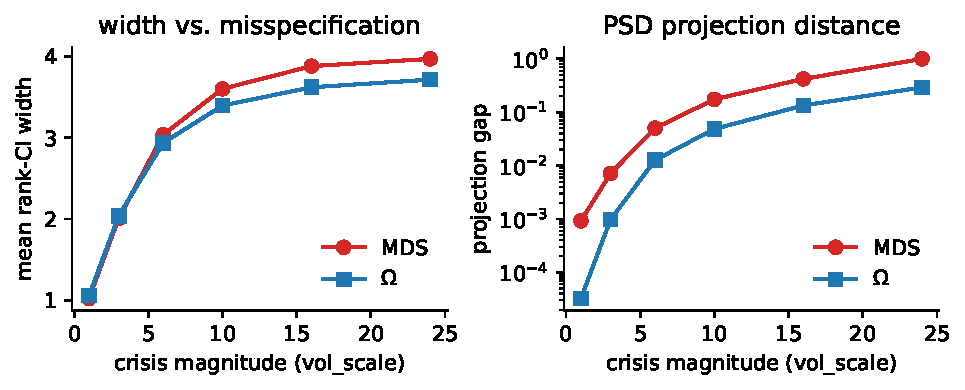
\includegraphics[width=\linewidth]{mc_crossover}
    \caption[Width crossover and projection distance]{Width crossover under growing
      non-stationarity, with imbalance fixed at $0.4$. \emph{Left:} the mean rank-CI
      width of the two constructions as the crisis magnitude grows; the direct
      construction ($\OmegaDirect$) becomes sharper than MDS. \emph{Right:} the MDS
      projection distance grows monotonically, driving the loss of calibration; the
      direct construction's distance, of a different matrix, is shown for reference. $R=500$,
      $B=2000$, $\alpha=0.05$.}
    \label{fig:mc-crossover}
  \end{figure}}

\newcommand{\figGjpCaterpillar}{%
  \begin{figure}[htb]
    \centering
    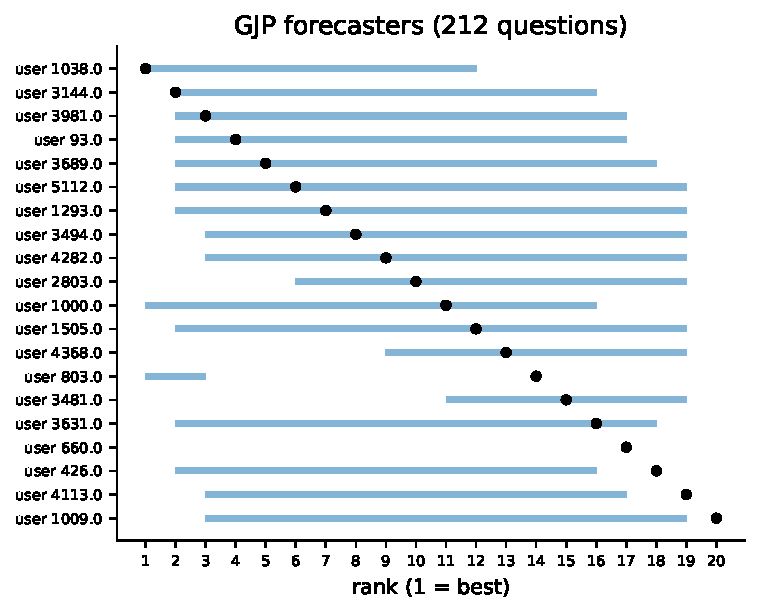
\includegraphics[width=0.72\linewidth]{gjp_caterpillar}
    \caption[GJP rank confidence sets]{Rank confidence sets for the twenty most active
      GJP forecasters (pooled tournament years~1--2, 212 questions, $\alpha=0.2$).
      Bars are the rank sets, dots the point ranks; forecasters are sorted best to
      worst. The best is confidently in the top three, the worst is pinned to last, and
      the middle remains wide --- the partial regime.}
    \label{fig:gjp-caterpillar}
  \end{figure}}

\newcommand{\figMcompCaterpillar}{%
  \begin{figure}[htb]
    \centering
    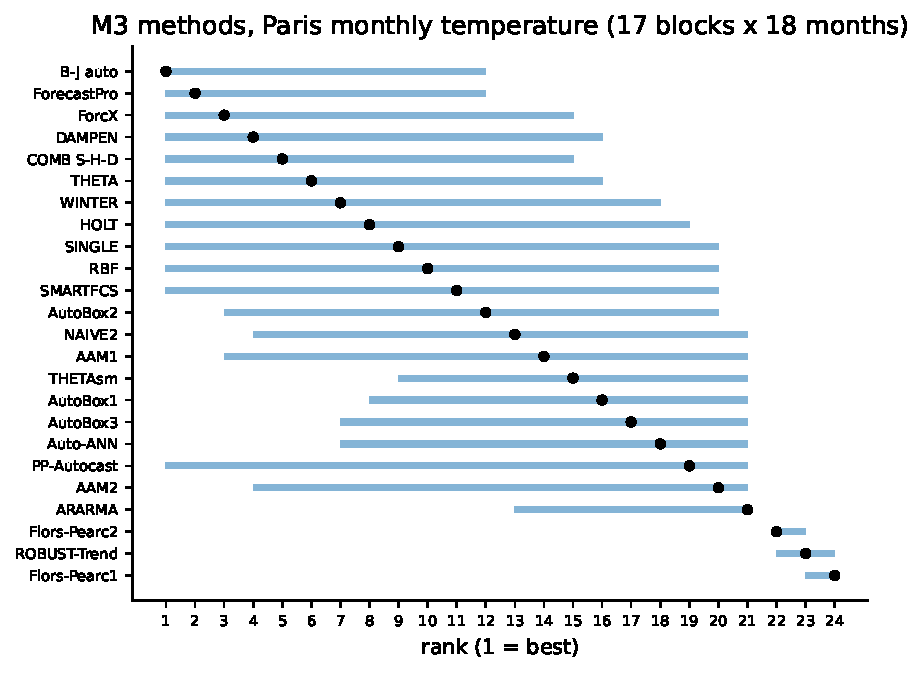
\includegraphics[width=0.75\linewidth]{mcomp_caterpillar}
    \caption[M3 methods on the Paris temperature record]{Rank confidence sets for the 24
      official M3 submissions on the Paris monthly temperature record (17 blocks
      $\times$ 18 held-out months, sMAPE, direct $\OmegaDirect$, $\alpha=0.1$). Bars are
      the rank sets, dots the point ranks. Twelve methods share rank one; three
      systematic failures are pinned to the last three ranks.}
    \label{fig:mcomp-caterpillar}
  \end{figure}}

\newcommand{\figSpfDepErrors}{%
  \begin{figure}[htb]
    \centering
    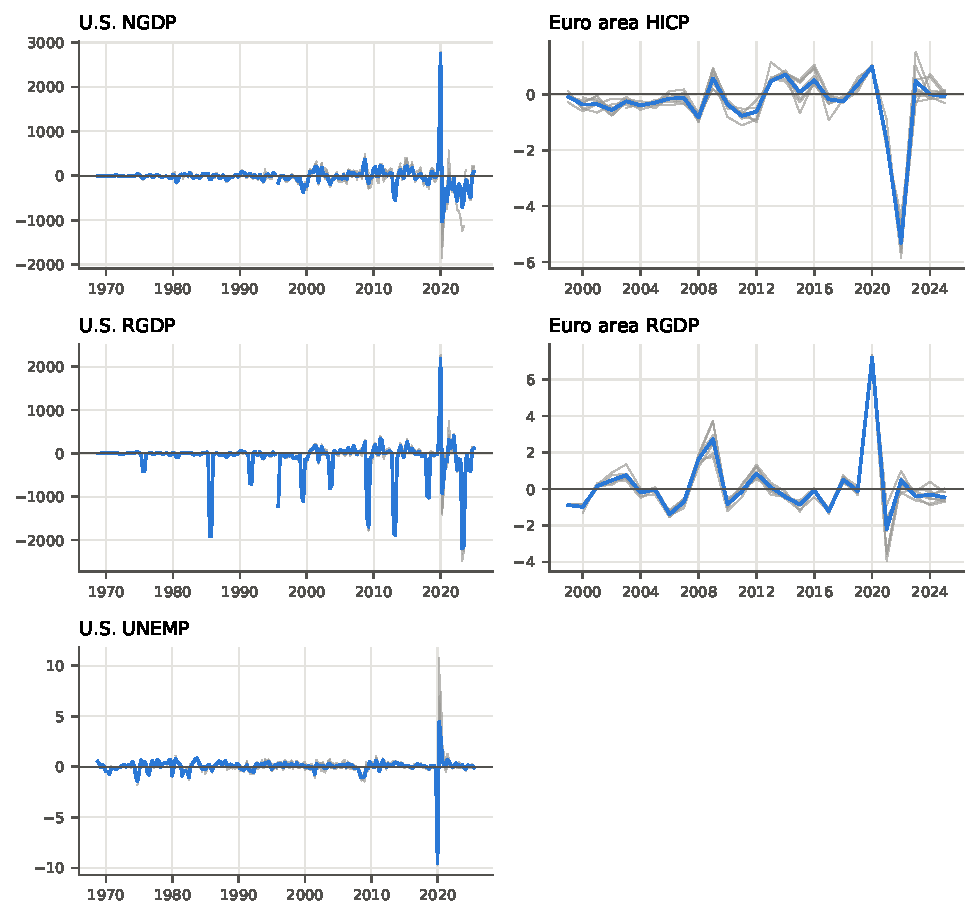
\includegraphics[width=0.9\linewidth]{spf_dep_errors}
    \caption[SPF forecast errors over time]{Forecast errors (forecast minus realization)
      of the eight best-covered forecasters (grey) and the cross-sectional mean of all
      forecasters (blue). Individual errors track the common component closely in every
      panel. The recurrent spikes in U.S.\ RGDP are base-year changes
      (Appendix~\ref{app:spf-dep-rebasing}).}
    \label{fig:spf-dep-errors}
  \end{figure}}

\newcommand{\figSpfDepAcf}{%
  \begin{figure}[htb]
    \centering
    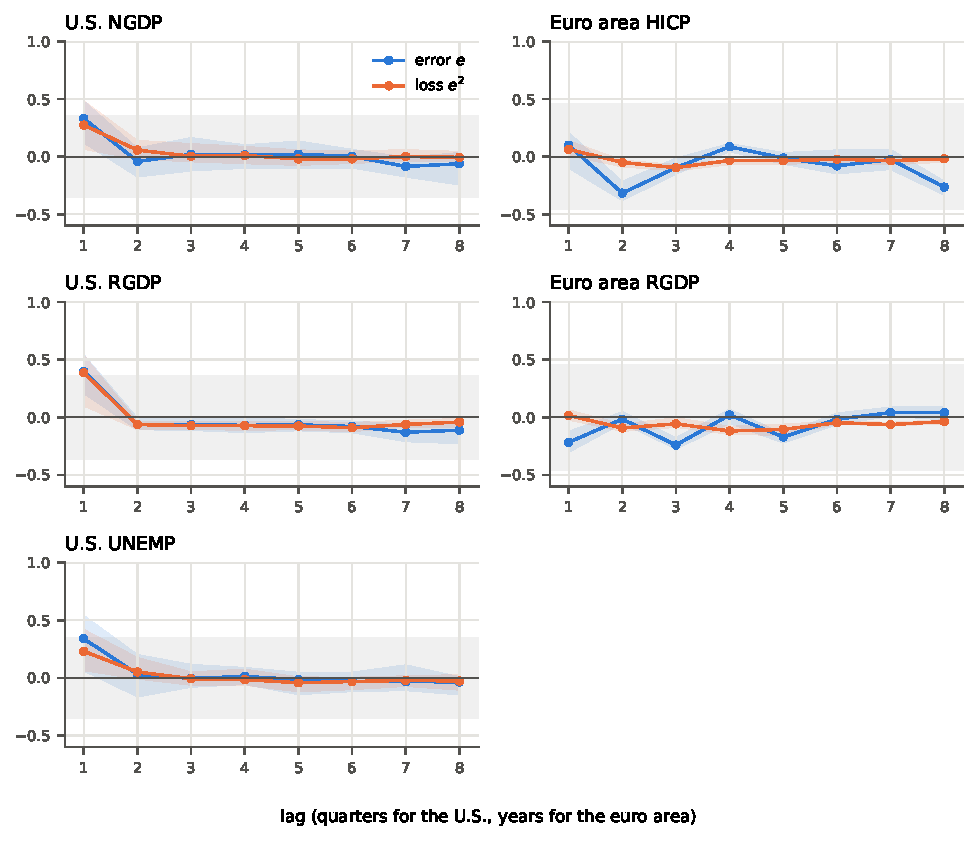
\includegraphics[width=0.9\linewidth]{spf_dep_acf}
    \caption[Autocorrelation of SPF errors and losses]{Autocorrelation of individual
      forecasters' errors $e$ and losses $e^2$: median across forecasters (line) and
      inter-quartile range (shaded). The grey band is the white-noise band
      $\pm1.96/\sqrt{n_1}$ at the median $n_1$.}
    \label{fig:spf-dep-acf}
  \end{figure}}
   % figure environments; chapters call \figMcCrossover, etc.
% ============================================================================
%  All table environments live in tables/. Chapters call \tabMcCoverage, etc.
%  (mirrors figures.tex; each command pulls in one file from tables/).
%  Result tables are written by scripts/make_thesis_tables.py and the notebooks in
%  the code repo (see Appendix A, Table tab:impl-repro); impl_* are hand-written.
% ============================================================================
\newcommand{\tabMcCoverage}{\begin{table}[htb]
  \centering
  \caption[Monte Carlo coverage and width]{Joint coverage, mean rank-CI width, and
  mean projection gap, MDS vs.\ direct-$\OmegaDirect$, with the joint circular block
  bootstrap (\textsc{cbb}, \S\ref{par:mbb}) as a covariance-free benchmark ($R=500$,
  $B=2000$, $\alpha=0.05$, identical panels). Coverage is at or above nominal for all three;
  on the balanced stationary designs they agree closely and the MDS gap is $\approx 0$;
  the MDS gap becomes non-zero and the width ordering flips only in the
  \emph{realistic} (non-stationary $+$ unbalanced) design,
  where the bootstrap sides with $\OmegaDirect$.}
  \label{tab:mc-coverage}
  \small
  \begin{tabular}{lcccccccc}
    \toprule
    & \multicolumn{3}{c}{joint coverage} & \multicolumn{3}{c}{mean width}
    & \multicolumn{2}{c}{projection gap}\\
    \cmidrule(lr){2-4}\cmidrule(lr){5-7}\cmidrule(lr){8-9}
    design & \textsc{mds} & $\OmegaDirect$ & \textsc{cbb} & \textsc{mds} & $\OmegaDirect$
    & \textsc{cbb} & \textsc{mds} & $\OmegaDirect$\\
    \midrule
    baseline & 1.000 & 1.000 & 1.000 & 0.450 & 0.453 & 0.450 & 0.000 & 0.000\\
    $\rho=0.6$ & 1.000 & 1.000 & 1.000 & 1.011 & 1.018 & 1.006 & 0.000 & 0.001\\
    $\rho=0.9$ & 0.968 & 0.968 & 0.966 & 1.996 & 2.023 & 1.958 & 0.000 & 0.004\\
    $\sigma_c=0$ & 1.000 & 1.000 & 1.000 & 0.444 & 0.446 & 0.445 & 0.000 & 0.000\\
    $\sigma_c=4$ & 1.000 & 1.000 & 1.000 & 0.458 & 0.466 & 0.467 & 0.000 & 0.000\\
    imbalance $0.4$ & 1.000 & 1.000 & 1.000 & 1.005 & 1.050 & 1.107 & 0.001 & 0.000\\
    non-stationary & 0.998 & 0.998 & 0.998 & 3.331 & 3.362 & 3.355 & 0.000 & 0.034\\
    \textbf{realistic} & 0.998 & 1.000 & 1.000 & \textbf{3.765} & \textbf{3.518} & 3.566 & 0.252 & 0.067\\
    \bottomrule
  \end{tabular}
\end{table}
}
\newcommand{\tabMcCrossover}{\begin{table}[htb]
  \centering
  \caption[Width crossover]{Width crossover under growing non-stationarity (imbalance
  fixed at $0.4$; larger \texttt{vol\_scale} $=$ bigger crisis episodes). As the MDS
  projection gap grows, its rank sets become wider than the direct construction's;
  bold marks the narrower route.}
  \label{tab:mc-crossover}
  \small
  \begin{tabular}{lcccccc}
    \toprule
    \texttt{vol\_scale} & 1 & 3 & 6 & 10 & 16 & 24\\
    \midrule
    \textsc{mds} width          & 1.02 & 2.01 & 3.04 & 3.60 & 3.88 & 3.97\\
    $\OmegaDirect$ width        & 1.06 & 2.04 & \textbf{2.94} & \textbf{3.39} & \textbf{3.62} & \textbf{3.71}\\
    \textsc{mds} projection gap & 0.00 & 0.01 & 0.05 & 0.17 & 0.42 & 1.00\\
    \bottomrule
  \end{tabular}
\end{table}
}
\newcommand{\tabSpfIndicators}{\begin{table}[htb]
  \centering
  \caption[SPF rank inference across indicators]{U.S.\ SPF rank inference across
  indicators (top-8 forecasters by coverage, one-quarter-ahead squared error, direct
  construction, $\alpha=0.2$, $B=5000$). No indicator names a best forecaster.
  ``Separated'' counts forecasters whose rank set is non-trivial; the last column is the
  rank set of the forecaster with the smallest mean loss.}
  \label{tab:spf-indicators}
  \small
  \begin{tabular}{lccccc}
    \toprule
    indicator & $p$ & quarters & $\max|t|$ & separated & best-forecaster CI\\
    \midrule
    NGDP (nominal output)      & 8 & 225 & 2.82 & 3 & $[1,8]$\\
    RGDP (real output)         & 8 & 225 & 2.80 & 2 & $[1,8]$\\
    UNEMP (unemployment rate)  & 8 & 228 & 4.04 & 7 & $[1,6]$\\
    \bottomrule
  \end{tabular}
\end{table}
}
\newcommand{\tabNgdp}{\begin{table}[htb]
  \centering
  \caption[NGDP rank confidence sets]{NGDP, top-5 SPF forecasters, one-quarter-ahead
  squared error ($\alpha=0.2$, $B=5000$). The MDS simulation loses calibration and
  reports the trivial $[1,5]$ throughout; the direct construction separates three
  forecasters.}
  \label{tab:ngdp}
  \small
  \begin{tabular}{lrcc}
    \toprule
    ID & mean MSE & CI (\textsc{mds}) & CI ($\OmegaDirect$)\\
    \midrule
    65  & 8{,}634   & $[1,5]$ & $[3,5]$\\
    84  & 9{,}874   & $[1,5]$ & $[1,5]$\\
    428 & 105{,}997 & $[1,5]$ & $[1,5]$\\
    426 & 122{,}073 & $[1,5]$ & $[1,4]$\\
    433 & 157{,}364 & $[1,5]$ & $[1,4]$\\
    \bottomrule
  \end{tabular}
\end{table}
}
\newcommand{\tabMcomp}{\begin{table}[htb]
  \centering
  \caption[M3 methods on the Paris temperature record]{Rank confidence sets for the 24
  official M3 submissions on the Paris monthly temperature record (17 blocks $\times$ 18
  held-out months, $n=306$), loss sMAPE, $\alpha=0.1$. Methods are sorted by mean sMAPE.
  Class: N = naive/simple, T = explicit trend (exponential smoothing), D = decomposition,
  A = ARIMA-type, E = expert system, NN = neural network. The twelve methods with a lower
  bound of $1$ form the $\tau$-best set for $\tau=1$.}
  \label{tab:mcomp}
  \small
  \begin{tabular}{llrcc}
    \toprule
    method & class & mean sMAPE & $\OmegaDirect$ & \MDS\\
    \midrule
    B-J automatic  & A  & 10.10 & $[1,12]$  & $[1,12]$\\
    ForecastPro    & E  & 10.13 & $[1,12]$  & $[1,12]$\\
    ForecastX      & E  & 10.39 & $[1,15]$  & $[1,15]$\\
    Dampen         & T  & 10.45 & $[1,16]$  & $[1,17]$\\
    Comb S-H-D     & T  & 10.46 & $[1,15]$  & $[1,15]$\\
    Theta          & D  & 10.50 & $[1,16]$  & $[1,16]$\\
    Winter         & T  & 10.66 & $[1,18]$  & $[1,18]$\\
    Holt           & T  & 10.86 & $[1,19]$  & $[1,19]$\\
    Single         & N  & 10.92 & $[1,20]$  & $[1,21]$\\
    RBF            & E  & 10.95 & $[1,20]$  & $[1,20]$\\
    SmartFcs       & E  & 11.02 & $[1,20]$  & $[1,20]$\\
    AutoBox2       & A  & 11.26 & $[3,20]$  & $[3,20]$\\
    Naive2         & N  & 11.62 & $[4,21]$  & $[4,21]$\\
    AAM1           & A  & 11.96 & $[3,21]$  & $[3,21]$\\
    Theta-sm       & T  & 12.23 & $[9,21]$  & $[9,21]$\\
    AutoBox1       & A  & 12.45 & $[8,21]$  & $[8,21]$\\
    AutoBox3       & A  & 12.53 & $[7,21]$  & $[6,21]$\\
    Automat ANN    & NN & 12.57 & $[7,21]$  & $[7,21]$\\
    PP-Autocast    & T  & 12.79 & $[1,21]$  & $[1,21]$\\
    AAM2           & A  & 12.91 & $[4,21]$  & $[4,21]$\\
    ARARMA         & A  & 14.09 & $[13,21]$ & $[12,21]$\\
    Flores-Pearce2 & E  & 26.89 & $[22,23]$ & $[22,23]$\\
    Robust-Trend   & T  & 27.77 & $[22,24]$ & $[22,24]$\\
    Flores-Pearce1 & E  & 37.80 & $[23,24]$ & $[23,24]$\\
    \bottomrule
  \end{tabular}
\end{table}
}
\newcommand{\tabThreeRegimes}{\begin{table}[htb]
  \centering
  \caption[The three regimes]{The three applications under the same procedure (direct
  construction, $\alpha=0.1$ for all three; the SPF and GJP sections use $\alpha=0.2$).
  Normalized width is the mean rank-CI width divided by $p-1$; ``separated'' is the
  fraction of units with a non-trivial set; ``exact'' counts units pinned to a single
  rank.}
  \label{tab:threeregimes}
  \small
  \begin{tabular}{lccccl}
    \toprule
    dataset & $p$ & obs & norm.\ width & separated & exact ranks\\
    \midrule
    macro (NGDP)           & 8 & 225 & 0.96 & 25\% & 0 \ (\emph{null})\\
    GJP (geopolitical)     & 20 & 212 & 0.73 & 100\% & 1 \ (\emph{partial})\\
    M3 (Paris temperature) & 24 & 306 & 0.59 & 100\% & 0 \ (\emph{informative})\\
    \bottomrule
  \end{tabular}
\end{table}
}
\newcommand{\tabSpfDepPanels}{\begin{table}[htb]
  \centering
  \caption[SPF error panels]{Error panels used in the dependence analysis. ``Forecasters'' counts those with at
  least 20 (U.S.) or 15 (euro area) observations; coverage is the share of non-missing cells among the eight
  best-covered forecasters, the panel the rank inference uses.}
  \label{tab:spf-dep-panels}
  \small
  \begin{tabular}{llrrr}
    \toprule
    panel & sample & periods & forecasters & top-8 coverage\\
    \midrule
    U.S.\ NGDP & 1968Q4 -- 2025Q1 & 226 & 148 & 52\%\\
    U.S.\ RGDP & 1968Q4 -- 2025Q1 & 226 & 147 & 52\%\\
    U.S.\ UNEMP & 1968Q4 -- 2025Q3 & 228 & 151 & 52\%\\
    Euro area HICP & 1999 -- 2025 & 27 & 58 & 99\%\\
    Euro area RGDP & 1999 -- 2025 & 27 & 58 & 99\%\\
    \midrule
    U.S.\ NGDP, growth$^\dagger$ & 1968Q4 -- 2025Q1 & 226 & 148 & 52\%\\
    U.S.\ RGDP, growth$^\dagger$ & 1968Q4 -- 2025Q1 & 226 & 147 & 52\%\\
    \bottomrule
  \end{tabular}
\end{table}
}
\newcommand{\tabSpfDepSerial}{\begin{table}[htb]
  \centering
  \caption[Serial dependence in SPF errors]{Serial dependence. Columns 2--5 are per-forecaster statistics over all
  forecasters in Table~\ref{tab:spf-dep-panels}: the median lag-1 autocorrelation of the signed error $e$ and of the
  loss $e^2$, the share of forecasters whose lag-1 autocorrelation lies outside the $\pm1.96/\sqrt{n_1}$ band, and the
  share rejecting the Box--Pierce test (4 lags U.S., 2 lags euro area) at 5\%. Columns 6--7 refer to the 28 pairwise
  loss differences $d^{jk}$ of the top-8 forecasters: the median AR(1) coefficient and the median Andrews bandwidth.
  Under no serial correlation about 5\% of forecasters would be flagged. $^\dagger$Robustness: the same forecasts
  as annualized quarter-on-quarter growth rates.}
  \label{tab:spf-dep-serial}
  \small
  \begin{tabular}{lcccccc}
    \toprule
    & \multicolumn{4}{c}{individual errors} & \multicolumn{2}{c}{loss differences}\\
    \cmidrule(lr){2-5}\cmidrule(lr){6-7}
    panel & $\hat\rho_1(e)$ & $\hat\rho_1(e^2)$ & lag-1 sig. & BP rej. & AR(1) of $d^{jk}$ & $\hat L$\\
    \midrule
    U.S.\ NGDP & 0.33 & 0.27 & 43\% & 34\% & 0.11 & 3\\
    U.S.\ RGDP & 0.40 & 0.39 & 63\% & 44\% & 0.00 & 1\\
    U.S.\ UNEMP & 0.34 & 0.23 & 55\% & 34\% & 0.01 & 2\\
    Euro area HICP & 0.10 & 0.06 & 3\% & 0\% & $-0.13$ & 1\\
    Euro area RGDP & $-0.22$ & 0.02 & 2\% & 0\% & $-0.06$ & 1\\
    \midrule
    U.S.\ NGDP, growth$^\dagger$ & 0.10 & 0.14 & 29\% & 15\% & 0.07 & 1\\
    U.S.\ RGDP, growth$^\dagger$ & 0.09 & 0.16 & 29\% & 11\% & $-0.03$ & 1\\
    \bottomrule
  \end{tabular}
\end{table}
}
\newcommand{\tabSpfDepCross}{\begin{table}[htb]
  \centering
  \caption[Cross-sectional dependence in SPF errors]{Cross-sectional dependence of the errors. Mean pairwise
  correlation of signed errors (Pearson and Spearman) and of losses $e^2$, over all forecaster pairs in
  Table~\ref{tab:spf-dep-panels} with at least eight common periods; Pesaran's CD statistic for the signed errors
  ($\approx\Normal(0,1)$ under cross-sectional independence); and the share of the pooled error variance explained
  by a common period effect, with its value under no common component in parentheses. $^\dagger$As in
  Table~\ref{tab:spf-dep-serial}.}
  \label{tab:spf-dep-cross}
  \small
  \begin{tabular}{lccccc}
    \toprule
    panel & $\bar\rho(e)$ & $\bar\rho_S(e)$ & $\bar\rho(e^2)$ & CD & period $R^2$\\
    \midrule
    U.S.\ NGDP & 0.77 & 0.71 & 0.69 & 255 & 0.89 (0.03)\\
    U.S.\ RGDP & 0.92 & 0.80 & 0.89 & 301 & 0.98 (0.03)\\
    U.S.\ UNEMP & 0.76 & 0.67 & 0.65 & 250 & 0.82 (0.03)\\
    Euro area HICP & 0.89 & 0.79 & 0.82 & 147 & 0.93 (0.02)\\
    Euro area RGDP & 0.97 & 0.91 & 0.97 & 160 & 0.96 (0.02)\\
    \midrule
    U.S.\ NGDP, growth$^\dagger$ & 0.74 & 0.69 & 0.64 & 242 & 0.82 (0.03)\\
    U.S.\ RGDP, growth$^\dagger$ & 0.77 & 0.71 & 0.68 & 254 & 0.81 (0.03)\\
    \bottomrule
  \end{tabular}
\end{table}
}
\newcommand{\tabSpfDepDiff}{\begin{table}[htb]
  \centering
  \caption[The common shock in loss differences]{The common shock in the loss differences of the top-8
  forecasters. ``Cancelled'' is the median over pairs of $2\Cov(X_j,X_k)/(\Var X_j+\Var X_k)$, the share of the
  loss variance removed by differencing. The remaining columns relate the cross-pair mean of $(d^{jk}_t)^2$ to the
  squared consensus error $\bar e_t^{\,2}$: their Spearman correlation, and the share of $\sum_t (d^{jk}_t)^2$ that
  falls in the 10\% of periods with the largest $\bar e_t^{\,2}$, on the full sample and without 2020--21.
  $^\dagger$As in Table~\ref{tab:spf-dep-serial}.}
  \label{tab:spf-dep-diff}
  \small
  \begin{tabular}{lccccc}
    \toprule
    & & \multicolumn{2}{c}{$\rho_S\big(\bar e_t^{\,2},\,\overline{d_t^{\,2}}\big)$}
      & \multicolumn{2}{c}{share in top-10\% periods}\\
    \cmidrule(lr){3-4}\cmidrule(lr){5-6}
    panel & cancelled & full & ex-2020/21 & full & ex-2020/21\\
    \midrule
    U.S.\ NGDP & 0.91 & 0.76 & 0.74 & 96\% & 92\%\\
    U.S.\ RGDP & 1.00 & 0.87 & 0.86 & 96\% & 99\%\\
    U.S.\ UNEMP & 0.82 & 0.71 & 0.61 & 100\% & 73\%\\
    Euro area HICP & 0.97 & 0.63 & 0.65 & 94\% & 94\%\\
    Euro area RGDP & 0.98 & 0.89 & 0.87 & 96\% & 92\%\\
    \midrule
    U.S.\ NGDP, growth$^\dagger$ & 0.75 & 0.68 & 0.67 & 84\% & 31\%\\
    U.S.\ RGDP, growth$^\dagger$ & 0.81 & 0.73 & 0.72 & 99\% & 71\%\\
    \bottomrule
  \end{tabular}
\end{table}
}
\newcommand{\tabImplCode}{\begin{table}[htb]
  \centering
  \caption[From the method to the code]{Where each step of the procedure is
  implemented. Paths are relative to \texttt{src/rankci/}; equation and section
  numbers refer to the main text.}
  \label{tab:impl-code}
  \small
  \begin{tabular}{p{5.4cm}p{8.4cm}}
    \toprule
    step & module: function\\
    \midrule
    Contrasts $\Deltahat_{j,k}$ and HAC standard errors $\seNW{jk}$,
    \eqref{eq:contrast}, \eqref{eq:nw}, \eqref{eq:senw}
      & \texttt{core/pairwise.py}: \texttt{compute\_pairwise}, \texttt{nw\_se}\\
    Andrews plug-in bandwidth \eqref{eq:andrews}
      & \texttt{core/bandwidth.py}: \texttt{andrews\_bandwidth},
        \texttt{andrews\_alpha1}, \texttt{ar1\_coefficient}\\
    MDS covariance \eqref{eq:doublecentre} and its projection
    (\S\ref{sec:mds-psd})
      & \texttt{core/pairwise.py}: \texttt{cov\_theta\_pairwise}\\
    Direct covariance \eqref{eq:omega-entry} and its projection
    (\S\ref{sec:omega-psd})
      & \texttt{core/omega.py}: \texttt{cov\_via\_omega}\\
    Stacked balanced estimator \eqref{eq:omega-balanced}
      & \texttt{core/omega.py}: \texttt{stacked\_nw\_balanced} (reference for the
        tests only)\\
    Studentized null draws, the seam (\S\ref{sec:seam})
      & \texttt{core/covariance.py}: \texttt{studentized\_null\_draws}\\
    Romano--Wolf stepdown (\S\ref{sec:stepdown}) and rank sets
    \eqref{eq:rankset}
      & \texttt{core/covariance.py}: \texttt{stepdown\_rank\_ci};\newline
        \texttt{core/pairwise.py}: \texttt{rank\_ci\_from\_rejections}\\
    Complete procedure
      & \texttt{core/stepwise\_simulation.py}:\newline
        \texttt{rank\_ci\_stepwise\_simulation\_pairwise}\\
    Marginal rank sets
      & \texttt{core/stepwise.py}: \texttt{rank\_ci\_marginal\_pairwise} (block bootstrap)\\
    $\tau$-best sets (\S\ref{sec:taubest})
      & \texttt{core/tau\_best.py}: \texttt{tau\_best\_from\_rank\_ci}
        (projection), \texttt{tau\_best\_simulation\_pairwise} (MDS)\\
    Block bootstrap benchmark (\S\ref{par:mbb})
      & \texttt{core/block\_bootstrap.py}: \texttt{mbb\_indices},
        \texttt{default\_block\_length}, \texttt{block\_bootstrap\_draws};
        \texttt{core/stepwise.py}: \texttt{rank\_ci\_stepwise\_pairwise}\\
    Monte Carlo design \eqref{eq:dgp} and coverage study
      & \texttt{sim.py}: \texttt{simulate\_panel}, \texttt{coverage\_study}\\
    Loss panels of the applications
      & \texttt{data/philly.py}, \texttt{data/ecb.py}, \texttt{data/gjp.py};
        \texttt{data/mcomp.py}: \texttt{official\_panel};
        \texttt{data/panel.py}: \texttt{select\_top\_forecasters}\\
    \bottomrule
  \end{tabular}
\end{table}
}
\newcommand{\tabImplEnv}{\begin{table}[htb]
  \centering
  \caption[Software environment]{Software used for the reported results (Python
  3.11.5, macOS 14.6, Apple silicon). The \texttt{rankci} package itself requires
  only NumPy and pandas.}
  \label{tab:impl-env}
  \small
  \begin{tabular}{llp{7.6cm}}
    \toprule
    package & version & used for\\
    \midrule
    NumPy      & 2.4.6  & arrays, linear algebra, random numbers\\
    pandas     & 2.3.3  & data loading and panel construction\\
    openpyxl   & 3.1.5  & reading the Philadelphia Fed and Eurostat Excel files\\
    rdata      & 1.1.0  & reading the R data files of the M3 forecasts\\
    SciPy      & 1.17.1 & tests and rank correlations in
                          Appendix~\ref{app:spf-dependence}\\
    Matplotlib & 3.11.1 & figures\\
    ipykernel, nbconvert & 7.3.0, 7.17.1 & executing the notebooks\\
    pytest     & 9.1.1  & unit tests\\
    \bottomrule
  \end{tabular}
\end{table}
}
\newcommand{\tabImplTests}{\begin{table}[htb]
  \centering
  \caption[Unit tests]{The unit tests in \texttt{tests/} (65 in total). All pass; one
  downloads data and runs only on request.}
  \label{tab:impl-tests}
  \small
  \begin{tabular}{lcp{9.6cm}}
    \toprule
    file & tests & what is checked\\
    \midrule
    \texttt{test\_bandwidth.py} & 6
      & $\hat\alpha(1)$ and $L$ match the closed forms \eqref{eq:alpha1} and
        \eqref{eq:andrews}; white noise gives a small bandwidth; the bandwidth
        grows with persistence; $\hat\rho$ is clamped; short series get $L=0$.\\
    \texttt{test\_omega.py} & 11
      & $\Omegahat_{aa}=(\seNW{a})^2$ on a balanced panel; on an unbalanced panel
        the diagonal matches an independently coded long-run variance; with a
        common bandwidth $\Omegahat$ equals the stacked estimator
        \eqref{eq:omega-balanced} entrywise (nesting); the seam studentizes by
        $\sqrt{\Omegahat^{+}_{aa}}$; balanced with a common bandwidth is PSD
        without projection, while the per-series bandwidth may need it
        (\S\ref{sec:caveat}); the projected matrix is PSD; cross-products use
        only jointly observed rows; off-diagonal entries are divided by $n_a n_b$;
        on an unbalanced panel with a common bandwidth the unprojected matrix is
        PSD \eqref{eq:omega-congruence}; and, by simulation, its off-diagonal entries
        track the sampling covariance of the difference means.\\
    \texttt{test\_seam.py} & 5
      & draw shapes for both constructions; trivial sets $[1,p]$ on i.i.d.\
        panels with equal means; the two constructions agree on a balanced,
        well-separated panel; rank sets are well formed; a smaller $\alpha$
        gives wider sets.\\
    \texttt{test\_sim.py} & 8
      & panel shape and means; the common shock cancels in differences; AR(1)
        stationary variance; staggered entry and exit; true ranks; volatility
        episodes raise local variance; coverage-study output; joint coverage near
        nominal on an easy balanced design.\\
    \texttt{test\_block\_bootstrap.py} & 12
      & block indices are contiguous runs within $[0,n)$, wrapping around when
        circular; circular blocks draw every row equally often, non-circular ones
        under-sample the first and last rows; $\ell=1$ is the i.i.d.\ row bootstrap;
        $\ell=L+1$ and the cap at $n$; the block length grows with persistence; with
        $\ell=L+1$ the bootstrap variance of a mean equals the Newey--West variance;
        pairwise means skip rows without overlap; the stepdown draws once, with
        non-increasing critical values, and equals the shared stepdown applied to one
        array of draws; the engines run on an unbalanced panel and are
        seed-reproducible.\\
    \texttt{test\_tau\_best.py} & 3
      & the $\tau$-best projection of \S\ref{sec:taubest} keeps a unit with
        $U_j<\tau$ (rank set $[1,1]$ at $\tau=2$); for $\tau=1$ it is the set of units
        whose rank set contains rank one; when every rank set covers the true rank, each
        $\tau$-best set contains all truly top-$\tau$ units.\\
    \texttt{test\_gjp.py} & 7
      & daily-averaged Brier score on hand-computed cases (single binary
        forecast, carry-forward, multi-category, withdrawals, outcome never
        assigned); panel shape, row order and filters.\\
    \texttt{test\_mcomp.py} & 13
      & the Paris panel of the official M3 forecasts, built from a stored copy of
        its 306 rows: shape, calendar order, the mean sMAPEs of
        Table~\ref{tab:mcomp}, methods with missing forecasts dropped; with
        \texttt{RANKCI\_NETWORK=1}, the download from CRAN reproduces that copy;
        sMAPE and MASE, and re-implemented forecasting methods that are not used
        for any reported result.\\
    \bottomrule
  \end{tabular}
\end{table}
}
\newcommand{\tabImplRepro}{\begin{table}[htb]
  \centering
  \caption[Which file produces each result]{Which file produces each result.
  Notebooks are in \texttt{notebooks/}, scripts in \texttt{scripts/}. Every reported
  rank set comes from the simulation route of \S\ref{sec:studentized}; the block
  bootstrap of \S\ref{par:mbb} appears only as a benchmark. All runs use seed $42$
  unless stated otherwise.}
  \label{tab:impl-repro}
  \small
  \begin{tabular}{p{4.2cm}p{4.6cm}p{5.0cm}}
    \toprule
    result & file & settings\\
    \midrule
    Tables~\ref{tab:mc-coverage} and~\ref{tab:mc-crossover}; tie design
    (\S\ref{sec:mc-coverage})
      & \texttt{make\_thesis\_tables.py}, in the same run as
        Tables~\ref{tab:app-mc-coverage}--\ref{tab:app-mc-crossover}
        (designs of \texttt{01\_toydataset})
      & $R=500$, $B=2000$, $\alpha=0.05$; seeds as in \S\ref{app:impl-details}\\
    Figure~\ref{fig:mc-crossover}
      & \texttt{make\_thesis\_figures.py}
      & the crossover designs and seeds of Table~\ref{tab:mc-crossover}\\
    NGDP draw diagnostics (\S\ref{sec:mc-mechanism})
      & \texttt{01\_toydataset}, last section
      & top-5 NGDP panel, $B=20000$, seed $1$, $\alpha=0.05$\\
    Tables~\ref{tab:spf-dep-panels}--\ref{tab:spf-dep-diff},
    Figures~\ref{fig:spf-dep-errors} and~\ref{fig:spf-dep-acf}
      & \texttt{02\_primary\_analysis}
      & deterministic\\
    Table~\ref{tab:spf-indicators}
      & \texttt{make\_thesis\_tables.py}
      & direct construction, top-8, $\alpha=0.2$, $B=5000$; MDS in the text\\
    Table~\ref{tab:ngdp}; $\tau$-best sets for NGDP (\S\ref{sec:apps-spf})
      & \texttt{make\_thesis\_tables.py}
      & top-5, $\alpha=0.2$, $B=5000$, MDS and direct; $\tau$-best sets projected
        from the direct rank sets\\
    Euro-area results (\S\ref{sec:apps-ecb})
      & \texttt{make\_thesis\_tables.py}
      & top-8 with at least $15$ observations, $\alpha=0.2$, $B=5000$, MDS and direct\\
    GJP results (\S\ref{sec:apps-gjp})
      & \texttt{gjp/GJP\_CI}
      & top-20 individuals with at least $60$ questions, years 1--2,
        $\alpha=0.2$, $B=5000$, direct construction; $\tau$-best set projected from
        its rank sets; split-half check\\
    Figure~\ref{fig:gjp-caterpillar}
      & \texttt{make\_thesis\_figures.py}
      & as for the GJP results, direct construction\\
    Table~\ref{tab:mcomp} and every number in \S\ref{sec:apps-mcomp} except the
    block-bootstrap comparison
      & \texttt{mcomp/MCOMP\_CI}
      & $\alpha=0.1$, $B=20000$, direct and MDS; robustness at $\alpha=0.05$ and on
        block averages\\
    Figure~\ref{fig:mcomp-caterpillar}
      & \texttt{make\_thesis\_figures.py}
      & direct construction, $\alpha=0.1$, $B=20000$\\
    Table~\ref{tab:threeregimes}
      & \texttt{make\_thesis\_tables.py}
      & direct construction, $\alpha=0.1$, $B=20000$; NGDP top-8\\
    Tables~\ref{tab:app-mc-coverage}--\ref{tab:app-mc-crossover}
      & \texttt{make\_thesis\_tables.py}
      & the designs and seeds of \texttt{01\_toydataset}; MDS, direct and block
        bootstrap; skipped with \texttt{--skip-mc}\\
    Tables~\ref{tab:app-spf-sets}--\ref{tab:app-gjp}
      & \texttt{make\_thesis\_tables.py}
      & as for Table~\ref{tab:spf-indicators}, \S\ref{sec:apps-ecb} and the GJP
        results; MDS and direct\\
    Tables~\ref{tab:app-m3-blocks} and~\ref{tab:app-m3-robust}
      & \texttt{make\_thesis\_tables.py}
      & direct construction, $\alpha=0.1$ (and $0.05$), $B=20000$\\
    Block-bootstrap comparisons in Chapter~\ref{ch:apps}
      & \texttt{make\_thesis\_tables.py} (printed)
      & block bootstrap with $B=5000$ against the direct construction at the level
        of each result: $\alpha=0.2$, M3 $\alpha=0.1$\\
    \bottomrule
  \end{tabular}
\end{table}
}
% Appendix B (app:additional), all written by scripts/make_thesis_tables.py
\newcommand{\tabAppMcCoverage}{\begin{table}[htb]
  \centering
  \caption[Monte Carlo coverage, full grid]{Joint coverage and the smallest marginal coverage over the five forecasters, for every design of the Monte Carlo grid ($R=500$, $B=2000$, nominal level $0.95$; identical panels for the three routes). The last row is the rate at which a tied pair of the tie design is confidently ordered, averaged over the two tied pairs and the replications.}
  \label{tab:app-mc-coverage}
  \small
  \begin{tabular}{lcccccc}
    \toprule
    & \multicolumn{3}{c}{joint coverage} & \multicolumn{3}{c}{min.\ marginal coverage}\\
    \cmidrule(lr){2-4}\cmidrule(lr){5-7}
    design & \textsc{mds} & $\OmegaDirect$ & \textsc{cbb} & \textsc{mds} & $\OmegaDirect$ & \textsc{cbb}\\
    \midrule
    baseline & 1.000 & 1.000 & 1.000 & 1.000 & 1.000 & 1.000\\
    $\rho=0$ & 1.000 & 1.000 & 1.000 & 1.000 & 1.000 & 1.000\\
    $\rho=0.6$ & 1.000 & 1.000 & 1.000 & 1.000 & 1.000 & 1.000\\
    $\rho=0.9$ & 0.968 & 0.968 & 0.966 & 0.984 & 0.984 & 0.982\\
    $\sigma_c=0$ & 1.000 & 1.000 & 1.000 & 1.000 & 1.000 & 1.000\\
    $\sigma_c=4$ & 1.000 & 1.000 & 1.000 & 1.000 & 1.000 & 1.000\\
    imbalance $0.2$ & 1.000 & 1.000 & 1.000 & 1.000 & 1.000 & 1.000\\
    imbalance $0.4$ & 1.000 & 1.000 & 1.000 & 1.000 & 1.000 & 1.000\\
    non-stationary & 0.998 & 0.998 & 0.998 & 0.998 & 0.998 & 0.998\\
    realistic & 0.998 & 1.000 & 1.000 & 0.998 & 1.000 & 1.000\\
    \midrule
    ties: false separation & 0.020 & 0.019 & 0.020 & & & \\
    \bottomrule
  \end{tabular}
\end{table}
}
\newcommand{\tabAppMcWidth}{\begin{table}[htb]
  \centering
  \caption[Monte Carlo width and projection distance, full grid]{Mean rank-set width, mean projection distance $\Frob{A-A^{+}}$ of the matrix each simulation route draws from, and mean number of stepdown rounds, for every design of the Monte Carlo grid ($R=500$, $B=2000$, $\alpha=0.05$).}
  \label{tab:app-mc-width}
  \small
  \begin{tabular}{lccccccc}
    \toprule
    & \multicolumn{3}{c}{mean width} & \multicolumn{2}{c}{projection distance} & \multicolumn{2}{c}{stepdown rounds}\\
    \cmidrule(lr){2-4}\cmidrule(lr){5-6}\cmidrule(lr){7-8}
    design & \textsc{mds} & $\OmegaDirect$ & \textsc{cbb} & \textsc{mds} & $\OmegaDirect$ & \textsc{mds} & $\OmegaDirect$\\
    \midrule
    baseline & 0.450 & 0.453 & 0.450 & 0.000 & 0.000 & 2.21 & 2.22\\
    $\rho=0$ & 0.114 & 0.110 & 0.110 & 0.000 & 0.001 & 2.11 & 2.13\\
    $\rho=0.6$ & 1.011 & 1.018 & 1.006 & 0.000 & 0.001 & 2.18 & 2.18\\
    $\rho=0.9$ & 1.996 & 2.023 & 1.958 & 0.000 & 0.004 & 2.13 & 2.14\\
    $\sigma_c=0$ & 0.444 & 0.446 & 0.445 & 0.000 & 0.000 & 2.20 & 2.20\\
    $\sigma_c=4$ & 0.458 & 0.466 & 0.467 & 0.000 & 0.000 & 2.20 & 2.21\\
    imbalance $0.2$ & 0.662 & 0.678 & 0.682 & 0.000 & 0.000 & 2.21 & 2.22\\
    imbalance $0.4$ & 1.005 & 1.050 & 1.107 & 0.001 & 0.000 & 2.20 & 2.23\\
    non-stationary & 3.331 & 3.362 & 3.355 & 0.000 & 0.034 & 1.79 & 1.76\\
    realistic & 3.765 & 3.518 & 3.566 & 0.252 & 0.067 & 1.41 & 1.55\\
    ties & 0.786 & 0.787 & 0.786 & 0.000 & 0.000 & 2.02 & 2.01\\
    \bottomrule
  \end{tabular}
\end{table}
}
\newcommand{\tabAppMcCrossover}{\begin{table}[htb]
  \centering
  \caption[Crossover sweep, full results]{The crossover sweep of Table~\ref{tab:mc-crossover} with the coverage and the projection distance of both routes (imbalance $0.4$, five volatility episodes of growing scale, $R=500$, $B=2000$, $\alpha=0.05$).}
  \label{tab:app-mc-crossover}
  \small
  \begin{tabular}{ccccccc}
    \toprule
    & \multicolumn{2}{c}{joint coverage} & \multicolumn{2}{c}{mean width} & \multicolumn{2}{c}{projection distance}\\
    \cmidrule(lr){2-3}\cmidrule(lr){4-5}\cmidrule(lr){6-7}
    \texttt{vol\_scale} & \textsc{mds} & $\OmegaDirect$ & \textsc{mds} & $\OmegaDirect$ & \textsc{mds} & $\OmegaDirect$\\
    \midrule
    1 & 1.000 & 1.000 & 1.023 & 1.060 & 0.001 & 0.000\\
    3 & 1.000 & 1.000 & 2.009 & 2.039 & 0.007 & 0.001\\
    6 & 1.000 & 1.000 & 3.035 & 2.936 & 0.050 & 0.013\\
    10 & 1.000 & 1.000 & 3.600 & 3.394 & 0.174 & 0.049\\
    16 & 1.000 & 1.000 & 3.879 & 3.619 & 0.420 & 0.134\\
    24 & 1.000 & 1.000 & 3.968 & 3.713 & 0.996 & 0.291\\
    \bottomrule
  \end{tabular}
\end{table}
}
\newcommand{\tabAppSpfSets}{\begin{table}[htb]
  \centering
  \caption[U.S. SPF: all rank sets]{Rank confidence sets of the eight best-covered U.S.\ SPF forecasters, the full sets behind Table~\ref{tab:spf-indicators} (one-quarter-ahead squared error, $\alpha=0.2$, $B=5000$). Forecasters are sorted by mean loss; ``obs.''\ is the number of quarters in which a forecaster reported. The loss is in squared billions of dollars for NGDP and RGDP and in squared percentage points for UNEMP.}
  \label{tab:app-spf-sets}
  \small
  \begin{tabular}{rrrcc}
    \toprule
    ID & obs. & mean loss & $\OmegaDirect$ & \textsc{mds}\\
    \midrule
    \multicolumn{5}{l}{\emph{nominal output (NGDP), 225 quarters}}\\
    40 & 107 & 7{,}484 & $[1,8]$ & $[1,8]$\\
    65 & 122 & 8{,}634 & $[3,8]$ & $[1,8]$\\
    84 & 119 & 9{,}874 & $[1,8]$ & $[1,8]$\\
    428 & 117 & 105{,}997 & $[1,8]$ & $[1,8]$\\
    421 & 114 & 106{,}525 & $[1,8]$ & $[1,8]$\\
    426 & 121 & 122{,}073 & $[1,7]$ & $[1,8]$\\
    411 & 115 & 133{,}745 & $[1,8]$ & $[1,8]$\\
    433 & 119 & 157{,}364 & $[1,7]$ & $[1,8]$\\
    \addlinespace
    \multicolumn{5}{l}{\emph{real output (RGDP), 225 quarters}}\\
    65 & 124 & 111{,}180 & $[1,8]$ & $[1,8]$\\
    40 & 104 & 125{,}550 & $[1,8]$ & $[1,8]$\\
    84 & 117 & 142{,}812 & $[1,7]$ & $[1,8]$\\
    421 & 120 & 242{,}178 & $[1,8]$ & $[1,8]$\\
    433 & 120 & 303{,}832 & $[1,8]$ & $[1,8]$\\
    428 & 117 & 312{,}332 & $[1,8]$ & $[1,8]$\\
    411 & 115 & 316{,}620 & $[1,8]$ & $[1,8]$\\
    426 & 121 & 320{,}346 & $[2,8]$ & $[1,8]$\\
    \addlinespace
    \multicolumn{5}{l}{\emph{unemployment rate (UNEMP), 228 quarters}}\\
    84 & 122 & 0.149 & $[1,6]$ & $[1,8]$\\
    65 & 124 & 0.205 & $[6,8]$ & $[1,8]$\\
    428 & 120 & 0.868 & $[1,7]$ & $[1,8]$\\
    463 & 106 & 0.947 & $[1,8]$ & $[1,8]$\\
    433 & 123 & 1.048 & $[1,7]$ & $[1,8]$\\
    421 & 122 & 1.331 & $[2,8]$ & $[1,8]$\\
    426 & 122 & 1.384 & $[1,7]$ & $[1,8]$\\
    411 & 118 & 1.880 & $[1,7]$ & $[1,8]$\\
    \bottomrule
  \end{tabular}
\end{table}
}
\newcommand{\tabAppEcbSets}{\begin{table}[htb]
  \centering
  \caption[Euro-area SPF: all rank sets]{Rank confidence sets of the eight best-covered euro-area SPF forecasters (\S\ref{sec:apps-ecb}; current-year forecast from the first-quarter round, squared error in percentage points, $\alpha=0.2$, $B=5000$). Forecasters are sorted by mean loss; ``obs.''\ is the number of target years covered.}
  \label{tab:app-ecb-sets}
  \small
  \begin{tabular}{rrrcc}
    \toprule
    ID & obs. & mean loss & $\OmegaDirect$ & \textsc{mds}\\
    \midrule
    \multicolumn{5}{l}{\emph{HICP inflation, target years 1999--2025}}\\
    95 & 27 & 1.153 & $[1,8]$ & $[1,8]$\\
    39 & 27 & 1.182 & $[1,8]$ & $[1,8]$\\
    20 & 26 & 1.208 & $[1,8]$ & $[1,8]$\\
    16 & 27 & 1.303 & $[1,7]$ & $[1,7]$\\
    23 & 26 & 1.410 & $[1,8]$ & $[1,8]$\\
    32 & 27 & 1.472 & $[1,8]$ & $[1,8]$\\
    89 & 27 & 1.569 & $[2,8]$ & $[2,8]$\\
    15 & 26 & 1.686 & $[1,8]$ & $[1,8]$\\
    \addlinespace
    \multicolumn{5}{l}{\emph{real GDP growth, target years 1999--2025}}\\
    95 & 27 & 2.654 & $[1,8]$ & $[1,8]$\\
    23 & 26 & 2.665 & $[1,8]$ & $[1,8]$\\
    32 & 27 & 2.672 & $[1,8]$ & $[1,8]$\\
    39 & 27 & 2.787 & $[1,8]$ & $[1,8]$\\
    16 & 27 & 3.087 & $[1,8]$ & $[1,8]$\\
    89 & 27 & 3.157 & $[1,8]$ & $[1,8]$\\
    20 & 26 & 3.190 & $[1,8]$ & $[1,8]$\\
    15 & 26 & 3.678 & $[1,8]$ & $[1,8]$\\
    \bottomrule
  \end{tabular}
\end{table}
}
\newcommand{\tabAppGjp}{\begin{table}[htb]
  \centering
  \caption[GJP: all rank sets]{Rank confidence sets of the twenty most active GJP forecasters, the sets plotted in Figure~\ref{fig:gjp-caterpillar} (212 questions, daily-averaged Brier score, $\alpha=0.2$, $B=5000$). ``Questions'' is the number of questions a forecaster answered. The last two columns rank the forecasters by mean Brier score on the odd- and even-numbered questions in order of closing date; their Spearman correlation is 0.79.}
  \label{tab:app-gjp}
  \small
  \begin{tabular}{rrrrccrr}
    \toprule
    & & & & & & \multicolumn{2}{c}{split-half rank}\\
    \cmidrule(lr){7-8}
    rank & forecaster & questions & mean Brier & $\OmegaDirect$ & \textsc{mds} & odd & even\\
    \midrule
    1 & 803 & 210 & 0.287 & $[1,3]$ & $[1,3]$ & 1 & 1\\
    2 & 1038 & 212 & 0.355 & $[1,12]$ & $[1,12]$ & 2 & 2\\
    3 & 3144 & 212 & 0.383 & $[2,16]$ & $[2,16]$ & 4 & 4\\
    4 & 426 & 211 & 0.391 & $[2,16]$ & $[2,16]$ & 6 & 3\\
    5 & 1000 & 211 & 0.397 & $[1,16]$ & $[1,16]$ & 3 & 6\\
    6 & 3981 & 212 & 0.411 & $[2,17]$ & $[2,17]$ & 7 & 5\\
    7 & 3631 & 211 & 0.439 & $[2,18]$ & $[2,17]$ & 5 & 13\\
    8 & 4113 & 211 & 0.452 & $[3,17]$ & $[3,17]$ & 11 & 8\\
    9 & 93 & 212 & 0.452 & $[2,17]$ & $[2,17]$ & 14 & 7\\
    10 & 3689 & 212 & 0.457 & $[2,18]$ & $[2,18]$ & 8 & 12\\
    11 & 5112 & 212 & 0.469 & $[2,19]$ & $[2,19]$ & 12 & 9\\
    12 & 1293 & 212 & 0.471 & $[2,19]$ & $[2,19]$ & 10 & 14\\
    13 & 1505 & 210 & 0.473 & $[2,19]$ & $[2,19]$ & 13 & 11\\
    14 & 3494 & 212 & 0.492 & $[3,19]$ & $[3,19]$ & 9 & 16\\
    15 & 1009 & 210 & 0.497 & $[3,19]$ & $[3,19]$ & 15 & 10\\
    16 & 4282 & 212 & 0.542 & $[3,19]$ & $[3,19]$ & 18 & 15\\
    17 & 2803 & 212 & 0.556 & $[6,19]$ & $[6,19]$ & 16 & 18\\
    18 & 3481 & 211 & 0.579 & $[11,19]$ & $[11,19]$ & 19 & 17\\
    19 & 4368 & 211 & 0.592 & $[9,19]$ & $[10,19]$ & 17 & 19\\
    20 & 660 & 210 & 0.853 & $[20,20]$ & $[20,20]$ & 20 & 20\\
    \bottomrule
  \end{tabular}
\end{table}
}
\newcommand{\tabAppMThreeBlocks}{\begin{table}[htb]
  \centering
  \caption[M3 Paris record: sMAPE by block]{sMAPE of six M3 submissions in each of the seventeen eight-year blocks of the Paris temperature record (mean over the 18 held-out months). A star marks a block in which the method forecast the same value for all 18 months. The last row is the mean sMAPE of Table~\ref{tab:mcomp}.}
  \label{tab:app-m3-blocks}
  \small
  \begin{tabular}{lcccccc}
    \toprule
    block & \shortstack{B-J\\automatic} & \shortstack{Theta} & \shortstack{PP-\\Autocast} & \shortstack{Robust-\\Trend} & \shortstack{Flores-\\Pearce1} & \shortstack{Flores-\\Pearce2}\\
    \midrule
    1857--1864 & 11.6 & 11.7 & 12.5 & 60.4 & 43.2$^{\ast}$ & 37.2$^{\ast}$\\
    1865--1872 & 15.3 & 15.3 & 16.9 & 35.9 & 37.0$^{\ast}$ & 33.9$^{\ast}$\\
    1873--1880 & 18.1 & 19.0 & 20.3 & 21.4 & 40.6 & 43.9$^{\ast}$\\
    1881--1888 & 12.2 & 12.5 & 12.4 & 27.0 & 50.3$^{\ast}$ & 40.7$^{\ast}$\\
    1889--1896 & 12.5 & 11.9 & 11.9 & 46.9 & 40.0$^{\ast}$ & 34.0$^{\ast}$\\
    1897--1904 & 9.1 & 9.0 & 9.3 & 9.1 & 38.2$^{\ast}$ & 9.0\\
    1905--1912 & 13.3 & 14.4 & 13.1 & 59.2 & 35.8$^{\ast}$ & 28.0$^{\ast}$\\
    1913--1920 & 11.7 & 12.5 & 12.2 & 11.5 & 38.1$^{\ast}$ & 30.8$^{\ast}$\\
    1921--1928 & 6.5 & 7.1 & 8.6 & 6.7 & 33.8$^{\ast}$ & 29.7$^{\ast}$\\
    1929--1936 & 7.8 & 7.7 & 7.6 & 57.1 & 27.7 & 6.9\\
    1937--1944 & 8.8 & 11.4 & 9.8 & 11.9 & 40.1$^{\ast}$ & 11.5\\
    1945--1952 & 8.6 & 8.6 & 10.5 & 8.7 & 37.4$^{\ast}$ & 33.1$^{\ast}$\\
    1953--1960 & 8.2 & 7.9 & 37.0 & 6.9 & 35.9$^{\ast}$ & 9.3\\
    1961--1968 & 7.0 & 8.2 & 8.6 & 50.4 & 36.5$^{\ast}$ & 34.1$^{\ast}$\\
    1969--1976 & 7.6 & 7.2 & 9.1 & 42.3 & 36.2 & 35.2$^{\ast}$\\
    1977--1984 & 6.5 & 7.2 & 6.4 & 7.6 & 29.5 & 6.9\\
    1985--1992 & 6.9 & 6.8 & 11.0 & 9.0 & 42.1 & 32.9$^{\ast}$\\
    \midrule
    mean & 10.1 & 10.5 & 12.8 & 27.8 & 37.8 & 26.9\\
    \bottomrule
  \end{tabular}
\end{table}
}
\newcommand{\tabAppMThreeRobust}{\begin{table}[htb]
  \centering
  \caption[M3 Paris record: robustness of the rank sets]{Rank confidence sets of the 24 M3 submissions on the Paris record under the direct construction ($B=20000$): the sets of Table~\ref{tab:mcomp} ($\alpha=0.1$, $n=306$), the same panel at $\alpha=0.05$, and the panel of block averages ($\alpha=0.1$, $n=17$), in which each block's loss is averaged over its 18 held-out months.}
  \label{tab:app-m3-robust}
  \small
  \begin{tabular}{lrccc}
    \toprule
    method & mean sMAPE & $\alpha=0.1$ & $\alpha=0.05$ & block averages\\
    \midrule
    B-J automatic & 10.10 & $[1,12]$ & $[1,13]$ & $[1,14]$\\
    ForecastPro & 10.13 & $[1,12]$ & $[1,14]$ & $[1,15]$\\
    ForecastX & 10.39 & $[1,15]$ & $[1,16]$ & $[1,16]$\\
    Dampen & 10.45 & $[1,16]$ & $[1,17]$ & $[1,16]$\\
    Comb S-H-D & 10.46 & $[1,15]$ & $[1,16]$ & $[1,17]$\\
    Theta & 10.50 & $[1,16]$ & $[1,17]$ & $[1,16]$\\
    Winter & 10.66 & $[1,18]$ & $[1,19]$ & $[1,17]$\\
    Holt & 10.86 & $[1,19]$ & $[1,20]$ & $[1,20]$\\
    Single & 10.92 & $[1,20]$ & $[1,21]$ & $[1,18]$\\
    RBF & 10.95 & $[1,20]$ & $[1,21]$ & $[1,20]$\\
    SmartFcs & 11.02 & $[1,20]$ & $[1,21]$ & $[1,19]$\\
    AutoBox2 & 11.26 & $[3,20]$ & $[3,20]$ & $[2,20]$\\
    Naive2 & 11.62 & $[4,21]$ & $[2,21]$ & $[1,21]$\\
    AAM1 & 11.96 & $[3,21]$ & $[2,21]$ & $[3,21]$\\
    Theta-sm & 12.23 & $[9,21]$ & $[9,21]$ & $[9,21]$\\
    AutoBox1 & 12.45 & $[8,21]$ & $[7,21]$ & $[1,21]$\\
    AutoBox3 & 12.53 & $[7,21]$ & $[3,21]$ & $[9,21]$\\
    Automat ANN & 12.57 & $[7,21]$ & $[7,21]$ & $[6,21]$\\
    PP-Autocast & 12.79 & $[1,21]$ & $[1,22]$ & $[1,22]$\\
    AAM2 & 12.91 & $[4,21]$ & $[4,21]$ & $[9,21]$\\
    ARARMA & 14.09 & $[13,21]$ & $[9,21]$ & $[13,21]$\\
    Flores-Pearce2 & 26.89 & $[22,23]$ & $[22,23]$ & $[22,23]$\\
    Robust-Trend & 27.77 & $[22,24]$ & $[21,24]$ & $[21,24]$\\
    Flores-Pearce1 & 37.80 & $[23,24]$ & $[23,24]$ & $[23,24]$\\
    \bottomrule
  \end{tabular}
\end{table}
}
    % table environments; chapters call \tabMcCoverage, etc.

% ── title page (Master's thesis, English adaptation of \LMUTitle) ────────────
% Arguments: {title}{author}{degree/programme}{faculty}{city and year}
%            {submission date}{supervisor}{second examiner}{spare}
\newcommand{\LMUTitle}[9]{
  % --- cover page ---
  \thispagestyle{empty}
  \vspace*{\stretch{1}}
  {\parindent0cm \rule{\linewidth}{.7ex}}
  \begin{flushright}
    \vspace*{\stretch{1}}
    \sffamily\bfseries\Huge #1\\
    \vspace*{\stretch{1}}
    \sffamily\bfseries\large #2
    \vspace*{\stretch{1}}
  \end{flushright}
  \rule{\linewidth}{.7ex}
  \vspace*{\stretch{5}}
  \begin{center}
\includegraphics[width=2in]{siegel}\end{center}
  \vspace*{\stretch{1}}
  \begin{center}\sffamily\LARGE{#5}\end{center}
  \newpage \thispagestyle{empty}
  \cleardoublepage \thispagestyle{empty}
  % --- title page ---
  \vspace*{\stretch{1}}
  {\parindent0cm \rule{\linewidth}{.7ex}}
  \begin{flushright}
    \vspace*{\stretch{1}}
    \sffamily\bfseries\Huge #1\\
    \vspace*{\stretch{1}}
    \sffamily\bfseries\large #2
    \vspace*{\stretch{1}}
  \end{flushright}
  \rule{\linewidth}{.7ex}
  \vspace*{\stretch{3}}
  \begin{center}
    \Large Master's Thesis\\
    \Large submitted in partial fulfilment of the requirements\\
    \Large for the degree of #3\\
    \Large at the #4\\
    \Large of the Ludwig--Maximilians--Universit\"at M\"unchen\\
    \vspace*{\stretch{1}}
    \Large submitted by\\
    \Large #2\\
    \vspace*{\stretch{2}}
    \Large Munich, #6
  \end{center}
  \newpage \thispagestyle{empty}
  \vspace*{\stretch{1}}
  \begin{flushleft}
    \large Supervisor: #7 \\[1mm]
    \if\relax\detokenize{#8}\relax\else \large Second examiner: #8 \\[1mm]\fi
    \large Date of submission: #6 \\
  \end{flushleft}
  \cleardoublepage
}

%%%%%%%%%%%%%%%%%%%%%%%%%%%%
%%   Begin the document    %%
%%%%%%%%%%%%%%%%%%%%%%%%%%%%
\begin{document}

  \frontmatter

  \LMUTitle
      {Rank Confidence Intervals for Forecaster Evaluation\\
       under Serial and Cross-Sectional Dependence} % title
      {Parimah Safarian}                            % author
      {Master of Science in Quantitative Economics} % degree/programme
      {Department of Economics}                     % department
      {Munich 2026}                                 % city and year
      {\today}                                       % submission date
      {Daniel Wilhelm}                              % supervisor
      {}                                             % second examiner (empty: line omitted)
      {}                                             % spare

  \tableofcontents
  \markboth{Contents}{Contents}

  \listoffigures
  \markboth{List of Figures}{List of Figures}

  \listoftables
  \markboth{List of Tables}{List of Tables}
  \cleardoublepage

  \addcontentsline{toc}{chapter}{\protect Abstract}
\chapter*{Abstract}

This thesis constructs simultaneous confidence sets for the ranks of forecasters whose
losses are serially and cross-sectionally dependent. I take the rank-inference
procedure of Mogstad, Romano, Shaikh and Wilhelm (2024) as given and estimate the
covariance matrix it requires. Newey--West standard errors with an Andrews (1991)
bandwidth, computed on pairwise loss differences, absorb serial dependence; differencing
removes an additive common shock. I build the full covariance in two ways: by
reconstructing a level covariance from the pairwise standard errors with classical
multidimensional scaling, and by estimating the covariance of the pairwise contrasts
directly. The two coincide on balanced panels, exactly under a common bandwidth. On
unbalanced panels only the direct estimator targets the covariance of the tested
contrasts, and when imbalance is combined with non-stationarity the reconstruction's
positive semi-definite repair inflates its critical value. A Monte Carlo study confirms
nominal coverage for both. In three applications the sets are wide for professional
macroeconomic forecasters, identify a top tier in a geopolitical forecasting tournament,
and separate three failing methods from a large group of competent ones in the M3
forecasting competition.


  \mainmatter\setcounter{page}{1}
  \chapter{Introduction}
\label{ch:intro}

\section{Ranking forecasters with dependent errors}
\label{sec:intro-motivation}

This thesis constructs simultaneous confidence sets for the ranks of forecasters whose
losses are correlated over time and across forecasters. Given estimated mean losses and
an estimate of their covariance, the procedure of \citet{mogstad2024} returns a
confidence set for every forecaster's rank, such that all true ranks lie in their sets
with probability at least $1-\alpha$ in large samples. I use that procedure unchanged. My contribution
is the covariance it needs: an estimate that is robust to serial dependence and that
does not reintroduce the common shocks all forecasters share.

How that covariance is built changes the answer. I develop two constructions. The first
reconstructs a covariance of the levels from the pairwise standard errors; the second
estimates the covariance of the pairwise contrasts directly. On a balanced panel they
give the same test, exactly under a common bandwidth and asymptotically otherwise. On the
unbalanced panels typical of forecast surveys they do not.
For the five best-covered nominal-output forecasters of the U.S.\ Survey of Professional
Forecasters, the reconstruction returns the uninformative set $[1,5]$ for every
forecaster, while the direct estimator separates three of them (Table~\ref{tab:ngdp}).

Rankings of forecasters are published routinely: central banks, survey providers and
the financial press order professional forecasters by average accuracy.%
\footnote{For example, the Banco Central do Brasil publishes monthly and annual ``Top~5''
rankings of the institutions in its Focus survey by forecast accuracy \citep{bcbtop5};
the Lawrence R.~Klein Award goes to the most accurate panelist in the \emph{Blue Chip
Economic Indicators} survey over the preceding four years \citep{bluechipklein2025}; and
Bloomberg periodically ranks economists by the accuracy of their forecasts of monthly
macroeconomic indicators \citep{bloomberg2017}.}
Such a ranking is a statistic. When the leading forecasters' mean squared errors differ
by less than the sampling noise, a different sample could reorder them, and the
forecaster ranked first may be indistinguishable from the one ranked fifth. A confidence
set for each rank states which orderings the data rule out.

\section{Two kinds of dependence}
\label{sec:intro-dependence}

Forecast losses are dependent in two ways. They are serially dependent: slow-moving
regimes, persistent models and overlapping information sets make a forecaster's errors
persist, so $n$ periods carry less information than $n$ independent observations.
Ignoring this understates the uncertainty of each mean loss and separates forecasters
who should not be separated. They are also cross-sectionally dependent: a recession or a
pandemic raises every forecaster's loss in the same quarter. Treating forecasters as
independent adds this common variance to every contrast and hides real differences in
skill.

I handle the two in different places. Serial dependence is a property of each pairwise
difference series, so I absorb it into a long-run (HAC) standard error of each mean
difference. Cross-sectional dependence is handled by working with differences of losses,
in which an additive common shock cancels, and by building the simulation covariance from
these differences rather than from levels. The difficulty is that the procedure's
critical value needs a full covariance matrix, not only the pairwise standard errors,
and that matrix must agree with the pairwise standard errors without bringing the
common shock back.

\section{Contribution}
\label{sec:intro-contribution}

The contribution has five parts.

\begin{enumerate}[nosep]
  \item \emph{Serial dependence} (Chapter~\ref{ch:serial}). I compute a Newey--West
  standard error for each difference series, with the Bartlett kernel and the
  \citet{andrews1991} plug-in bandwidth. The bandwidth adapts to each pair's
  persistence; a fixed-rate rule truncates too early on strongly persistent series,
  which makes the sets too narrow.
  \item \emph{Two covariance constructions} (Chapter~\ref{ch:cross}). The first
  reconstructs a level covariance from the pairwise standard errors by classical
  multidimensional scaling. The second estimates the covariance of the contrasts
  directly, with a pairwise-of-pairs version for unbalanced panels. I prove that the two
  coincide on a balanced panel --- exactly under a common bandwidth, asymptotically
  otherwise. On an unbalanced panel they estimate different objects, and only the direct
  estimator targets the covariance of the contrasts the procedure tests.
  \item \emph{Calibration} (\S\S\ref{sec:mds-psd}--\ref{sec:caveat} and
  \S\ref{sec:mc-mechanism}). The direct construction studentizes the simulated contrasts
  by its own diagonal, so they have unit variance. The reconstruction studentizes them by
  the original standard errors; when these are far from Euclidean, its positive
  semi-definite repair inflates the simulated variances and hence the critical value.
  \item \emph{Monte Carlo evidence} (Chapter~\ref{ch:mc}). Both constructions attain
  nominal joint coverage on every design. They are close to equivalent on balanced
  stationary panels, and the direct construction is sharper only when imbalance and
  non-stationarity are combined. A joint block bootstrap serves as a covariance-free
  benchmark.
  \item \emph{Applications} (Chapter~\ref{ch:apps}). The procedure separates little among
  macroeconomic forecasters, finds a top tier among tournament forecasters, and separates
  competent forecasting methods from systematic failures in the M3 competition without
  naming a winner. In each case the width of the sets measures how much the data can
  rank.
\end{enumerate}

\section{Roadmap}
\label{sec:intro-roadmap}

Chapter~\ref{ch:background} reviews the related literature and Chapter~\ref{ch:framework}
sets up the notation. Chapters~\ref{ch:serial}--\ref{ch:downstream} develop the method:
the standard errors, the two covariance constructions, and the step from covariance to
rank confidence sets. Chapter~\ref{ch:mc} reports the Monte Carlo evidence,
Chapter~\ref{ch:apps} the applications, and Chapter~\ref{ch:conclusion} concludes.

  \chapter{Background}
\label{ch:background}

The thesis builds on three literatures: inference for ranks, which supplies the
procedure; HAC estimation, which supplies the standard errors; and forecast evaluation,
where the applications belong.

\section{Inference for ranks}
\label{sec:bg-mrsw}

\citet{mogstad2024} develop simultaneous inference for the ranks of a vector of
populations. The rank of population $j$ is determined by the signs of the pairwise
differences $\theta_j-\theta_k$, so inference on ranks reduces to simultaneous inference
on the signs of all pairwise contrasts. The inputs are estimators
$\hat\theta_1,\dots,\hat\theta_p$ of population features and a (consistent, positive
semi-definite) estimate of their covariance, of which the procedure uses only the part
that governs the contrasts, $A\Sigma A^\top$ in the notation of Chapter~\ref{ch:cross}.
The procedure studentizes each contrast, takes the maximum over the family of pairwise
hypotheses, and calibrates a critical value by simulating that maximum under the joint
null. Controlling the maximum controls the family-wise error rate, so the rank sets have
simultaneous coverage. A stepwise refinement in the spirit of \citet{romanowolf2005}
recovers power by recomputing the critical value of the maximum over a shrinking set of
undecided pairs. The same machinery yields confidence sets for the $\tau$-best
populations. The procedure treats the covariance matrix as an input; it says nothing
about how to estimate one under dependence. That estimation is the subject of this
thesis.

The critical value could instead come from resampling the data. A nonparametric
bootstrap that resamples observations independently, however, discards the serial
dependence of the loss differences, one of the two forms of dependence this thesis
addresses; the standard remedy is to resample blocks of consecutive observations
\citep{kunsch1989}. I obtain every headline result by simulating from the estimated
covariance, a parametric bootstrap (\S\ref{sec:studentized}), and use a joint block
bootstrap only as a covariance-free benchmark (\S\ref{par:mbb}).

\section{HAC and long-run variance estimation}
\label{sec:bg-hac}

Because forecast losses are serially correlated, the variance of a mean loss depends on
the long-run variance, the sum of all autocovariances, and not on the contemporaneous
variance $\gamma_0$. Summing all sample autocovariances does not estimate it: the
high-lag terms are very noisy, and for demeaned data the full sum is identically zero.
\citet{neweywest1987} truncate the sum at a bandwidth and down-weight it with the
Bartlett kernel, whose linear taper guarantees a non-negative estimate. The bandwidth
governs accuracy: too few lags bias the variance downward under positive
autocorrelation, and too many admit noise. \citet{andrews1991} puts kernel choice and
bandwidth selection on a mean-squared-error-optimal footing and derives the optimal rate
for each kernel class and a data-dependent plug-in bandwidth that reads the optimal
number of lags off a fitted low-order model; \citet{neweywest1994} give a companion
automatic procedure. I use the Bartlett kernel with the Andrews plug-in bandwidth
throughout (Chapter~\ref{ch:serial}), for two reasons. The kernel lies in the Andrews
class of kernels that generate positive semi-definite estimates, and its compact support
is more robust than an unbounded kernel on the thin, unbalanced overlaps that arise when
the covariance is assembled pairwise.

\section{Forecast evaluation and ranking}
\label{sec:bg-forecast}

\citet{dieboldmariano1995}
test the equal accuracy of two forecasts with a studentized mean loss differential and a
HAC standard error. Their statistic is exactly the pairwise object at the base of my
construction, but for a single pair. Moving from a pair to a full ranking raises a
multiplicity problem that a sequence of pairwise tests does not address. The closest
relative of rank inference is the \emph{Model Confidence Set} of \citet{hansen2011mcs},
which returns the set of models that cannot be distinguished from the best at a given
confidence level, again via a studentized statistic and a bootstrap. Rank confidence
sets complement it: they report, for every unit, the full interval of ranks the data
cannot reject, rather than a single top set. They also inherit the same need for a
dependence-robust covariance, which this thesis supplies. The empirical applications of
Chapter~\ref{ch:apps} are professional-forecaster surveys (the U.S.\ and euro-area
Surveys of Professional Forecasters), a geopolitical judgement tournament, and the M3
forecasting competition.

  \chapter{Framework and Setup}
\label{ch:framework}

I rank $p$ forecasters by a performance feature $\theta_j$, the mean loss of
forecaster $j$ (lower $\theta$ means a better forecaster), and report simultaneous
confidence sets for the ranks rather than a single point ordering.

\section{The unbalanced panel and the difference series}
\label{sec:setup}

Let $X_{t,j}$ denote the loss of forecaster $j$ at period $t$ (the squared forecast
error in the running example; the Brier score and the sMAPE in Chapter~\ref{ch:apps}),
let $T_j$ be the set of periods in which forecaster $j$ submitted a forecast, and let
$\theta_j = \E[X_{t,j}]$, assumed not to depend on $t$ (it suffices that
$\E[X_{t,j}-X_{t,k}]$ does not). For an ordered pair of forecasters $(j,k)$, let
$\Tjk = T_j \cap T_k$ be the set of periods in which both submitted a forecast,
with $\njk = |\Tjk|$ (pairs with $\njk < 2$ are dropped). The panel is
\emph{unbalanced}: forecasters enter and exit, so different pairs are observed on
different, partially overlapping windows. The estimated contrast in mean loss is the
sample mean of the pairwise difference series,
\begin{equation}
  \hat{\Delta}_{j,k} \;=\; \dbar^{\,jk}
  \;=\; \frac{1}{\njk}\sum_{t\in \Tjk} d^{jk}_t ,
  \qquad d^{jk}_t = X_{t,j}-X_{t,k}.
  \label{eq:contrast}
\end{equation}

\paragraph{Differencing as a partial defence.} Decompose each loss into a shared and an
idiosyncratic component,
\begin{equation}
  X_{t,j} \;=\; c_t + \varepsilon_{t,j},
  \qquad \Cov(c_t,\varepsilon_{t,j}) = 0,
  \label{eq:decomp}
\end{equation}
where $c_t$ is the common, crisis-driven shock (in a crisis quarter every forecaster
records a large squared error) and $\varepsilon_{t,j}$ is forecaster-specific. The
pairwise difference removes the common shock exactly:
\begin{equation}
  d^{jk}_t \;=\; X_{t,j} - X_{t,k}
  \;=\; \varepsilon_{t,j} - \varepsilon_{t,k}
  \qquad\text{(the shock cancels).}
  \label{eq:cancel}
\end{equation}
Consequently $c_t$ inflates the marginal (level) variance $\Var(\bar{X}_{\cdot,j})$ but
not the difference standard error $\se(\dbar^{\,jk})$. The ranking uses only contrasts,
so it works with the well-behaved quantity. The cancellation is exact under the additive
model \eqref{eq:decomp}. For squared errors, however, the common component of the
forecast error still scales the loss differences (\S\ref{sec:apps-spf-dependence}),
which makes the difference series of the applications heteroskedastic.

\section{Ranks as signs of pairwise contrasts}
\label{sec:ranks}

The signs of the pairwise contrasts $\Delta_{j,k}=\theta_j-\theta_k$ determine the rank
of forecaster $j$ entirely: $j$ is better than $k$ exactly when $\Delta_{j,k}<0$. Rank
inference therefore reduces to simultaneous inference on the signs of all $\binom{p}{2}$
pairwise differences. Let $N^+_j$ be the number of forecasters confirmed better than $j$
and $N^-_j$ the number confirmed worse (the pairs on which the sign of $\Delta_{j,k}$ is
established at the chosen level). The rank confidence set for $j$ is
\begin{equation}
  \rankci{j} \;=\; \big[\,N^+_j+1,\;\; p-N^-_j\,\big].
  \label{eq:rankset}
\end{equation}
The sets hold jointly: with probability at least $1-\alpha$ (asymptotically), every
forecaster's true rank lies in its set, so the ranks outside $\rankci{j}$ are excluded
for all $j$ at once. The uninformative extreme is $[1,p]$.

\section{The pipeline and where my contribution enters}
\label{sec:pipeline}

The procedure of \citet{mogstad2024} takes an estimate of the covariance of
$\hat\theta$, which enters only through the joint law of the studentized contrasts, and
returns simultaneous rank confidence sets. I supply that law either through a level
covariance $\Sh$ or directly through a contrast covariance $\Omegahat$, and use the
procedure unchanged. My contribution is confined to two upstream steps, the construction
of the objects that procedure consumes:
\begin{equation*}
  X_{t,j}\;\xrightarrow{\text{difference}}\;d^{jk}_t
  \;\xrightarrow[\text{(contribution, Ch.\,\ref{ch:serial})}]{\text{HAC}}\;\seNW{jk}
  \;\xrightarrow[\text{(contribution, Ch.\,\ref{ch:cross})}]{\text{covariance}}\;\Sh \text{ or } \Omegahat
  \;\xrightarrow{\text{simulate}}\;\text{studentized max null}
  \;\xrightarrow{\text{stepdown}}\;\rankci{j}.
\end{equation*}
The covariance step faces one complication: the simulation-based critical value
(Chapter~\ref{ch:downstream}) requires a full covariance matrix, not just the pairwise
standard errors, and that matrix must be built without reintroducing the common shock
removed in \eqref{eq:cancel}. Chapters~\ref{ch:serial} and~\ref{ch:cross} develop the
two steps; the rest is the procedure of \citet{mogstad2024}.

  \chapter{Serial Dependence: the HAC Layer}
\label{ch:serial}

I absorb serial dependence into the pairwise standard errors $\seNW{jk}$ through a
long-run (HAC) variance computed on each difference series $d^{jk}_t$. These standard
errors are the input to the cross-sectional layer of Chapter~\ref{ch:cross}.

\section{The i.i.d.\ benchmark and why it fails}
\label{sec:iid}

If the difference series were i.i.d., the variance of its mean would be
\begin{equation}
  \Var(\dbar^{\,jk}) \;=\; \frac{\Var(d^{jk}_t)}{\njk}
  \;=\; \frac{\gamma_0}{\njk}.
\end{equation}
Macroeconomic forecast errors are serially correlated, however. Slow-moving regimes, a
forecaster's persistent use of the same model, and overlapping information sets all
induce autocorrelation, and under positive autocorrelation this formula understates the
true uncertainty.

\section{The long-run variance}
\label{sec:lrv}

The long-run variance follows from variance algebra and stationarity; it assumes no
independence. For any random variables with finite variances,
\begin{equation}
  \Var\!\left(\sum_{t=1}^{n} d_t\right)
  \;=\; \sum_{t=1}^{n}\sum_{s=1}^{n} \Cov(d_t, d_s).
\end{equation}
(If the series were i.i.d., $\Cov(d_t,d_s)=0$ for $t\neq s$, only the $n$ diagonal
terms would survive, and the sum would return $\Var(\dbar)=\gamma_0/n$.) Stationarity
makes the covariance depend only on the lag,
\begin{equation}
  \Cov(d_t, d_s) = \gamma_{|t-s|},
  \qquad \gamma_\tau = \Cov(d_t, d_{t-\tau}).
\end{equation}
The $n\times n$ grid has $n$ cells at lag $0$ and $2(n-\tau)$ cells at lag $\tau$.
Counting cells gives the exact identity
\begin{equation}
  \Var\!\left(\sum_{t=1}^{n} d_t\right)
  \;=\; n\gamma_0 + 2\sum_{\tau=1}^{n-1}(n-\tau)\,\gamma_\tau .
\end{equation}
Dividing by $n$ stabilises the variance of the mean,
\begin{equation}
  \Var\!\left(\sqrt{n}\,\dbar\right)
  \;=\; \gamma_0 + 2\sum_{\tau=1}^{n-1}\!\left(1 - \frac{\tau}{n}\right)\gamma_\tau ,
\end{equation}
and, provided the autocovariances are absolutely summable, letting $n\to\infty$ gives the
\textbf{long-run variance}
\begin{equation}
  \lim_{n\to\infty}\Var\!\left(\sqrt{n}\,\dbar\right)
  \;=\; \gamma_0 + 2\sum_{\tau=1}^{\infty}\gamma_\tau
  \;=\; \sum_{\tau=-\infty}^{\infty}\gamma_\tau
  \;\equiv\; V .
\end{equation}
Under positive autocorrelation $V > \gamma_0$, so the i.i.d.\ standard error
$\sqrt{\gamma_0/n}$ understates uncertainty and would falsely separate forecasters.

\section{The Newey--West estimator}
\label{sec:nw}

The infinite sum cannot be estimated directly. Summing all $n-1$ sample autocovariances
is useless: with demeaned data and the $1/n$ divisor, $\hat\gamma_0 +
2\sum_{\tau=1}^{n-1}\hat\gamma_\tau = (\sum_t\tilde d_t)^2/n = 0$ identically. The
high-lag terms also rest on few products and are very noisy. \citet{neweywest1987}
truncate at a bandwidth $L_{jk}$ and down-weight with the Bartlett kernel:
\begin{equation}
  \hat{V}_{jk}
  \;=\; \hat{\gamma}^{jk}_0
  + 2\sum_{\tau=1}^{L_{jk}}
  \underbrace{\left(1 - \frac{\tau}{L_{jk}+1}\right)}_{\text{Bartlett weight}}
  \hat{\gamma}^{jk}_\tau ,
  \label{eq:nw}
\end{equation}
where the sample autocovariance of the demeaned series
$\tilde{d}^{jk}_t = d^{jk}_t - \dbar^{\,jk}$ is
\begin{equation}
  \hat{\gamma}^{jk}_\tau
  \;=\; \frac{1}{\njk}\sum_{t=\tau+1}^{\njk}
  \tilde{d}^{jk}_t\,\tilde{d}^{jk}_{t-\tau},
  \qquad \tau = 0,1,\dots,L_{jk}.
\end{equation}
Here $t$ runs over the $\njk$ common periods in time order. On an unbalanced panel a
lag of $\tau$ therefore means $\tau$ common observations apart, and gaps in $\Tjk$ are
skipped.

The linear taper of the Bartlett weight is what guarantees $\hat{V}_{jk}\ge 0$; a
sharp-cutoff truncated sum can be negative. A $\max(\cdot,0)$ floor is retained only as
a numerical guard. I use the Bartlett kernel throughout, for two reasons. It has compact
support, so it uses only $L_{jk}+1$ sample autocovariances, which matters on the thin,
unbalanced pair-of-pairs overlaps of Chapter~\ref{ch:cross}. And it lies in the Andrews
class $\mathcal{K}_2$ of kernels that generate positive semi-definite estimates.

\section{Bandwidth: the Andrews plug-in}
\label{sec:bandwidth}

The bandwidth $L_{jk}$ sets how many lags enter \eqref{eq:nw}. I choose it by the
data-dependent plug-in of \citet{andrews1991} rather than by a fixed-rate rule of thumb.
The plug-in fits an AR(1) approximating model to each difference series and reads the
optimal bandwidth off its implied persistence. For a scalar AR(1) with autoregressive
coefficient $\rho$ and innovation variance $\sigma^2$, the
\citet[eq.~6.4]{andrews1991} persistence functional for the Bartlett ($q=1$) kernel is
\begin{equation}
  \alpha(1)
  \;=\; \frac{4\rho^2\sigma^4/\big[(1-\rho)^6(1+\rho)^2\big]}
             {\sigma^4/(1-\rho)^4}
  \;=\; \frac{4\rho^2}{(1-\rho)^2(1+\rho)^2},
  \label{eq:alpha1}
\end{equation}
in which the innovation variance cancels, so the bandwidth depends only on the fitted
persistence. Estimating $\hat\rho$ by ordinary least squares on the difference series
and plugging it into the Bartlett rate that is MSE-optimal for $\hat V_{jk}$ under the
AR(1) approximating model gives
\begin{equation}
  \boxed{\;
  L_{jk} \;=\; \min\!\Big\{\big\lfloor 1.1447\,(\hat\alpha_{jk}(1)\,\njk)^{1/3}\big\rfloor,\;
  \njk-1 \Big\},
  \qquad
  \hat\alpha_{jk}(1)=\frac{4\hat\rho_{jk}^2}{(1-\hat\rho_{jk})^2(1+\hat\rho_{jk})^2}.
  \;}
  \label{eq:andrews}
\end{equation}
The constant $1.1447$ and the rate $\njk^{1/3}$ are the MSE-optimal Bartlett choices of
\citet[Thm.~1, eq.~6.2]{andrews1991}, and the AR(1) approximating model is Andrews' own
(his \S6). \citet{neweywest1994} propose a nonparametric alternative. In Andrews'
parametrisation the Bartlett weight is $1-\tau/S$, so his bandwidth $S$ corresponds to
$L_{jk}+1$ in \eqref{eq:nw}. Truncating $S$ to $L_{jk}=\lfloor S\rfloor$ therefore
rounds the effective bandwidth up, to the conservative side. In practice I clamp
$\hat\rho$ to $\pm 0.97$ (the functional \eqref{eq:alpha1} diverges as $\rho\to\pm 1$),
set the bandwidth to $0$ when $\njk<3$, and cap it at $\njk-1$.

Under the moment and mixing conditions of \citet{andrews1991}, if $\hat\rho_{jk}$
converges to a limit $\rho^*$ with $0<|\rho^*|<1$, then $L_{jk}$ grows at the rate
$\njk^{1/3}$, so $L_{jk}\to\infty$ and $L_{jk}/\njk\to 0$, and
$\njk(\seNW{jk})^2$ is consistent for the long-run variance $V_{jk}$. If $\rho^*=0$
the plug-in stays bounded (in practice $L_{jk}\in\{0,1\}$), and consistency then
requires the difference series to be serially uncorrelated at every lag.

\paragraph{Why not a fixed-rate rule.} The common rule of thumb
$L_{jk}=\lfloor 4(\njk/100)^{2/9}\rfloor$ (the pilot lag of \citet{neweywest1994}) does
not respond to persistence. On strongly persistent series it truncates too early. It
admits too few lags, so $\hat V_{jk}$ is biased downward, $\seNW{jk}$ is too small, the
confidence sets are too narrow, and forecasters are falsely separated. That is the
anti-conservative direction, the one that threatens the coverage guarantee. In the Monte
Carlo designs of Chapter~\ref{ch:mc} ($n=200$) this happens from $\rho\approx 0.3$ on; at
$\rho=0.9$ the rule admits $4$ lags where the plug-in selects $29$. On the mildly
persistent application panels the plug-in in fact selects fewer lags than the rule for
most pairs. Its advantage is that it adapts per pair, selecting more lags where the
difference series is more strongly autocorrelated.

\section{Deliverable and the distance-matrix warning}
\label{sec:se-deliverable}

The HAC standard error of the contrast estimator is
\begin{equation}
  \boxed{\;\seNW{jk}
  \;=\; \sqrt{\frac{\max(\hat{V}_{jk},\,0)}{\njk}}\;}
  \label{eq:senw}
\end{equation}
Collected over all pairs, the standard errors form a symmetric $p\times p$ matrix. Each
is computed on the difference series $d^{jk}_t$, so it is serially robust and free of
the common shock. Its square is exactly the input the MDS construction of
Chapter~\ref{ch:cross} treats as a squared distance.

Collect the squared standard errors into $S^2$ with entries $S^2_{jk} = (\seNW{jk})^2$.
As a candidate Euclidean distance matrix it has the elementary properties
\begin{equation}
  S^2_{jj} = 0, \qquad S^2_{jk} \ge 0, \qquad S^2_{jk} = S^2_{kj}.
\end{equation}
It need not, however, be Euclidean-embeddable when the overlaps $\Tjk$ or the bandwidths
$L_{jk}$ differ across pairs; with a common overlap and a common bandwidth it is
(Proposition~\ref{prop:equivalence}). As a result, the double-centred matrix
$-\tfrac12 J S^2 J$ can have negative eigenvalues. It is then generally not positive
semi-definite and requires a nearest-PSD projection, the issue Chapter~\ref{ch:cross}
takes up.

  \chapter{Cross-Sectional Dependence}
\label{ch:cross}

The serial-dependence layer of Chapter~\ref{ch:serial} delivers the pairwise standard
errors $\seNW{jk}$, but the simulation-based critical value needs a full covariance of
the contrasts. I build that covariance in two ways: by reconstructing a level covariance
from the pairwise standard errors (Approach~1, classical multidimensional scaling), and
by estimating the covariance of the differences directly (Approach~2, the object the
procedure uses). I prove that the two coincide on a balanced panel, exactly in finite
samples under a common bandwidth and asymptotically otherwise. On an unbalanced panel
they target different objects, and only the direct construction is the covariance the
procedure needs.

Figure~\ref{fig:contrast-covariance-routes} traces both constructions from the pairwise
loss differences to the common inference procedure of Chapter~\ref{ch:downstream}.

\figContrastCovarianceRoutes

\section{The calibration condition}
\label{sec:calibration}

The critical value comes from simulating the joint distribution of the studentized
contrasts under the null $\Delta_{j,k}=0$. The simulation draws a Gaussian vector
$Z\sim\Normal(0,\Sh)$ and forms $(Z_j - Z_k)/\seNW{jk}$ for each pair. For these draws
to share the distribution of the real studentized statistics
$T_{jk} = (\hat{\Delta}_{j,k}-\Delta_{j,k})/\seNW{jk}$, the variance of the simulated
numerator must equal the squared denominator:
\begin{equation}
  \Var(Z_j - Z_k)
  \;=\; \Sh_{jj} + \Sh_{kk} - 2\Sh_{jk}
  \;\stackrel{!}{=}\; \big(\seNW{jk}\big)^2
  \qquad \forall\, j\neq k.
  \label{eq:calib}
\end{equation}
So I need a covariance matrix $\Sh$ that satisfies \eqref{eq:calib}. The naive approach,
estimating $\Sh$ from level variances, fails on an unbalanced panel. The level means are
taken over each forecaster's own dates, so their differences are not the overlap
contrasts $\hat\Delta_{j,k}$, and the common-shock term $c_t$ of \eqref{eq:decomp} no
longer cancels in them. Rather than estimate $\Sh$ and hope that \eqref{eq:calib} holds,
Approach~1 imposes \eqref{eq:calib} and backs out $\Sh$; Approach~2 sidesteps the level
covariance entirely.

\section{Approach 1: the MDS reconstruction}
\label{sec:mds}

The left-hand side of \eqref{eq:calib} has the form of a squared Euclidean distance. If
$\Sh$ is an inner-product (Gram) matrix, i.e.\ $\Sh_{jk} = \langle v_j,
v_k\rangle$ for some configuration $v_1,\dots,v_p$, then
\begin{equation}
  \|v_j - v_k\|^2
  = \langle v_j,v_j\rangle + \langle v_k,v_k\rangle - 2\langle v_j,v_k\rangle
  = \Sh_{jj} + \Sh_{kk} - 2\Sh_{jk}.
\end{equation}
A Gram matrix $G = V V^\top$ is positive semi-definite and encodes an inner-product
space. So \eqref{eq:calib} asks for a Gram matrix whose induced squared distances equal
$S^2_{jk} = (\seNW{jk})^2$. This is the \emph{classical multidimensional scaling}
problem: recover a point configuration from its pairwise distances. It has a
closed-form solution (Torgerson's classical scaling), and Schoenberg's theorem
characterises when that solution is valid.

\subsection{The double-centring formula}

Let $S^2$ be the $(p\times p)$ matrix of squared difference standard errors (zero
diagonal), and let $J \equiv I_p - \tfrac{1}{p}\,\one\one^\top$ be the centring matrix.
The construction is
\begin{equation}
  \boxed{\;\Sh \;=\; -\tfrac{1}{2}\, J\, S^2\, J.\;}
  \label{eq:doublecentre}
\end{equation}

\paragraph{Calibration holds by construction.}
Double-centring acts entrywise as
\begin{equation}
  \Sh_{jk}
  = -\tfrac12\big(S^2_{jk} - \bar{s}_{j\cdot} - \bar{s}_{\cdot k}
      + \bar{s}_{\cdot\cdot}\big),
\end{equation}
with row mean $\bar{s}_{j\cdot}$, column mean $\bar{s}_{\cdot k}$, and grand mean
$\bar{s}_{\cdot\cdot}$. Using $S^2_{jj}=0$ and symmetry,
$\Sh_{jj}=\bar{s}_{j\cdot}-\tfrac12\bar{s}_{\cdot\cdot}$ and
$\Sh_{kk}=\bar{s}_{k\cdot}-\tfrac12\bar{s}_{\cdot\cdot}$. In the contrast, the row,
column, and grand means all cancel:
\begin{align}
  \Sh_{jj} + \Sh_{kk} - 2\Sh_{jk}
  &= \Big(\bar{s}_{j\cdot} - \tfrac12\bar{s}_{\cdot\cdot}\Big)
   + \Big(\bar{s}_{k\cdot} - \tfrac12\bar{s}_{\cdot\cdot}\Big)
   + \big(S^2_{jk} - \bar{s}_{j\cdot} - \bar{s}_{\cdot k}
          + \bar{s}_{\cdot\cdot}\big) \notag\\[2pt]
  &= S^2_{jk}. \qquad\checkmark
\end{align}
The identity holds for any symmetric, zero-diagonal $S^2$, whether or not it is
Euclidean-embeddable. Calibration is therefore guaranteed, not estimated. Because only
the difference standard errors enter, the common shock never enters $\Sh$. The diagonal
$\Sh_{jj}$ is defined by the very contrasts the procedure tests, not by tail-dominated
marginal variances.

\subsection{Why $\Sh$ is rank-deficient (and why that is correct)}

Because $J\one = 0$, it follows that $\Sh\,\one = -\tfrac12\, J S^2 (J\one) = 0$, so the
constant vector $\one$ lies in the null space of $\Sh$: the matrix is singular by
construction. In probability terms, taking $w=\one$ in $\Var(w^\top Z)=w^\top\Sh\,w$
gives $\Var(Z_1+\dots+Z_p)=\one^\top\Sh\,\one=0$. The overall level is pinned to zero,
and $Z$ never moves along the all-ones direction. This is the statement that only
contrasts are identified. Because $\Sh$ is built from differences, every quantity the
method uses is blind to a common shift $Z_j \mapsto Z_j + c$. A full-rank $\Sh$ would be
wrong here: it would assign variance to a level the ranking can never observe.
Simulating from a singular PSD matrix is standard (draw on the non-zero
eigen-directions), and the procedure never inverts $\Sh$, so the singularity costs
nothing.

\subsection{The nearest-PSD projection}
\label{sec:mds-psd}

Double-centring always delivers calibration, but $\Sh$ is a valid covariance only if it
is positive semi-definite. By Schoenberg's theorem, $-\tfrac12 J S^2 J$ is PSD if and
only if $S^2$ is Euclidean-embeddable. The entries of $S^2$ are estimated pairwise, each
on its own overlap and bandwidth, so embeddability generally fails and $\Sh$ typically
has a few small negative eigenvalues. The repair is the nearest-PSD projection
\citep{higham1988}: eigendecompose $\Sh = Q\Lambda Q^\top$, clip
$\Lambda^{+} = \max(\Lambda, 0)$, and reassemble $\Sh^{+} = Q\Lambda^{+}Q^\top$. The
result is the closest PSD matrix to $\Sh$ in Frobenius norm. If $S^2$ is embeddable, the
clip does nothing.

\begin{remark}[Calibration vs.\ PSD-ness]
The clip perturbs calibration: the identity $\Sh_{jj}+\Sh_{kk}-2\Sh_{jk} = S^2_{jk}$
holds exactly only for the unprojected $\Sh$. Eigenvalue clipping trades a small
calibration error for validity. Because $\Sh^{+}-\Sh$ is positive semi-definite with
largest eigenvalue $|\lambda_{\min}(\Sh)|$, the clip can only inflate the simulated
contrast variances, by at most $2|\lambda_{\min}|$, which makes the critical value
conservative. The clipped eigenvalues grow with the imbalance of the panel and with the
heterogeneity of the bandwidths; on a mildly unbalanced panel with similar persistences
they are approximately zero. The Frobenius norm of the repair,
$\Frob{\Sh - \Sh^{+}}$, serves as a robustness diagnostic.
\end{remark}

\subsection{Non-uniqueness of the calibrated covariance}
\label{sec:nonuniqueness}

The double-centred matrix is not the only covariance that satisfies \eqref{eq:calib}.
Condition \eqref{eq:calib} imposes $\binom{p}{2}$ equations on the $\binom{p}{2}+p$ free
entries of a symmetric $\Sigma$, so its solution set is a $p$-dimensional affine family,
of which $-\tfrac12 J S^2 J$ is one canonical member. If $\Sigma$ satisfies
\eqref{eq:calib}, so does
\begin{equation}
  \Sigma' = \Sigma + a\one^\top + \one a^\top
\end{equation}
for any $a\in\Real^p$, since $a\one^\top + \one a^\top$ contributes
$2a_j+2a_k-2a_j-2a_k=0$ to every difference variance. Adding such a term reparametrises
the unobservable levels, to which all contrasts are invariant. Within this family the
double-centred solution is the unique \emph{mean-centred} representative
($\one^\top\Sh=0$), the gauge that places the recovered configuration at the origin.
The ambiguity is harmless. The simulation uses only the contrasts $\{Z_j-Z_k\}$, whose
joint distribution is the same across the family. And the mean-centred representative is
the right input to the projection, because it parks the unidentified level in the null
space instead of smearing it across the spectrum (a generic shift can drive eigenvalues
negative).

\section{Approach 2: the direct difference covariance $\OmegaDirect$}
\label{sec:omega}

Approach~1 reconstructs a $p$-dimensional level covariance and differences it.
Approach~2 models directly the object the procedure uses: the covariance of the
$q=\binom{p}{2}$ difference-mean estimators.

\subsection{The balanced case}
\label{sec:omega-balanced}

Stack the difference series into a $q$-vector process $d_t = (d^a_t)_{a=1}^{q}$, with
$a=(j,k)$, $j<k$, and $d^a_t = X_{t,j}-X_{t,k}$. When the panel is balanced, so that
every difference is observed on the same $n$ dates, a single multivariate Newey--West
estimator gives the covariance of the difference-mean vector
$\hat\Delta = \tfrac1n\sum_t d_t$ in one pass:
\begin{equation}
  \Omegahat \;=\; \hat S/n,
  \qquad
  \hat S = \Gammahat_0 + \sum_{h=1}^{L} w_h\big(\Gammahat_h + \Gammahat_h^\top\big),
  \qquad
  \Gammahat_h = \tfrac1n\sum_t \tilde d_t\,\tilde d_{t-h}^\top,
  \label{eq:omega-balanced}
\end{equation}
where $\tilde d_t = d_t - \bar d$ and $w_h$ is the Bartlett weight of
Chapter~\ref{ch:serial}. The estimator is positive semi-definite by construction
(Bartlett lies in the Andrews class $\mathcal{K}_2$). Calibration is automatic, since its
diagonal is the univariate long-run variance of each $d^a$. The common shock never
enters, since the estimator operates on differences. Its theoretical home is
\citet{andrews1991}, which is natively multivariate.

\subsection{The unbalanced case: the pairwise-of-pairs estimator}
\label{sec:omega-unbal}

The balanced construction requires every difference series to be observed on the same
dates. Under staggered entry and exit the common window $\bigcap_a T_a$ is small or
empty, and \eqref{eq:omega-balanced} is infeasible. I instead estimate each entry of
$\OmegaDirect$ on the dates its two difference series share (the pairwise-of-pairs
route). Write $d^a_t$ on its support $T_a = T_j\cap T_k$ with $n_a=|T_a|$. The entry is
the sampling covariance of two difference-mean estimators,
$\Omega_{ab}=\Cov(\hat\Delta_a,\hat\Delta_b)$, and the lag-$h$ cross-covariance is
identified only where both series are observed, on the paired index set
\begin{equation}
  T_{ab}(h) = \{\, t : t\in T_a,\ t-h\in T_b \,\},
  \qquad
  n_{ab} = |T_{ab}(0)| = |T_a\cap T_b|.
\end{equation}
The pair-of-pairs overlap $n_{ab}$ is thus the sample size on which the cross-covariance
of $d^a$ and $d^b$ is estimated. It is not the sample size that scales the entry.
$\hat\Delta_a$ averages over $n_a$ dates and $\hat\Delta_b$ over $n_b$, and only the
dates they share (and their near neighbours, under serial dependence) contribute to
their covariance:
\begin{equation}
  \Omega_{ab}
  = \frac{1}{n_a n_b}\sum_{t\in T_a}\sum_{s\in T_b}\Cov\big(d^a_t,d^b_s\big)
  \;\approx\; \frac{n_{ab}}{n_a\,n_b}\;\omega_{ab},
  \label{eq:omega-scaling}
\end{equation}
with $\omega_{ab}$ the long-run cross-covariance of $d^a$ and $d^b$. This is the familiar
covariance of two means computed on partially overlapping samples; it reduces to
$\omega_{ab}/n$ when $T_a=T_b$ has $n$ dates. With each series demeaned on its own
support, $\tilde d^a_t = d^a_t - \bar d^a$, the Bartlett-weighted HAC estimator of the
entry is
\begin{equation}
  \boxed{\;
  \Omegahat_{ab}
  = \frac{n_{ab}}{n_a\,n_b}\left[\hat\gamma^{ab}_0
    + \sum_{h=1}^{L_{ab}} w_h\big(\hat\gamma^{ab}_h + \hat\gamma^{ba}_h\big)
    \right],
  \qquad
  \hat\gamma^{ab}_h
  = \frac{1}{n_{ab}}\!\!\sum_{t\in T_{ab}(h)}\!\! \tilde d^a_t\,\tilde d^b_{t-h},
  \qquad
  w_h = 1-\frac{h}{L_{ab}+1}.
  \;}
  \label{eq:omega-entry}
\end{equation}
Both lag directions appear because cross-covariances are not lag-symmetric
($\gamma^{ab}_{-h}=\gamma^{ba}_h$). Two design choices settle the estimator.

\paragraph{Bandwidth.} Each difference series has its own persistence, so I set the
bandwidth per series, $L_a$, by the Andrews plug-in of \S\ref{sec:bandwidth}. An
off-diagonal entry needs one bandwidth for the shared lag sum; I take
$L_{ab}=\min\{L_a,L_b\}$, the more cautious of the two choices on short overlaps. The
rule reduces to $L_{aa}=L_a$ on the diagonal. The implementation further caps $L_{ab}$ at
$n_{ab}-1$ and sets to zero any off-diagonal entry whose overlap $n_{ab}$ is below a
minimum (two dates). The rule has a cost. The lagged cross-covariances of $d^a$ and $d^b$
are not bounded by either series' own persistence, so if one of them is serially
uncorrelated (and its plug-in bandwidth stays bounded) while the other is persistent,
the truncated cross sum need not converge to the long-run cross-covariance. The diagonal
entries are unaffected.

\paragraph{Normalization.} Multiplying out, $\Omegahat_{ab} = s_{ab}/(n_a n_b)$, where
$s_{ab}$ is the Bartlett-weighted cross sum over jointly observed dates. Written this
way, the entry is defined, and zero, when the two supports never meet. The divisor is a
single number per entry, applied uniformly across all lags rather than by the per-lag
count $|T_{ab}(h)|$, and it is the product of the two support sizes rather than the
square of their overlap. Both choices matter for positive semi-definiteness. Fill each
demeaned series with zeros off its support and stack them into $y_t\in\Real^q$. The
cross sums over jointly observed dates are then exactly the full-sample sums of the
zero-filled series, so under a common bandwidth $L$ the matrix
$S=(s_{ab})$ is the Bartlett quadratic form
$\sum_t y_t y_t^\top + \sum_{h=1}^{L} w_h \sum_t (y_t y_{t-h}^\top + y_{t-h}y_t^\top)$,
which is positive semi-definite, and
\begin{equation}
  \Omegahat = N^{-1} S\, N^{-1},
  \qquad N = \operatorname{diag}\big(n_a\big)_{a=1}^{q},
  \label{eq:omega-congruence}
\end{equation}
is a congruence of it, hence also positive semi-definite on any unbalanced panel,
provided no entry is zeroed or truncated by the implementation rules above, that is,
provided every pair of pairs whose supports come within $L$ periods of each other shares
more than $\max(L,1)$ dates. A per-lag normalization scales each lag block differently
and destroys the quadratic form. Dividing by $n_{ab}^2$, the natural-looking choice, is
not a congruence either. It also overstates every off-diagonal entry by the factor
$n_a n_b/n_{ab}^2\ge 1$, so the implied correlations between contrasts are too strong
whenever supports differ.

\subsection{Nesting and diagonal-consistency}
\label{sec:omega-nesting}

With this normalization the estimator ties back to the rest of the pipeline.
\emph{Nesting}: when the panel is balanced and a common bandwidth $L$ is used,
$n_a=n_{ab}=n$ for every $a,b$, and each entry \eqref{eq:omega-entry} coincides with the
$(a,b)$ entry of the stacked estimator \eqref{eq:omega-balanced}. The pairwise-of-pairs
route is therefore a strict generalization, not a different method.
\emph{Diagonal-consistency}: on the diagonal $a=b$, \eqref{eq:omega-entry} reduces to
the univariate Bartlett long-run variance of $d^a_t$ divided by $n_a$. When the support
$T_a$ is a contiguous block of periods, as on a balanced panel or under staggered entry
and exit, this is exactly the squared serial-dependence standard error,
$\Omegahat_{aa} = (\seNW{a})^2$. When $T_a$ has gaps, the two differ slightly.
\eqref{eq:omega-entry} pairs periods that are $h$ calendar periods apart, whereas
$\seNW{a}$ counts lags in common observations (\S\ref{sec:nw}), so autocovariance terms
that straddle a gap enter one but not the other (Appendix~\ref{app:impl-details}
quantifies the difference on the NGDP panel). Either way, calibration of the direct
construction is automatic, because it studentizes by its own diagonal. The simulation
denominator $\sqrt{\Omegahat_{aa}}$ and the variance of the simulated numerator are the
same diagonal entry; after the projection of \S\ref{sec:omega-psd}, they are the same
entry of the projected matrix.

\subsection{Nearest-PSD projection}
\label{sec:omega-psd}

By \eqref{eq:omega-congruence}, $\Omegahat$ is positive semi-definite under a common
bandwidth, balanced or not. The pipeline, however, uses the per-series Andrews bandwidth
of \S\ref{sec:bandwidth} and, off the diagonal, the shorter of the two,
$L_{ab}=\min\{L_a,L_b\}$. Entries assembled at different bandwidths no longer form a
single quadratic form. On a balanced panel the matrix is then generically indefinite,
with small negative eigenvalues, because its target has rank $p-1<q$ and sits on the
boundary of the positive semi-definite cone. On an unbalanced panel it can be indefinite
as well (\S\ref{sec:caveat}). The repair is again the Frobenius-nearest PSD projection
\citep{higham1988}, applied directly to the modelled object $\Omegahat$. I report
$\Frob{\Omegahat-\Omegahat^{+}}$ as a diagnostic of how far the heterogeneous bandwidths
push the estimate from positive semi-definiteness.

\section{Equivalence of the two constructions}
\label{sec:equivalence}

Let $A$ be the fixed $q\times p$ contrast matrix whose row $a=(j,k)$ has $+1$ in column
$j$, $-1$ in column $k$, and zero elsewhere, so that $D = A Z$ is the vector of pairwise
differences of a level vector $Z$. Approach~1 draws $Z\sim\Normal(0,\Sh^{+})$ and forms
$D=AZ\sim\Normal(0,A\Sh^{+} A^\top)$; Approach~2 draws $D\sim\Normal(0,\Omegahat^{+})$
directly. The two are the same test when $A\Sh A^\top$ and $\Omegahat$ agree, together
with the standard errors that studentize the draws. Everything rests on one algebraic
fact: a covariance of the form $A\Sigma A^\top$ is determined by its diagonal.

\begin{lemma}[Polarization]
\label{lem:polarization}
Let $\Sigma$ be any symmetric $p\times p$ matrix and
$S^2_{jk}=\Sigma_{jj}+\Sigma_{kk}-2\Sigma_{jk}$. For pairs $a=(j,k)$ and $b=(l,m)$,
\begin{equation}
  \big(A\Sigma A^\top\big)_{ab}
  = \Sigma_{jl}-\Sigma_{jm}-\Sigma_{kl}+\Sigma_{km}
  = \tfrac12\big(S^2_{jm}+S^2_{kl}-S^2_{jl}-S^2_{km}\big).
  \label{eq:polarization}
\end{equation}
Moreover $-\tfrac12 J S^2 J = J\Sigma J$, and therefore
$A\big(-\tfrac12 J S^2 J\big)A^\top = A\Sigma A^\top$.
\end{lemma}

\begin{proof}
The first equality is the covariance of the contrasts $Z_j-Z_k$ and $Z_l-Z_m$ when
$\Var(Z)=\Sigma$. For the second, substitute the definition of $S^2$. The diagonal terms
cancel in pairs,
$(\Sigma_{jj}+\Sigma_{mm})+(\Sigma_{kk}+\Sigma_{ll})-(\Sigma_{jj}+\Sigma_{ll})
-(\Sigma_{kk}+\Sigma_{mm})=0$, leaving
$-2\Sigma_{jm}-2\Sigma_{kl}+2\Sigma_{jl}+2\Sigma_{km}$; the identity also holds when
the pairs share an index, with $S^2_{jj}=0$. For the last statement, write
$S^2=\sigma\one^\top+\one\sigma^\top-2\Sigma$ with $\sigma=(\Sigma_{11},\dots,
\Sigma_{pp})^\top$. Since $J\one=0$, the first two terms vanish under double-centring,
so $-\tfrac12 JS^2J=J\Sigma J$. Finally, $A\one=0$ gives $AJ=A$, hence
$AJ\Sigma JA^\top=A\Sigma A^\top$.
\end{proof}

The lemma makes precise what the MDS route recovers. It does not recover $\Sigma$: the
level of the losses, and with it the common shock, is not identified from contrasts. It
recovers only $J\Sigma J$, and the contrast matrix cannot tell the two apart. Given the
pairwise variances of any matrix of the form $A\Sigma A^\top$, the MDS route reproduces
that matrix entry by entry. Whether it reproduces the covariance the procedure needs
therefore turns on whether that covariance has the form $A\Sigma A^\top$ at all.

\begin{proposition}[Equivalence on a balanced panel]
\label{prop:equivalence}
Suppose every forecaster is observed on the same $n$ dates, so that
$\hat\Delta=A\hat\theta$ with $\hat\theta$ the vector of mean losses, and let
$\Sigma_n=\Var(\hat\theta)$.
\begin{enumerate}[label=(\roman*)]
  \item \emph{Population.} $\OmegaDirect=\Var(\hat\Delta)=A\Sigma_nA^\top$, and the MDS
    map applied to the true pairwise variances returns it:
    $A\big(-\tfrac12 JS^2J\big)A^\top=\OmegaDirect$.
  \item \emph{Finite samples, common bandwidth.} If every pairwise standard error and
    $\Omegahat$ use the same Bartlett bandwidth $L$, then $\Sh=-\tfrac12 J\hat S^2J$ is
    positive semi-definite, neither construction is projected, $A\Sh A^\top=\Omegahat$,
    and $\seNW{a}=\sqrt{\Omegahat_{aa}}$ for every $a$. The two constructions produce
    identically distributed studentized draws: they are the same test.
  \item \emph{Asymptotically, per-series bandwidths.} If $n\Sigma_n\to\Sigma_\infty$ with
    $A\Sigma_\infty A^\top$ having a positive diagonal, and every pairwise standard error
    and every entry of $\Omegahat$ is consistent after scaling by $n$, i.e.\
    $n(\seNW{a})^2\to_p(A\Sigma_\infty A^\top)_{aa}$ and
    $n\Omegahat_{ab}\to_p(A\Sigma_\infty A^\top)_{ab}$ --- which the Andrews plug-in
    delivers under the conditions of \S\ref{sec:bandwidth} when every difference series
    is persistent, so that every $L_{ab}\to\infty$; if some $L_a$ stays bounded, the
    off-diagonal entries involving $a$ are consistent only if the corresponding
    cross-covariances vanish at the truncated lags --- then
    $nA\Sh^{+}A^\top$ and $n\Omegahat^{+}$ converge in probability to the same limit
    $A\Sigma_\infty A^\top$, and the critical values of the two constructions converge to
    the same limit.
\end{enumerate}
\end{proposition}

\begin{proof}
(i) On a balanced panel $\hat\Delta_a=\hat\theta_j-\hat\theta_k$ for every pair, so
$\hat\Delta=A\hat\theta$ and $\OmegaDirect=A\Sigma_nA^\top$. The true pairwise variances
are its diagonal, $S^2_{jk}=(\Sigma_n)_{jj}+(\Sigma_n)_{kk}-2(\Sigma_n)_{jk}$, and
Lemma~\ref{lem:polarization} with $\Sigma=\Sigma_n$ gives the claim.

(ii) Let $x_t\in\Real^p$ be the losses at date $t$ and $\tilde x_t=x_t-\bar x$. The
difference vector is $d_t=Ax_t$, and demeaning commutes with $A$, so
$\tilde d_t=A\tilde x_t$ and every sample autocovariance factors,
$\Gammahat_h(d)=A\Gammahat_h(x)A^\top$. On a balanced panel $\Omegahat$ reduces to the
stacked estimator \eqref{eq:omega-balanced} (nesting, \S\ref{sec:omega-nesting}), hence
$\Omegahat=A\hat VA^\top$ with $\hat V$ the $p$-variate Bartlett Newey--West estimator of
$\Var(\hat\theta)$, which is positive semi-definite. By diagonal-consistency (the
supports are contiguous) the diagonal of $\Omegahat$ is $(\seNW{a})^2$, so
$\hat S^2_{jk}=\hat V_{jj}+\hat V_{kk}-2\hat V_{jk}$. Lemma~\ref{lem:polarization} with
$\Sigma=\hat V$ gives $\Sh=J\hat VJ$, which is positive semi-definite as a congruence of
$\hat V$, so its projection is the identity. And $A\Sh A^\top=A\hat VA^\top=\Omegahat$,
which is positive semi-definite and likewise unprojected. The MDS draws
$(Z_j-Z_k)/\seNW{a}$ with $Z\sim\Normal(0,\Sh)$ are $AZ\sim\Normal(0,\Omegahat)$
divided by $\seNW{a}=\sqrt{\Omegahat_{aa}}$, which is the direct construction's
$D_a/\sqrt{\Omegahat_{aa}}$ in distribution. The observed statistics share the same
denominators.

(iii) By consistency, $n\hat S^2$ converges to the matrix of squared contrast distances
of $\Sigma_\infty$. Double-centring is linear and the nearest-PSD projection is
continuous and positively homogeneous, so $nA\Sh^{+}A^\top=A\big(-\tfrac12 J(n\hat S^2)J
\big)^{+}A^\top$ converges to $A(J\Sigma_\infty J)^{+}A^\top$. The limit $J\Sigma_\infty
J$ is positive semi-definite, so the projection acts as the identity there, and by
Lemma~\ref{lem:polarization} the limit is $A\Sigma_\infty A^\top$. Likewise
$n\Omegahat\to A\Sigma_\infty A^\top$, a positive semi-definite limit, so
$n\Omegahat^{+}$ has the same limit. Both studentizers, $n(\seNW{a})^2$ and
$n\Omegahat^{+}_{aa}$, converge to the positive $(A\Sigma_\infty A^\top)_{aa}$. Both
vectors of studentized draws therefore converge in distribution to $\Normal(0,R)$, with
$R$ the correlation matrix of $A\Sigma_\infty A^\top$. The maximum of the signed entries
of a centred Gaussian vector with positive-variance components, over any non-empty set
of ordered contrasts, has a continuous distribution function that is strictly increasing
on $(0,\infty)$. Hence the critical values for any given set of active contrasts converge
to the same limit.
\end{proof}

\begin{remark}[Unbalanced panels: two different targets]
\label{rem:unbalanced-targets}
Proposition~\ref{prop:equivalence} uses balance at its first step. When the supports
differ, $\hat\Delta_a$ is the mean of $d^a$ over its own support $T_a$, and in general
$\hat\Delta$ is not $A\hat\theta$ for any vector $\hat\theta$. The combination
$\hat\Delta_{12}+\hat\Delta_{23}-\hat\Delta_{13}$, identically zero on a balanced panel,
is now a non-degenerate combination of means over three different sets of dates. The
target $\OmegaDirect=\Var(\hat\Delta)$ then (for $p\ge3$) generally has full rank
$q>p-1$, whereas every matrix $A\Sigma A^\top$ has rank at most $p-1$. No level
covariance reproduces $\OmegaDirect$, and \eqref{eq:polarization} fails for it: its
off-diagonal entries are not functions of its diagonal. The MDS route nevertheless sets
every off-diagonal entry from the pairwise variances through \eqref{eq:polarization}. On
an unbalanced panel it therefore estimates a different object from $\OmegaDirect$ even
with consistent inputs. Moreover, the true pairwise variances need not be
Euclidean-embeddable, and that failure is part of what its projection repairs. The
direct estimator estimates each entry from the data and, by \eqref{eq:omega-scaling},
targets $\OmegaDirect$ itself (subject to the bandwidth caveat of
\S\ref{sec:omega-unbal}).
\end{remark}

On a balanced panel, then, the two constructions are the same test, and Approach~2 is
the cleaner route to it: it is estimable directly from the data, its calibration is
automatic rather than imposed, and it avoids the double-centring reconstruction and the
non-uniqueness of \S\ref{sec:nonuniqueness}. On an unbalanced panel Approach~2 is not
merely the better-calibrated of two routes to a common answer. It is the only one of the
two that targets the covariance of the contrasts the procedure tests.

\section{What the direct approach buys, and when it needs the projection}
\label{sec:caveat}

Three properties of the direct construction are easily conflated. The first is
\emph{positive semi-definiteness}. By \eqref{eq:omega-congruence}, $\Omegahat$ is
positive semi-definite under a common bandwidth on balanced and unbalanced panels alike;
imbalance by itself does not break the guarantee. Heterogeneity of the bandwidth does.
With the per-series Andrews bandwidth of \S\ref{sec:bandwidth}, entries assembled at
different bandwidths $L_{ab}=\min\{L_a,L_b\}$ no longer form a single quadratic form, and
the matrix is generically indefinite even on a balanced panel; its negative eigenvalues
remain small when the persistences of the difference series are similar. The guarantee
should therefore be stated as ``common bandwidth'', not ``balanced panel''.

The second is \emph{calibration}. The direct construction studentizes by its own
diagonal, so its draws are unit-variance by construction, whereas the MDS route imposes
calibration before its projection and loses it to the extent that the projection
intervenes (\S\ref{sec:mds-psd}). The third is the \emph{target}: on an unbalanced
panel only the direct construction estimates the covariance of the contrasts
(Remark~\ref{rem:unbalanced-targets}). Both constructions use the nearest-PSD
projection, but on different objects. Approach~2 applies it to the modelled object
$\Omegahat$, where it repairs only the bandwidth heterogeneity (including the truncation
$L_{ab}\le n_{ab}-1$ and the zeroed thin overlaps). Approach~1 applies it to a
reconstructed level covariance, where on an unbalanced panel it must also absorb the
mismatch between the pairwise variances and any configuration of points.

  \chapter{Downstream Inference}
\label{ch:downstream}

Chapters~\ref{ch:serial} and~\ref{ch:cross} deliver the two objects the rank-inference
procedure consumes: the pairwise HAC standard errors $\seNW{jk}$ and a positive
semi-definite covariance ($\Sh$ from the MDS reconstruction or $\Omegahat$ from the
direct construction). The procedure of \citet{mogstad2024}, used unchanged, turns them
into simultaneous rank confidence sets, and a single implementation serves both
covariance constructions. The chapter closes with the companion $\tau$-best confidence
sets.

\section{Simulating the studentized-max null}
\label{sec:studentized}

Ranking reduces to simultaneous inference on the signs of the contrasts
$\Delta_{j,k}=\theta_j-\theta_k$ (\S\ref{sec:ranks}). For an ordered pair $(j,k)$ the
one-sided studentized statistic
\begin{equation}
  T_{j,k} \;=\; \frac{\hat{\Delta}_{j,k}}{\seNW{jk}}
\end{equation}
is large and positive when $\theta_j>\theta_k$ is well established, that is, when $k$ is
confirmed better than $j$. Controlling the maximum of these statistics over the family
of active pairs controls the family-wise error rate of all the sign decisions at once.

The critical value is the $(1-\alpha)$ quantile of that maximum under the null
$\Delta_{j,k}=0$. I obtain it by simulation: draw $B$ Gaussian vectors from the PSD
covariance, form the studentized contrast for each active pair, and take the maximum.
With $A$ the current set of active ordered pairs and $D^{(b)}$ the $b$-th simulated
contrast vector,
\begin{equation}
  T^{(b)} \;=\; \max_{(j,k)\in A}\frac{D^{(b)}_{j,k}}{\seNW{jk}},
  \qquad
  \hat{c}(1-\alpha, A) \;=\; \widehat{Q}_{1-\alpha}\big(\{T^{(b)}\}_{b=1}^{B}\big),
  \label{eq:cv-sim}
\end{equation}
where $D^{(b)}_{j,k}=Z^{(b)}_j-Z^{(b)}_k$ for the MDS draw $Z^{(b)}\sim\Normal(0,\Sh)$,
or $D^{(b)}$ is drawn directly from $\Normal(0,\Omegahat)$ (\S\ref{sec:seam}). A pair is
confirmed ($\theta_j>\theta_k$, so $k$ ranks above $j$) when
$\hat{\Delta}_{j,k} - \hat{c}\,\seNW{jk} > 0$.

This simulation is a \emph{parametric bootstrap from the estimated covariance}. It
approximates the unknown null distribution of the maximum by drawing from the Gaussian
law the contrast estimators follow asymptotically, with the covariance replaced by its
estimate $\Sh$ or $\Omegahat$, rather than by resampling the data. The validity of the
critical value therefore rests on that estimate, which is why Chapters~\ref{ch:serial}
and~\ref{ch:cross} are devoted to it. I call it the \emph{simulation route} below.

\paragraph{A nonparametric benchmark.}
\label{par:mbb}
Resampling the data is another way to obtain the critical value, without any covariance
estimate. I use the block bootstrap of \citet{kunsch1989} in the circular form of
\citet{politisromano1992}. Each replication draws one set of $n$ row indices for the
whole panel, as contiguous blocks of $\ell$ periods that wrap around from the last
period to the first, so every period is equally likely to be drawn. On the rows of that
resample where both $j$ and $k$ are observed, it recomputes the contrast
$\hat{\Delta}^{*}_{j,k}$; then $D^{(b)}_{j,k}=\hat{\Delta}^{*}_{j,k}-\hat{\Delta}_{j,k}$
takes the place of the Gaussian draw in \eqref{eq:cv-sim}, with $\seNW{jk}$ kept fixed.
Joint resampling of rows carries the cross-sectional dependence, blocks carry the serial
dependence, and the missingness pattern travels with the rows. The block bootstrap
variance of a mean with block length $\ell$ is asymptotically the Bartlett estimator
with bandwidth $\ell-1$, so I set $\ell=L+1$, with $L$ the median Andrews bandwidth of
\S\ref{sec:bandwidth} across pairs. Because rows are resampled jointly, one block length
serves all pairs, while each standard error uses its own pair's bandwidth. The bootstrap
contrasts are therefore close to unit variance only for pairs whose bandwidth is close to
the median. The two routes also differ in how cross-sectional dependence enters
(estimated in $\Omegahat$ or implicit in the resample) and in the shape of the null
distribution (Gaussian or resampled). The resamples are drawn once and reused in every
stepdown round, as the Gaussian draws are (\S\ref{sec:seam}). I report the bootstrap as
a check on the simulation route, not as a competing method, since it bypasses the object
this thesis estimates.

\section{The Romano--Wolf stepdown}
\label{sec:stepdown}

A single application of \eqref{eq:cv-sim} over all pairs is valid but conservative. The
stepdown of \citet{romanowolf2005} recovers power while retaining family-wise control:

\begin{enumerate}[nosep]
  \item Initialise the active set $A$ to all ordered pairs (with finite $\seNW{jk}$).
  \item Compute $\hat{c}(1-\alpha, A)$ from \eqref{eq:cv-sim} and reject every active
        pair with $\hat{\Delta}_{j,k} - \hat{c}\,\seNW{jk} > 0$.
  \item If any pair was rejected, remove the rejected pairs from $A$ and return to
        step~2; otherwise stop.
\end{enumerate}

Because the maximum in \eqref{eq:cv-sim} is taken over a shrinking set, the critical
values are non-increasing across rounds, and each round can only confirm more pairs.
This monotone tightening is weakly more powerful than the single-step test and still
controls the family-wise error rate. At termination the confirmed pairs give the
better/worse counts $N^+_j,N^-_j$ and hence the rank confidence set
$\rankci{j}=[\,N^+_j+1,\;p-N^-_j\,]$ of \eqref{eq:rankset}. \emph{Marginal}
(per-forecaster) confidence sets follow by restricting the family to the $2(p-1)$ pairs
involving a single $j$ and computing its own critical value. They are tighter, but they
control coverage for one forecaster at a time rather than jointly.

\section{The covariance seam}
\label{sec:seam}

The two constructions of Chapter~\ref{ch:cross} live in different spaces. MDS returns a
$p\times p$ level covariance $\Sh$, from which one draws $Z\in\Real^p$ and then
differences. The direct construction returns a $q\times q$ difference covariance
$\Omegahat$, from which one draws $D\in\Real^q$ directly. So that a single stepdown can
use either, the interface returns not a raw covariance but the \emph{studentized
difference draws}: a $B\times q$ array $T$ with, for unordered pair $a=(j,k)$,
\begin{equation}
  \text{(MDS)}\quad T^{(b)}_a=\frac{Z^{(b)}_j-Z^{(b)}_k}{\seNW{a}},
  \qquad
  \text{($\OmegaDirect$)}\quad T^{(b)}_a=\frac{D^{(b)}_a}{\sqrt{\Omegahat_{aa}}},
  \quad Z^{(b)}\sim\Normal(0,\Sh),\ D^{(b)}\sim\Normal(0,\Omegahat).
\end{equation}
The two routes studentize differently. MDS divides by the Newey--West standard error
$\seNW{a}$, the quantity to which $\Sh$ is calibrated. The direct construction divides
by $\sqrt{\Omegahat_{aa}}$, the diagonal of the projected matrix it draws from, so its
draws have unit variance by construction; the same quantity replaces $\seNW{a}$ in its
observed statistics and in the rejection rule of \S\ref{sec:studentized}. On a
contiguous support the unprojected diagonal equals $(\seNW{a})^2$
(\S\ref{sec:omega-nesting}). The projection can only raise it, so the direct route's
standard errors are at least $\seNW{a}$, and the two coincide when the projection leaves
the diagonal unchanged. For MDS, by contrast, the projection can change the variance of
the simulated contrasts, so its draws need not have unit variance. They are weakly
over-dispersed, since the projection only adds variance; Chapter~\ref{ch:mc} shows the
consequences.

The draws are taken once, and the stepdown restricts them to the active columns in each
round. This is both the monotone procedure and cheaper than re-drawing. A single runtime
switch, $\text{covariance}\in\{\textsc{mds},\OmegaDirect\}$, selects the construction.
Everything downstream is identical, which keeps the two approaches cleanly comparable
(Chapter~\ref{ch:mc}) and independently removable.

\section{Confidence sets for the $\tau$-best}
\label{sec:taubest}

Beyond the rank of each forecaster, one often wants the set of forecasters that could
belong to the top $\tau$: the $\tau$-\emph{best} confidence set of
\citet[Section~3.4]{mogstad2024}. A (random) set $\setbest\subseteq\{1,\dots,p\}$ is a
$\tau$-best confidence set at level $1-\alpha$ if
\begin{equation}
  \Prob\big(\text{every truly top-$\tau$ forecaster lies in } \setbest\big)\;\ge\;1-\alpha.
  \label{eq:tau-coverage}
\end{equation}

\paragraph{Naive projection.} Given the joint rank confidence sets
$\rankci{j}=[L_j,U_j]$ from \S\ref{sec:stepdown}, the projection
\begin{equation}
  {\setbest}^{\text{naive}}=\{\, j : L_j\le\tau\,\}
\end{equation}
inherits coverage \eqref{eq:tau-coverage} by elementary set inclusion. With probability
at least $1-\alpha$ every $\rankci{j}$ covers its forecaster's true rank $r_j$. On that
event a truly top-$\tau$ forecaster has $r_j\le\tau$, hence $L_j\le r_j\le\tau$, and so
lies in ${\setbest}^{\text{naive}}$. Only the lower bound matters: a forecaster whose
whole set lies within the top $\tau$ ($U_j\le\tau$) is top-$\tau$ for certain on that
event, and belongs in the set just as much as one whose set straddles $\tau$. The
projection is conservative in general and comes free with the rank confidence sets.

\paragraph{Direct procedure.} A dedicated test statistic gives a sharper set. For
forecaster $j$,
\begin{equation}
  T_{n,j}\;=\;\min_{K\in\mathcal{K}}\;\max_{k\notin K\cup\{j\}}\;
  \frac{\hat{\Delta}_{j,k}}{\seNW{jk}},
  \qquad
  \mathcal{K}=\big\{K\subseteq\{1,\dots,p\}:\;|K|=\tau-1\big\},
  \label{eq:tau-stat}
\end{equation}
where $K$ exempts $\tau-1$ forecasters (candidates for the other top slots), the inner
$\max$ is the strongest evidence that some non-exempt $k$ beats $j$, and the outer
$\min$ grants $j$ the most favourable exemption. A large $T_{n,j}$ means that no matter
which $\tau-1$ forecasters are granted the other top slots, someone outside is still
substantially better than $j$, so $j$ is unlikely to be top-$\tau$.

\begin{remark}[Sign convention]
\citet{mogstad2024} write the procedure for ``larger $\theta$ is better'' (e.g.\
achievement scores). For MSE-style losses ``smaller $\theta$ is better'', so the
procedure is applied to $-\theta$. By their Remark~3.11 this flips the numerator:
$(\hat\theta_k-\hat\theta_j)/\seNW{jk}$ becomes
$\hat{\Delta}_{j,k}/\seNW{jk}$ as in \eqref{eq:tau-stat}. Large positive values still
mean ``$j$ has a much larger loss than some non-exempt $k$''.
\end{remark}

\paragraph{Critical value and stepwise testing.} The null $H_j$ (``$j$ is among the top
$\tau$'') is rejected, and $j$ excluded from $\setbest$, when
$T_{n,j}>\hat{c}_n(1-\alpha,I_n)$. The critical value is the largest per-exemption
quantile,
\begin{equation}
  \hat{c}_n(1-\alpha,I_n)=\max_{K\in\mathcal{K}}
  \widehat{Q}_{1-\alpha}\!\Big(\big\{\,\textstyle\max_{j\in I_n}\max_{k\notin K\cup\{j\}}
  D^{(b)}_{j,k}/\seNW{jk}\,\big\}_{b}\Big),
\end{equation}
where the null contrasts $D^{(b)}$ are drawn from the MDS covariance as in
\S\ref{sec:studentized}. The set is built by the same stepdown logic as
\S\ref{sec:stepdown}: initialise $I_n=\{1,\dots,p\}$, exclude every $j$ with
$T_{n,j}>\hat{c}_n$, shrink $I_n$, and repeat until no further exclusions; the survivors
are $\setbest$. As before, removing excluded forecasters cannot raise the critical value,
so the stepwise refinement is weakly more powerful than a single step. The reported
results use the projection, not the direct procedure.

  \chapter{Monte Carlo Evidence}
\label{ch:mc}

On synthetic panels where the truth, the $\theta$ ordering, is known, both covariance
constructions attain nominal coverage, and the direct construction remains calibrated
where the MDS reconstruction can fail. The two constructions of Chapter~\ref{ch:cross}
coincide on a balanced panel, exactly under a common bandwidth and asymptotically under
per-series bandwidths (Proposition~\ref{prop:equivalence}), but target different objects
on an unbalanced one (Remark~\ref{rem:unbalanced-targets}). The table script writes
Tables~\ref{tab:mc-coverage} and~\ref{tab:mc-crossover} and the tables of
Appendix~\ref{app:add-mc} in a single run, using the designs of the notebook
\texttt{01\_toydataset}. The figure script draws Figure~\ref{fig:mc-crossover}. The NGDP
draw diagnostics of \S\ref{sec:mc-mechanism} come from the last section of the notebook
(Table~\ref{tab:impl-repro}).

\section{Design}
\label{sec:mc-design}

The data-generating process is the additive common-shock model the theory assumes,
\begin{equation}
  X_{t,j} \;=\; \theta_j + c_t + w_t\,u_{t,j},
  \qquad t=1,\dots,T,\ \ j=1,\dots,p,
  \label{eq:dgp}
\end{equation}
with four controllable ingredients. The idiosyncratic term $u_{t,j}$ is AR(1) with
coefficient $\rho$ (serial dependence). The common shock $c_t$ is additive with variance
$\sigma_c^2$ (cross-sectional dependence) and cancels in the differences
$d^{jk}_t = \theta_j-\theta_k + w_t(u_{t,j}-u_{t,k})$. The volatility path $w_t$ has a
few localized episodes (non-stationarity, crisis quarters). Staggered entry and exit
introduce panel imbalance. The means $\theta_j$ fix the true ranks (rank~1 is the
smallest $\theta$). Under an imbalance $\iota$, forecaster $j$ is observed on a single
window of $\operatorname{round}((1-\iota)T)$ consecutive dates, with the windows' starts
spread evenly over the sample. The non-stationary designs set $w_t$ to the episode height
(\texttt{vol\_scale}, $12$ unless stated) on five windows of eight dates at random
positions and $w_t=1$ elsewhere; only the idiosyncratic part is scaled.

For each design I draw $R=500$ replications and run the stepwise simulation procedure at
$\alpha=0.05$ with $B=2000$ draws under both covariance constructions on the same panels
(a paired comparison). I record the empirical joint coverage
of the rank sets ($\Prob$ that every true rank lies in its confidence set), the mean
rank-set width (lower is sharper), the false-separation rate on a design with tied
$\theta$, and the projection distance $\Frob{\Sh-\Sh^{+}}$ or
$\Frob{\Omegahat-\Omegahat^{+}}$. The block bootstrap of \S\ref{par:mbb} runs on the
same panels, with $B=2000$ resamples, as a covariance-free benchmark.

\section{Coverage and equivalence}
\label{sec:mc-coverage}

Table~\ref{tab:mc-coverage} compares the two constructions across sweeps around a
baseline ($p=5$, $T=200$, $\rho=0.3$, $\sigma_c=1$, balanced) and on the combined
realistic design. Three facts stand out. First, both constructions hold nominal joint
coverage everywhere (never below $0.968$ at the nominal $0.95$), so the procedure is
valid with either covariance input. Second, on the balanced stationary designs the two
are close to equivalent. The MDS projection distance is numerically zero and the widths
agree within $0.01$, except at $\rho=0.9$, where MDS is $0.03$ sharper.
Proposition~\ref{prop:equivalence}(iii) predicts exactly this: under the per-series
Andrews bandwidths used here, the two constructions agree only asymptotically. The same
fact explains the small positive projection distance of $\Omegahat$ on balanced panels.
Third, the common shock is inert. It cancels exactly in every $d^{jk}_t$, so the
$\sigma_c$ designs differ from the baseline only through their seeds, and the spread of
these rows ($0.44$--$0.47$) indicates the size of the Monte Carlo noise in the widths.

The block bootstrap covers at or above nominal on every
design (never below $0.966$). On the balanced stationary designs its widths are within
$0.02$ of $\OmegaDirect$'s, except at $\rho=0.9$, where it is the sharpest of the three
($1.96$ against $2.00$ for MDS and $2.02$ for $\OmegaDirect$) and covers about as often
($0.966$ against $0.968$; Appendix~\ref{app:add-mc}). Under imbalance alone it is the
widest of the three ($1.107$ against $1.050$ for $\OmegaDirect$ and $1.005$ for MDS at
imbalance $0.4$). On the realistic design it is sharper than MDS ($3.566$ vs.\ $3.765$)
and sides with $\OmegaDirect$ ($3.518$). Because the bootstrap uses no covariance
estimate, this pattern is consistent with the MDS widths there reflecting lost
calibration rather than the data.

\tabMcCoverage

On the tie design (a cluster of equal-$\theta$ forecasters), the false-separation rate
per tied pair is $0.02$ for both constructions and for the block bootstrap, below the
nominal $\alpha=0.05$, so no route confidently orders forecasters that are
genuinely equal. Appendix~\ref{app:add-mc} reports the full grid of designs, with
marginal coverage.

\section{The calibration mechanism, and where the direct construction wins}
\label{sec:mc-mechanism}

Imbalance alone (row ``imbalance 0.4'') keeps MDS marginally sharper ($1.005$ vs.\
$1.050$), and non-stationarity alone (balanced) is nearly neutral. Their combination, the
realistic design, raises the MDS projection distance from essentially zero to $0.25$ and
flips the width ordering: $\OmegaDirect$ becomes sharper ($3.518$ vs.\ $3.765$). Under
imbalance the MDS route also targets a different object from $\OmegaDirect$
(Remark~\ref{rem:unbalanced-targets}), but on the stationary imbalance designs that
misspecification costs little. The cost appears when it is compounded by a loss of
calibration in the MDS route.

Table~\ref{tab:mc-crossover} makes the crossover explicit. As the height of the
volatility episodes (\texttt{vol\_scale}) increases with imbalance held fixed, the MDS
projection distance grows monotonically, and the MDS sets become wider than
$\OmegaDirect$'s from a height of $6$ onward. Coverage stays at one throughout.
Figure~\ref{fig:mc-crossover} plots the widths and the projection distance.

\tabMcCrossover

\figMcCrossover

The MDS route loses calibration through its studentization. It reconstructs a level
covariance from the pairwise standard errors and projects it to positive
semi-definiteness, but still studentizes the simulated contrasts by the original
$\seNW{jk}$. When the standard-error matrix is badly non-Euclidean, the projection
distorts the implied pairwise variances. The studentized draws are then no longer
unit-variance, the maximum in \eqref{eq:cv-sim} inflates, and the critical value, hence
every confidence set, balloons. The direct construction studentizes by
$\sqrt{\Omegahat^{+}_{aa}}$, the diagonal of its own projected matrix, so its draws are
unit-variance by construction.

The real data confirm the mechanism at its extreme. On the unbalanced, heavy-tailed NGDP
panel (Chapter~\ref{ch:apps}), the MDS studentized draws have standard deviations ranging
from $1.0$ to $12.1$ and a two-sided $5\%$ critical value of $24.1$, which collapses
every rank set to $[1,p]$. The direct construction's draws are unit-variance, and its
$5\%$ critical value is $2.7$. The Monte Carlo evidence thus has two parts. Under the
idealized model the two constructions are validated and asymptotically equivalent. The
direct construction's advantage is a robustness property that appears precisely when
non-stationarity and imbalance drive the standard-error matrix away from Euclidean
embeddability.

  \chapter{Applications}
\label{ch:apps}

I apply the procedure to three datasets chosen to span the range of separability. It
separates little among professional macroeconomic forecasters, finds a top tier among
forecasters in a geopolitical judgement tournament, and separates competent methods from
systematic failures among those submitted to a forecasting competition. The same
\texttt{rankci} pipeline runs on all three; only the loss panel changes. In each case
the width of the confidence sets measures how far the dataset can rank.

\section{Data and common structure}
\label{sec:apps-setup}

Each application supplies a $(\text{observation}\times\text{unit})$ loss panel. Rows are
the observation axis (survey quarters, tournament questions, or held-out months), columns
are the units ranked (forecasters or methods), and each cell is a loss (squared error,
Brier score, or sMAPE). In every case a shared per-row shock is the common shock that
cancels in the pairwise differences: a crisis quarter, a question's realized outcome, an
unusually warm or cold month. The panels differ in balance. The U.S.\ survey panels are
heavily unbalanced, the euro-area and tournament panels are almost balanced, and the
competition panel is balanced.

\section{Macroeconomic forecasters: the null regime}
\label{sec:apps-macro}

Consensus forecasters are genuinely close, and the procedure reports as much: the rank
sets are wide, most of them the trivial full interval, and no best forecaster can be
named. This is the \emph{null} regime, and the ``cannot separate'' verdict is the point.
The data are the U.S.\ Survey of Professional Forecasters (SPF) and its euro-area
counterpart run by the ECB.

\subsection{Why these panels call for dependence-robust inference}
\label{sec:apps-spf-dependence}

Both forms of dependence that motivate the construction (\S\ref{sec:intro-dependence})
are present in these data, and cross-sectional dependence is the dominant one. I measure
them on exactly the panels ranked below: the one-quarter-ahead forecasts of U.S.\ nominal
output, real output and the unemployment rate, and the annual-target forecasts of
euro-area HICP inflation and real GDP growth. The forecast error $e_{t,j}$ is forecast
minus realization, and the loss is $X_{t,j}=e_{t,j}^2$. Appendix~\ref{app:spf-dependence}
gives the definitions, the tests and the full results.

\paragraph{Serial dependence.} The U.S.\ errors are serially correlated. The median lag-1
autocorrelation of an individual forecaster's error is $0.33$--$0.40$, and between $43\%$
and $63\%$ of forecasters have a lag-1 autocorrelation outside the white-noise band,
against about $5\%$ that would be flagged with no serial correlation. The losses inherit
this persistence (median lag-1 autocorrelation $0.23$--$0.39$). The dependence is
short-lived: beyond the first lag the autocorrelations lie inside the band. Overlapping
information sets imply this pattern. A one-quarter-ahead forecast is issued before the
outcome of the current quarter is published, so consecutive errors share an unobserved
shock even if forecasters are fully efficient. For the euro area, at most 27 annual
observations per forecaster reveal no serial correlation (2--3\% of forecasters flagged),
although the test has little power at that length. A standard error that assumed
independence would therefore understate uncertainty on the U.S.\ panels and risk
separating forecasters falsely. The HAC layer of Chapter~\ref{ch:serial} costs little
where the persistence is absent. On the pairwise loss differences the Andrews plug-in
selects a median of only one to three lags, and a single lag on the euro-area panels.

\paragraph{Cross-sectional dependence.} Cross-sectional dependence is much stronger, and
it is present in both surveys. The mean correlation between two forecasters' errors is
$0.76$--$0.97$. Pesaran's CD statistic, approximately standard normal under
cross-sectional independence, lies between $147$ and $301$. A common period effect
explains $82$--$98\%$ of the pooled error variance, against $2$--$3\%$ without a common
component. The dependence is not an artefact of a few crises: rank correlations
($0.67$--$0.91$) and dropping 2020--21 ($0.73$--$0.92$) leave it essentially unchanged.
The losses are correlated almost as strongly ($0.65$--$0.97$). This dependence has two
consequences for the method.

First, the estimated mean losses $\thetahat_j$ are strongly dependent across forecasters.
Treating forecasters as independent cannot approximate the joint distribution of the
contrasts that the simulated critical value of Chapter~\ref{ch:downstream} requires. A
full covariance is needed (Chapter~\ref{ch:cross}).

Second, differencing removes most, but not all, of the common shock. Between $82\%$ and
essentially $100\%$ of the loss variance cancels in $\dser{jk}_t$, as \eqref{eq:cancel}
anticipates. For squared errors, however, the common component sits in the error, not
the loss. Writing $e_{t,j}=f_t+u_{t,j}$ gives
$\dser{jk}_t=(u_{t,j}^2-u_{t,k}^2)+2f_t(u_{t,j}-u_{t,k})$, so the common error $f_t$
re-enters as a scale factor. In the data, the size of the loss differences tracks the
squared consensus error (Spearman correlation $0.63$--$0.89$), and $94$--$100\%$ of the
sum of squared loss differences falls in the tenth of periods with the largest common
error. The difference series are therefore strongly heteroskedastic, with their variance
concentrated in a few episodes.

\paragraph{Implication.} The U.S.\ panels combine this concentrated, non-stationary
variance with heavy imbalance: the eight best-covered forecasters report in only $52\%$
of the quarters. Different pairs are therefore compared on different windows, which
contain different crisis episodes. This is the regime of \S\ref{sec:mc-mechanism}: the
pairwise standard errors are mutually inconsistent, and a level covariance reconstructed
from them loses calibration, whereas the direct construction does not.
Table~\ref{tab:ngdp} below shows exactly this calibration loss on NGDP. The euro-area
panels are almost balanced ($99\%$ coverage) but short, and the same strong common shock
dominates them. The HAC and covariance layers of
Chapters~\ref{ch:serial}--\ref{ch:cross} are built to handle these two forms of
dependence.

Part of the dependence in the U.S.\ output panels is mechanical. These variables are
forecast in levels, so benchmark revisions and base-year changes shift every forecaster's
error at once. Re-expressing the same forecasts as growth rates removes these episodes.
In growth rates the cross-sectional dependence remains strong (mean correlation
$0.74$--$0.77$), while the serial dependence is weaker but still well above chance (29\%
of forecasters flagged); see Appendix~\ref{app:spf-dep-rebasing}.

\subsection{The U.S.\ Survey of Professional Forecasters}
\label{sec:apps-spf}

Across indicators the SPF is close to a null panel, and no indicator names a best
forecaster. The SPF, run quarterly since 1968, collects point forecasts of the main U.S.\
macroeconomic aggregates from professional forecasters. I score each forecaster on each
target quarter by one-quarter-ahead squared error against the Philadelphia Fed real-time
data, keep the eight best-covered forecasters, and rank them with the direct
construction. Table~\ref{tab:spf-indicators} reports the result for three indicators.

The output panels are close to null. On real output only two sets drop a single end
rank. On nominal output three sets are non-trivial, forecaster~65's by two ranks
($[3,8]$) and two others by a single end rank. Unemployment is the most informative
panel: the maximum pairwise $t$-statistic reaches $4.0$, and seven of the eight sets are
non-trivial. Forecaster~65, whose mean loss is the second smallest, is confirmed worse
than five of its seven rivals on their shared quarters and confined to the bottom three
($[6,8]$). Four of the other sets exclude only the last rank, however, and six
forecasters keep rank one in their set.

The MDS route returns the trivial $[1,8]$ for every forecaster on all three panels, the
calibration failure that the NGDP panel below makes visible. The block bootstrap
benchmark (\S\ref{par:mbb}) returns the same sets on real output and unemployment; on
nominal output it is wider by one rank for two forecasters ($[2,8]$ for forecaster~65,
and the trivial $[1,8]$ for forecaster~433). Table~\ref{tab:app-spf-sets} in
Appendix~\ref{app:additional} lists every set.

\tabSpfIndicators

The five best-covered NGDP forecasters show the calibration failure of
\S\ref{sec:mc-mechanism} on real data. Table~\ref{tab:ngdp} ranks them under both
simulation routes. The direct construction separates three of the five, whereas the MDS
route collapses every set to $[1,5]$. On this unbalanced panel the MDS route targets a
different object (Remark~\ref{rem:unbalanced-targets}), and on this heavy-tailed one it
also loses calibration: its studentized draws reach a standard deviation of $12$ and a
two-sided $95\%$ critical value of $24$, against $1.0$ and $2.7$ for the direct
construction.

\tabNgdp

The clearest statement the SPF supports concerns forecaster~65. The $\tau$-best
confidence set, projected from the joint rank sets of the direct construction
(\S\ref{sec:taubest}), makes it precise. Forecaster~65 is excluded from both the top-1
and the top-2 confidence sets, which contain $\{84, 426, 428, 433\}$; only at $\tau=3$
does the set widen to all five. Forecaster~65 has the smallest \emph{marginal} mean
squared error, because its own covered quarters were unusually calm, yet every rival
beats it on their \emph{shared} quarters. The overlap-based contrasts the procedure uses
detect this reversal, where a ranking on marginal means would be fooled.

\subsection{The ECB SPF for the euro area}
\label{sec:apps-ecb}

The ECB SPF for the euro area tells the same story: at these horizons and sample sizes
professional macroeconomic forecasters can hardly be separated, and no best forecaster
can be named (Table~\ref{tab:app-ecb-sets}). I rank the eight best-covered forecasters on
both headline indicators, HICP inflation and real GDP growth, using current-year
forecasts from the first-quarter round. I use the direct construction at $\alpha=0.2$,
as for the U.S.\ panels. On real GDP growth every rank set is the trivial $[1,8]$, and
on HICP inflation only two sets drop a single end rank; the maximum pairwise
$t$-statistic reaches only $2.39$ (HICP) and $1.89$ (RGDP). The panels are almost
balanced, and the MDS route and the block bootstrap give the same sets on both
indicators.

\section{A geopolitical tournament: partial separation}
\label{sec:apps-gjp}

Among tournament forecasters the ranking is \emph{partially} informative: the best
forecaster is confidently in the top three of twenty and the worst is pinned to last,
though the middle remains wide. The Good Judgment Project (GJP) ran a multi-year
tournament in which volunteer forecasters assigned probabilities to geopolitical
questions. I score each forecaster on each question by the canonical daily-averaged
multi-category Brier score. A question's realized outcome is shared by everyone who
answered it, so it is exactly the common shock of \S\ref{sec:apps-setup}; the GJP
literature neutralizes it by standardizing Brier scores within question. I pool the
first two tournament years and restrict to independent individuals and the twenty most
active (212 questions).

The $\tau$-best confidence set for the single best narrows the field to three of twenty.
At the same level, $\alpha=0.2$, the block bootstrap gives the same picture: two of the
twenty sets narrow by one rank, and the normalised width is $0.68$ under the bootstrap
against $0.69$ for the direct construction. The ranking reflects genuine skill, not luck:
the mean Brier scores on two disjoint halves of the questions correlate at a Spearman
$\rho$ of $0.79$ (Figure~\ref{fig:gjp-caterpillar}; Table~\ref{tab:app-gjp} lists every
set and the split-half ranks).

\figGjpCaterpillar

\section{Forecasting methods on the M3 competition: separating failure from competence}
\label{sec:apps-mcomp}

Applied to forecasting \emph{methods} rather than people, the procedure separates
competent methods from systematic failures but names no winner. I do not re-implement
the methods; I rank the forecasts the competing teams actually submitted to the M3
competition, scored against the held-out values the organisers published.

\subsection{The data}
\label{sec:apps-mcomp-data}

The M3 competition \citep{makridakis2000m3} is the third of the large forecasting
competitions organised by Makridakis and co-authors. It contains 3{,}003 real time
series: 645 yearly, 756 quarterly, 1{,}428 monthly and 174 of other frequencies, drawn
from six domains (micro, industry, macro, finance, demographic and other). For each
series the organisers withheld the final observations (6 for yearly, 8 for quarterly and
18 for monthly series), and every participating method had to forecast them from the
remaining history. The organisers then released both the held-out values and the
forecasts of all 24 submitted methods. I use the copy distributed with the R package
\texttt{Mcomp} \citep{hyndman2018mcomp}, which also records a short description of each
series.

Ranking the methods over all 3{,}003 series would pool very different targets: a firm's
monthly shipments and a country's GDP deflator have little in common. I therefore rank
the methods on a single indicator, chosen because it should by nature be forecastable:
the monthly mean air temperature in Paris. M3 contains this record as seventeen monthly
series (N2784--N2800). On inspection they are consecutive, non-overlapping eight-year
blocks of one record that runs from 1857 to 1992. In each block the first 78 months
(January of the first year to June of the seventh) are the estimation window, and the
last 18 months (July of the seventh year to December of the eighth) are held out. The
panel thus has $n=17\times 18=306$ rows, one per (block, horizon) and ordered in calendar
time, and $p=24$ columns, one per method. Every method forecasts every block, so the
panel is balanced.

The loss is the symmetric absolute percentage error used to score the competition,
\begin{equation}
  X_{t,j} \;=\; 200\,\frac{|F_{t,j}-A_t|}{|F_{t,j}|+|A_t|},
  \label{eq:smape}
\end{equation}
where $A_t$ is the realised value and $F_{t,j}$ is method $j$'s forecast. The mean of
$X_{t,j}$ over $t$ is method $j$'s sMAPE. sMAPE is not invariant to a shift of the
measurement origin, and temperature in degrees Celsius is close to zero in winter. The
competition stores the record in a rescaled, strictly positive unit (between $200$ and
$11{,}400$), and I score on that scale exactly as the competition did.

\subsection{The forecasting methods}
\label{sec:apps-mcomp-methods}

\citet{makridakis2000m3} group the 24 submissions into six classes.
Table~\ref{tab:mcomp} gives the class of each method.

\paragraph{Naive and simple methods.} Naive2, the competition's reference benchmark,
removes the seasonal pattern with a classical multiplicative decomposition, carries the
last seasonally adjusted value forward, and reapplies the seasonal index $s$:
$\hat y_{T+h}=(y_T/s_T)\,s_{T+h}$. Single exponential smoothing (Single) updates a level
$\ell_t=\alpha y_t+(1-\alpha)\ell_{t-1}$ and forecasts $\hat y_{T+h}=\ell_T$ at every
horizon.

\paragraph{Explicit trend models.} These are mostly members of the exponential
smoothing family \citep{hyndman2008ets}. Holt's method adds a trend to the level,
\[
  \ell_t=\alpha y_t+(1-\alpha)(\ell_{t-1}+b_{t-1}),\qquad
  b_t=\beta(\ell_t-\ell_{t-1})+(1-\beta)b_{t-1},\qquad
  \hat y_{T+h}=\ell_T+h\,b_T .
\]
The damped-trend method of \citet{gardner1985damped} (Dampen) shrinks the extrapolated
trend by a factor $\phi\in(0,1)$, $\hat y_{T+h}=\ell_T+(\phi+\phi^2+\dots+\phi^h)\,b_T$,
so the forecasts level off at long horizons. Holt--Winters (Winter) adds a
multiplicative seasonal component that is updated together with the level and trend.
Comb S-H-D is the equal-weight average of Single, Holt and Dampen. As for Naive2, the
organisers applied these non-seasonal benchmarks to seasonally adjusted data and
reseasonalised the forecasts. PP-Autocast is a commercial implementation of
damped-trend smoothing, Robust-Trend extrapolates a robustly estimated trend, and
Theta-sm is a variant of the Theta method.

\paragraph{Decomposition.} The Theta method \citep{assimakopoulos2000theta}, the overall
winner of M3, splits the seasonally adjusted series into two ``theta lines'': the
fitted linear trend ($\theta=0$) and a line with twice the local curvature of the data
($\theta=2$). It extrapolates the first linearly and the second by simple exponential
smoothing, and averages the two. \citet{hyndmanbillah2003} show that the result is
simple exponential smoothing with a drift equal to half the slope of the linear trend.

\paragraph{ARIMA-type models.} B-J automatic, the three AutoBox variants, and AAM1 and
AAM2 identify and estimate seasonal ARIMA models
$\phi(L)\Phi(L^{12})(1-L)^d(1-L^{12})^D y_t=\vartheta(L)\Theta(L^{12})\varepsilon_t$
automatically. They differ in their identification rules and, for AutoBox, in how they
treat outliers and interventions. ARARMA first applies a long-memory autoregressive
filter and then fits an ARMA model to the filtered series.

\paragraph{Expert systems.} ForecastPro, ForecastX and SmartFcs are commercial packages
that choose among exponential smoothing and ARIMA models by rules or in-sample criteria.
Rule-based forecasting (RBF; \citealp{collopyarmstrong1992}) combines several
extrapolation methods with weights set by rules that encode features of the series. The
two Flores--Pearce variants are also rule-based expert systems.

\paragraph{Neural network.} Automat ANN fits an automatically specified feed-forward
neural network.

The classes differ in how they handle the annual cycle that dominates a temperature
record. Some model it explicitly (Winter, the seasonal ARIMA models). Some remove it
before extrapolating and restore it afterwards (Naive2, Single, Holt, Dampen, Theta).
The results below show that a few methods do not always capture it at all.

\subsection{Dependence in the panel}
\label{sec:apps-mcomp-dependence}

Both forms of dependence are present. Cross-sectional dependence is weaker than in the
SPF panels; serial dependence in the loss differences is comparable.
Across methods, a month that turns out unusually warm or cold penalises every method
that forecast a typical month; it is the common shock of \eqref{eq:cancel}.
The mean correlation between two methods' losses is $0.65$. For the median pair, the
variance of the difference is $65\%$ smaller than the sum of the two marginal variances,
$1-\Var(\dser{jk}_t)/[\Var(X_{t,j})+\Var(X_{t,k})]=0.65$. Over time, the 18 horizons in
a block all come from one forecast origin, so the losses at adjacent horizons share the
same misjudged level. The median lag-1 autocorrelation of a loss difference is $0.13$,
and the Andrews plug-in selects a median of three lags (range $0$--$19$). Because the
panel is balanced, \S\ref{sec:equivalence} predicts that the \MDS{} and direct
$\OmegaDirect$ constructions coincide up to the effect of the per-pair bandwidths
(Proposition~\ref{prop:equivalence}).

\subsection{Results}
\label{sec:apps-mcomp-results}

The ranking is informative at both ends. Table~\ref{tab:mcomp} and
Figure~\ref{fig:mcomp-caterpillar} report the rank confidence sets at $\alpha=0.1$.
Mean sMAPE ranges from $10.1$ (B-J automatic) to $37.8$ (Flores--Pearce1).

At the top, twelve methods cannot be separated. Their sets all start at rank one, and
they make up the $\tau$-best confidence set for $\tau=1$: B-J automatic, ForecastPro,
ForecastX, Dampen, Comb S-H-D, Theta, Winter, Holt, Single, RBF, SmartFcs and
PP-Autocast. The first eleven of these have mean sMAPEs within one percentage point of
one another ($10.10$--$11.02$), and on this record the M3 winner, Theta, is statistically
indistinguishable from simple exponential smoothing. The other twelve methods are
confidently excluded from first place. For several of them the lower bound is far from
one: Theta-sm cannot rank better than ninth, and ARARMA no better than thirteenth.

At the bottom, three methods are pinned to the last three ranks: Flores--Pearce2
($[22,23]$), Robust-Trend ($[22,24]$) and Flores--Pearce1 ($[23,24]$). The block-level
losses show why (Table~\ref{tab:app-m3-blocks}). Both Flores--Pearce variants issue a
constant forecast, with no seasonal pattern at all, in twelve of the seventeen blocks.
Robust-Trend follows the cycle in some blocks but in eight blocks has an sMAPE above
$25$, more than twice that of the leading methods.

PP-Autocast shows what the procedure does with an unreliable method. Its mean sMAPE
($12.8$) ranks it nineteenth, yet its set is $[1,21]$, the widest in the table. It is
close to the leaders in most blocks, but in one block (1953--60) its sMAPE is $37$,
against about $8$ for the leaders. That single episode makes its loss differences highly
variable, so the procedure can neither exclude it from first place nor place it in the
bottom group. A ranking of the point estimates would place it
nineteenth.

The conclusions do not depend on the covariance construction. The \MDS{} and
$\OmegaDirect$ sets are identical for all but four methods, which differ by one rank, as
the balanced-panel equivalence predicts up to the per-pair bandwidths. The normalised
width is $0.59$ under $\OmegaDirect$ and $0.60$ under \MDS{}. The block bootstrap widens
four sets by one rank, leaves the membership of the top group and the bottom three
unchanged, and has width $0.60$.

Tightening $\alpha$ to $0.05$ leaves the picture essentially unchanged: the same twelve methods share rank one,
and the same three remain the only methods excluded from the top twenty, although
Robust-Trend's set widens to $[21,24]$ and PP-Autocast's to $[1,22]$. Treating each
block as a single observation, with its loss averaged over the 18 horizons ($n=17$),
widens the top group to fourteen methods and raises the best upper bound from $12$ to
$14$. The two Flores--Pearce variants stay pinned at the bottom, and Robust-Trend moves
to $[21,24]$ (Table~\ref{tab:app-m3-robust}).

On a single, inherently forecastable indicator, therefore, the procedure does not pick
out a winner among competent methods, because the data cannot. It does confidently
separate those methods from methods that fail systematically.

\tabMcomp

\figMcompCaterpillar

\section{One procedure, three regimes}
\label{sec:apps-threeregimes}

Under the identical pipeline and at a common level $\alpha=0.1$, the normalised width of
the confidence sets falls from $0.96$ on the macro panel, where only two of the eight
forecasters are separated, each by a single end rank, to $0.73$ on the tournament and
$0.59$ on the competition (Table~\ref{tab:threeregimes}). The two informative panels
are informative in different places. The tournament identifies a top tier and pins one
forecaster exactly. The competition separates a large competent group from a small group
of systematic failures, but pins no method exactly. The procedure does not manufacture
separation that the data cannot support, and it does not hide separation that is
present. The width of the confidence set is a faithful read of how much the data can
rank.

\tabThreeRegimes

  \chapter{Conclusion}
\label{ch:conclusion}

\section{Summary}
\label{sec:concl-summary}

This thesis builds the covariance input that the rank-inference procedure of
\citet{mogstad2024} requires when forecast losses are serially and cross-sectionally
dependent, and leaves the procedure itself unchanged. Newey--West standard errors on the
pairwise difference series, with a Bartlett kernel and the \citet{andrews1991}
data-dependent bandwidth, absorb serial dependence. Two constructions of the simulation
covariance handle cross-sectional dependence, the common shock that cancels in
differences. The first reconstructs the level covariance by classical multidimensional
scaling; it is calibrated by construction and repaired to positive semi-definiteness by
a nearest-PSD projection. The second, the direct estimator, estimates the difference
covariance, with a pairwise-of-pairs generalization for unbalanced panels. The two
coincide on a balanced panel, exactly so under a common bandwidth. On an unbalanced panel
only the direct estimator targets the covariance of the tested contrasts, because the
contrasts are then no longer differences of a single vector of means. A calibration
analysis explains the finite-sample difference between the two: the direct construction
studentizes by its own diagonal and stays calibrated, while the reconstruction
studentizes by the original standard errors and can lose calibration once its distance
matrix is far from Euclidean.

The Monte Carlo study confirms nominal coverage for both constructions and their
equivalence on clean panels, and isolates the crossover at which the direct construction
becomes the sharper of the two: non-stationarity combined with imbalance. Real data show
the same pattern. On the unbalanced U.S.\ SPF panels the reconstruction returns the
trivial set for every forecaster, while the direct construction separates three of the
five best-covered NGDP forecasters; on the near-balanced euro-area, tournament and
competition panels the two agree to within one rank. Across the three applications the
procedure behaves faithfully over the range of separability. It reports wide, mostly
trivial rank sets for macro forecasters that can hardly be distinguished, and a
partially separated top tier for tournament forecasters. For the methods submitted to
the M3 competition, ranked on the Paris temperature record, it separates twelve
competent methods from three systematic failures and pins the failures to the last three
ranks, but it names no winner among the competent twelve. In each case the width of the
confidence set measures how far the data can rank.

\section{Limitations}
\label{sec:concl-limitations}

Several caveats bound the results. Participation in the tournament is self-selected: the
panel consists of the twenty most active volunteers, who chose to take part in these
questions, so the ranking describes highly engaged forecasters on the questions they
selected, not a population ranking of skill. The competition panel is balanced, but its
effective sample is small. Its 306 observations come from seventeen forecast origins,
and the eighteen horizons forecast from one origin share the same misjudged level, so the
panel carries far less information than 306 independent comparisons would. The
tournament and competition applications also exercise mainly the cross-sectional side of
the construction: tournament questions have only a weak time order (by closing date),
and the competition's serial dependence is confined to the horizons within a block. In
all three applications, moreover, the loss differences the HAC layer sees are only mildly
persistent; the macro panels' serial correlation sits mainly in the individual errors.
The serial-dependence layer is therefore exercised most fully in simulation. The
competition application ranks \emph{methods}, as their authors implemented them for M3,
on a temperature record rather than an economic target. It is included because it shows
the procedure separating systematic failure from competence, not for its substantive
content. Its loss, sMAPE, is also not invariant to the origin of the measurement scale,
so the ranking is specific to the competition's scaling of the record. Finally, the whole
construction rests on the additive common-shock model; a genuinely multiplicative
interaction between the common shock and idiosyncratic skill would not cancel cleanly in
differences.

\section{Future work}
\label{sec:concl-future}

The most valuable extension is an application that is both informative and rich in both
kinds of dependence. Financial-analyst earnings forecasts fit this profile: a large,
unbalanced panel of forecasters repeatedly predicts an evolving target subject to common
market shocks. Publicly accessible analogues (crowd-sourced estimate platforms, ongoing
forecasting tournaments) are candidates. On the methodological side, the direct
construction could be extended to the $\tau$-best simulation variant. The calibration
diagnostic, namely the projection distance and the dispersion of the studentized draws,
could be developed into a formal test of when to distrust the reconstruction in favour of
the direct estimator.

  \begin{appendix}

\chapter{Implementation and Reproducibility}
\label{app:implementation}

All computations are done in Python. The estimators and the inference procedure form a
small package, \texttt{rankci}; Jupyter notebooks and two scripts call it to run the
Monte Carlo study and the applications. Below I map the method onto the code
(\S\ref{app:impl-code}), record the implementation choices the main text leaves open
(\S\ref{app:impl-details}), list the data (\S\ref{app:impl-data}), the software and the
tests (\S\ref{app:impl-env}), state which file produces each result
(\S\ref{app:impl-repro}), and list the known limitations
(\S\ref{app:impl-limits}).

\section{From the method to the code}
\label{app:impl-code}

The project directory has six parts. All of them except \texttt{data/} and
\texttt{thesis/} are under version control.
\begin{itemize}[nosep,leftmargin=*]
  \item \texttt{src/rankci/} is the package. Its subpackage \texttt{core/} holds the
    inference engines, which take a plain $(n\times p)$ array and know nothing about
    where the data came from. \texttt{data/} holds one loader per data source, and
    \texttt{sim.py} the Monte Carlo design.
  \item \texttt{tests/} holds the unit tests (\S\ref{app:impl-tests}).
  \item \texttt{notebooks/} holds the Monte Carlo study
    (\texttt{01\_toydataset.ipynb}), the dependence analysis of
    Appendix~\ref{app:spf-dependence} (\texttt{02\_primary\_analysis.ipynb}), and one
    folder per application (\texttt{philly/}, \texttt{ecb/}, \texttt{gjp/},
    \texttt{mcomp/}).
  \item \texttt{scripts/} holds \texttt{make\_thesis\_figures.py}, which regenerates
    Figures~\ref{fig:mc-crossover}, \ref{fig:gjp-caterpillar}
    and~\ref{fig:mcomp-caterpillar}, and \texttt{make\_thesis\_tables.py}, which
    regenerates Tables~\ref{tab:mc-coverage}, \ref{tab:mc-crossover},
    \ref{tab:spf-indicators}, \ref{tab:ngdp}
    and~\ref{tab:threeregimes} and every table of Appendix~\ref{app:additional}, and
    prints the euro-area results and the NGDP $\tau$-best sets.
  \item \texttt{thesis/} holds this document and nothing else: its LaTeX sources and
    the figures and tables that the notebooks and scripts write into it.
  \item \texttt{data/} holds the raw data (\S\ref{app:impl-data}).
\end{itemize}
Table~\ref{tab:impl-code} gives the function that implements each step of the
pipeline of \S\ref{sec:pipeline}. A complete run takes a loss panel and returns the
rank confidence sets:
\begin{verbatim}
from rankci import rank_ci_stepwise_simulation_pairwise
out = rank_ci_stepwise_simulation_pairwise(
    X, alpha=0.1, B=20000, seed=42, covariance="omega")
out["rank_ci"]   # (p, 2): lower and upper rank of each column
\end{verbatim}
Here \texttt{X} is the $(n\times p)$ loss panel with \texttt{NaN} for missing entries,
and \texttt{covariance="mds"} selects the MDS reconstruction instead. The returned
dictionary also holds the estimated means, the covariance the draws were taken from,
the confirmed pairs, the number of stepdown rounds, and two projection diagnostics: the
distance $\Frob{A-A^{+}}$ between the raw matrix and its projection, and the smallest
eigenvalue of the raw matrix.

\tabImplCode

\section{Implementation choices}
\label{app:impl-details}

\paragraph{Input and conventions.} A loss panel is an $(n\times p)$ floating-point
array whose rows are ordered in time and whose missing entries are \texttt{NaN}. Rank~1
is the smallest loss. The point estimate $\thetahat_j$ is the mean of column $j$ over
its own observed rows, whereas the contrast $\Deltahat_{j,k}$ uses only the overlap
$\Tjk$ (\S\ref{sec:setup}). On an unbalanced panel the order of the $\thetahat_j$ can
therefore disagree with the signs of the $\Deltahat_{j,k}$; forecaster~65 in
\S\ref{sec:apps-spf} is an example.

\paragraph{Untestable pairs.} A pair with fewer than two common observations (the
default \texttt{min\_overlap=2}), or with a zero standard error, is never tested. It
can never be confirmed, so it can only widen the rank sets of its two units.

\paragraph{Lags on an unbalanced panel.} \texttt{compute\_pairwise} extracts the rows
on which both $j$ and $k$ are observed and concatenates them before evaluating
\eqref{eq:nw}. Lag $\tau$ therefore means $\tau$ joint observations apart, not $\tau$
rows apart. The Andrews bandwidth is computed from the same concatenated series:
$\hat\rho$ is the least-squares slope of $d_t$ on $d_{t-1}$ with an intercept, clamped
to $\pm0.97$, and $L=0$ for fewer than three observations. An explicit bandwidth
overrides the plug-in. Winsorization of the difference series is implemented
(\texttt{winsor\_pct}) but not used for any reported result.

The direct estimator keeps each difference series on the full row grid, with
\texttt{NaN} off its support, and sums the cross-products in \eqref{eq:omega-entry} over
the paired index set $T_{ab}(h)$, with lags counted in rows. Its bandwidths $L_a$ are
the plug-in values of the concatenated series, and
$L_{ab}=\min\{L_a,L_b,n_{ab}-1\}$. The two lag conventions agree when every pair's
overlap is a contiguous block of rows. That holds on a balanced panel and under the
staggered entry and exit of the Monte Carlo design. When an overlap has gaps, they
differ by the autocovariance terms that straddle a gap, so the
diagonal-consistency identity $\Omegahat_{aa}=(\seNW{a})^2$ of
\S\ref{sec:omega-nesting} is exact for contiguous overlaps only. On the NGDP panel of
Table~\ref{tab:ngdp}, whose overlaps have gaps, $\sqrt{\Omegahat_{aa}}$ lies between
$0.95$ and $1.12$ times $\seNW{a}$ before projection.

\paragraph{Studentization.} As described in \S\ref{sec:seam}, the MDS route
studentizes both the observed and the simulated contrasts by $\seNW{a}$ from
\texttt{compute\_pairwise}, and the direct route studentizes both by
$\sqrt{\Omegahat^{+}_{aa}}$, the diagonal of the projected matrix. The direct route's
draws are therefore exactly unit-variance even when the projection is active, but its
observed statistics are then divided by a standard error that differs from $\seNW{a}$.
On the NGDP panel the projection is nearly inert (its Frobenius distance is below
$0.1\%$ of $\Frob{\Omegahat}$), so $\sqrt{\Omegahat^{+}_{aa}}$ stays between $0.95$ and
$1.13$ times $\seNW{a}$, as before projection.

\paragraph{Entries of $\Omegahat$.} Each difference series is demeaned on its own
support. Each Bartlett-weighted cross sum is divided by $n_a n_b$, the product of the
two support sizes, as in \eqref{eq:omega-entry}; on the diagonal this is $n_a^2$.
Off-diagonal entries whose pair-of-pairs overlap $n_{ab}$ is below
\texttt{min\_overlap} are set to zero, while diagonal entries always use the full
support $T_a$. The assembled matrix is symmetrized before the projection.

\paragraph{Nearest-PSD projection.} Both routes use the same function. It
symmetrizes the matrix, computes its eigendecomposition with
\texttt{numpy.linalg.eigh}, sets the negative eigenvalues to zero, reassembles the
matrix and symmetrizes it again. The result is the Frobenius-nearest PSD matrix
\citep{higham1988}.

\paragraph{Simulation and stepdown.} The Gaussian draws come from
\texttt{numpy.random.\allowbreak Generator.\allowbreak multivariate\_normal}. It factors the covariance by a
singular value decomposition and therefore accepts singular matrices such as $\Sh$,
for which $\Sh\one=0$. The $B$ draws are taken once and reused in every round. Each
unordered pair $a=(j,k)$ gives two one-sided hypotheses, $(j,k)$ and $(k,j)$; the
second uses the observed statistic and the draws with reversed sign. In each round the
critical value is the empirical $(1-\alpha)$ quantile of the row-wise maximum over the
active hypotheses (\texttt{numpy.quantile} with linear interpolation), and a
hypothesis is rejected when its statistic strictly exceeds the critical value.

\paragraph{Block bootstrap benchmark.} \texttt{rank\_ci\_stepwise\_pairwise}
implements the circular block bootstrap of \S\ref{par:mbb}
(\texttt{core/block\_bootstrap.py}). Block starts are uniform on $\{1,\dots,n\}$, each
block covers $\ell$ consecutive rows and continues from row $n$ to row $1$, and
$\lceil n/\ell\rceil$ blocks are concatenated and truncated to $n$ rows. Every row is
therefore drawn equally often in expectation; without the wrap-around the first and
last $\ell-1$ rows would be drawn less often, which shifts the bootstrap contrasts away
from the observed ones. The block length defaults to $\ell=L+1$ with $L$ the median
Andrews bandwidth over the pairwise difference series (\texttt{default\_block\_length});
a user-supplied $L$ gives $\ell=L+1$ directly. The $B$ resamples are drawn once
(\texttt{block\_bootstrap\_draws}) and passed to the same stepdown function as the
Gaussian draws. A pair without overlap in a resample does not enter that replication's
maximum. The marginal and $\tau$-best bootstrap variants draw their resamples in the
same way.

\paragraph{Marginal and $\tau$-best sets.} Marginal rank sets are computed in a single
step, with one critical value per unit from the $2(p-1)$ hypotheses that involve it.
The direct $\tau$-best procedure enumerates the exemption sets $K$ with
\texttt{itertools.combinations}, so its cost grows with $\binom{p}{\tau-1}$. Like the
stepdown, it takes the critical value of every round from one set of draws, Gaussian or
bootstrap.

\paragraph{Random numbers.} Every stochastic step draws from a
\texttt{numpy.random.Generator} created from an explicit integer seed. The
applications use seed $42$. In the Monte Carlo study, replication $r$ of design $i$,
with $i$ counted within each study (the eleven-design grid and the six-design crossover
sweep), simulates its panel with seed $10^6 i+r$ and its Gaussian draws, as well as its block
bootstrap resamples, with that seed plus $5\times10^8$. The MDS and direct routes and
the block bootstrap therefore see identical panels, so the comparison of
\S\ref{sec:mc-design} is paired, and the draws are independent of the data.

Results are reproducible on a given machine and library version. On another platform
the linear-algebra library can return a different but equally valid factorization, so
the same seed can give different draws. Critical values then agree up to Monte Carlo
error, and a contrast within that error of the critical value can change its decision.

\section{Data}
\label{app:impl-data}

The data are not part of the code. All are public and available from the sources
below. The loaders expect them under \texttt{data/} with the file names given here and
read them unchanged.
\begin{itemize}[leftmargin=*]
  \item \emph{U.S.\ SPF} (\S\ref{sec:apps-spf}, Appendix~\ref{app:spf-dependence}).
    The individual forecasts of the Survey of Professional Forecasters of the Federal
    Reserve Bank of Philadelphia \citep{croushore2019spf} are in
    \texttt{philly/SPFmicrodata.xlsx}, sheets \texttt{NGDP}, \texttt{RGDP} and
    \texttt{UNEMP}. The realizations come from the Bank's Real-Time Data Set for
    Macroeconomists: \texttt{philly/NOUTPUTQvQd.xlsx} and
    \texttt{philly/ROUTPUTQvQd.xlsx} (quarterly vintages of nominal and real output)
    and \texttt{philly/rucQvMd.xlsx} (monthly vintages of the unemployment rate,
    averaged to quarters). The advance estimate of a quarter is read from the vintage
    dated one quarter later. \texttt{data.philly.compute\_error\_panel} builds the
    loss panel at SPF horizon index $3$, and \texttt{select\_top\_forecasters} keeps
    the forecasters with the most observations among those with at least $20$.
  \item \emph{Euro-area SPF} (\S\ref{sec:apps-ecb}). The individual replies to the
    ECB Survey of Professional Forecasters are one CSV file per survey round,
    \texttt{ecb/individual\_forecasts/YYYYQq.csv} (110 rounds, 1999Q1--2026Q2), read
    by \texttt{data.ecb.load\_ecb\_spf}. The realizations are Eurostat data as
    downloaded: the monthly annual rate of change of the HICP (dataset
    \texttt{prc\_hicp\_manr}, an Excel extract in \texttt{ecb/}) and the chain-linked
    volume index of euro-area GDP, seasonally and calendar adjusted (dataset
    \texttt{namq\_10\_gdp}, file \texttt{ecb/namq\_10\_gdp\_EA\_RGDP.xml}). Forecasters
    need at least $15$ observations.
  \item \emph{Good Judgment Project} (\S\ref{sec:apps-gjp}). The question file
    \texttt{gjp/ifps.csv} and the individual forecasts of tournament years~1 and~2,
    \texttt{gjp/survey\_fcasts.yr1.csv} and \texttt{gjp/survey\_fcasts.yr2.csv}, come
    from the Harvard Dataverse release \citep{gjpdata2016}, licensed CC0.
    \texttt{data.gjp.brier\_panel} keeps closed questions with a resolved outcome,
    drops withdrawn forecasts and orders the questions by close date.
  \item \emph{M3} (\S\ref{sec:apps-mcomp}). The series, the held-out values and the
    24 submitted forecasts are the data sets \texttt{M3} and \texttt{M3Forecast} of
    the R package \texttt{Mcomp}, version~2.8 \citep{hyndman2018mcomp}. Unlike the
    other sources, these need no manual download.
    \texttt{data.mcomp.load\_m3\_official} fetches the package archive from CRAN,
    checks its SHA-256 checksum, reads the two R data files with the Python package
    \texttt{rdata}, and caches them as one long table,
    \texttt{mcomp/m3\_official\_long.csv}, with one row per series and horizon and
    one column per method. \texttt{data.mcomp.official\_panel} builds the Paris panel
    from the rows whose description is ``Average temperature in Paris'' (series
    N2784--N2800), keeping the blocks in calendar order.
\end{itemize}
The Philadelphia Fed and Eurostat files grow as new data are released, and older
observations are occasionally corrected. A later download therefore adds observations
at the end of each panel and can change which forecasters are selected, so results
computed from it will differ from those reported. The panels used here end
with the 2025Q1 survey (U.S.\ output), the 2025Q3 survey (U.S.\ unemployment) and
target year 2025 (euro area). The M3 data cannot drift in this way, because the
package version is fixed and its checksum is verified.

\section{Software and tests}
\label{app:impl-env}

The results were computed with the software in Table~\ref{tab:impl-env}. A fresh
environment is set up from the project directory with
\begin{verbatim}
python3.11 -m venv .venv
.venv/bin/pip install -e .
.venv/bin/pip install scipy matplotlib openpyxl rdata jupyter pytest
\end{verbatim}
pinning the versions of Table~\ref{tab:impl-env} to match the reported numbers
exactly. The first run of the M3 loader needs an internet connection.

\tabImplEnv

\subsection{Unit tests}
\label{app:impl-tests}

The directory \texttt{tests/} contains 65 unit tests, run with
\texttt{python -m pytest}. All pass in about three seconds. One of them
downloads the M3 data from CRAN and runs only when the environment variable
\texttt{RANKCI\_NETWORK} is set; the others run offline.
Table~\ref{tab:impl-tests} lists what they check. The estimator tests target the
properties the main text relies on: the bandwidth formula \eqref{eq:andrews}, the
diagonal-consistency and nesting of $\Omegahat$ (\S\ref{sec:omega-nesting}), the PSD
statements of \S\ref{sec:caveat}, the agreement of the two constructions on a balanced
panel (\S\ref{sec:equivalence}), the cancellation of the common shock in the
simulated panels, the block-bootstrap index construction and the equivalence of the
bootstrap variance with the Newey--West variance (\S\ref{par:mbb}), and the coverage
argument for the $\tau$-best projection (\S\ref{sec:taubest}). The marginal rank sets and
the bootstrap variant of the direct $\tau$-best procedure are covered by a smoke test
only, which checks that they run on an unbalanced panel and return well-formed sets. The
Gaussian variant of the direct $\tau$-best procedure is exercised only through the
notebooks and scripts.

\tabImplTests

\section{Reproducing the results}
\label{app:impl-repro}

With the data in place and the package installed, the results are reproduced in three
steps.
\begin{enumerate}[nosep,leftmargin=*]
  \item Run the tests: \texttt{python -m pytest}.
  \item Execute the notebooks of Table~\ref{tab:impl-repro}, for example
    \texttt{jupyter nbconvert --to notebook --execute --inplace
    notebooks/01\_toydataset.ipynb}. Each notebook reads the data by paths relative
    to its own folder, which is where \texttt{nbconvert} runs it.
    \texttt{02\_primary\_analysis.ipynb} writes its tables and figures directly into
    \texttt{thesis/tables/} and \texttt{thesis/figures/}.
  \item Run the two scripts, \texttt{python scripts/make\_thesis\_figures.py} and
    \texttt{python scripts/make\_thesis\_tables.py}. They write into
    \texttt{thesis/figures/} and \texttt{thesis/tables/}.
\end{enumerate}
Table~\ref{tab:impl-repro} lists the file and the settings behind each result. As a
check, the crossover sweep of Table~\ref{tab:mc-crossover}, both columns of
Table~\ref{tab:mcomp}, and Tables~\ref{tab:spf-indicators}, \ref{tab:ngdp}
and~\ref{tab:threeregimes} were rerun from scratch with these settings, and all
reproduce every entry. On the machine of Table~\ref{tab:impl-env} the crossover sweep
takes about twelve seconds. The table script takes about a minute with
\texttt{--skip-mc}; the Monte Carlo tables of Appendix~\ref{app:additional} add about
five minutes. On the M3 panel each simulation column takes about a second.

\tabImplRepro

\section{Known limitations of the implementation}
\label{app:impl-limits}

\begin{itemize}[leftmargin=*]
  \item \emph{The direct $\tau$-best procedure} is implemented with MDS draws but not
    with $\Omegahat$. The $\tau$-best set on M3 (\S\ref{sec:apps-mcomp-results}) uses
    the MDS procedure with $B=20000$; it equals the projection of the direct
    construction's rank sets. The $\tau$-best sets reported for NGDP and GJP are
    projections of the direct construction's joint rank sets (\S\ref{sec:taubest}).
  \item \emph{The two lag conventions} of \S\ref{app:impl-details} differ on overlaps
    with gaps. Each route is internally consistent, but on such panels the MDS and
    direct routes do not studentize by exactly the same standard errors. The block
    bootstrap resamples blocks of consecutive rows, counting lags in rows as the direct
    estimator does, but takes its block length from the bandwidths of the concatenated
    overlap series.
  \item \emph{Cost.} The direct estimator assembles $q(q+1)/2$ entries, each a
    weighted sum over up to $L_{ab}+1$ lags, in plain Python loops; with $p=24$
    ($q=276$) this takes about a second.
\end{itemize}

\chapter{Additional Results}
\label{app:additional}

The tables below support statements that Chapters~\ref{ch:mc} and~\ref{ch:apps} make
in the text only. Section~\ref{app:add-mc} completes the Monte Carlo study.
Sections~\ref{app:add-macro} and~\ref{app:add-gjp} list every rank set of the
macroeconomic panels and of the tournament. Section~\ref{app:add-m3} gives the
block-level losses behind the M3 results and two robustness checks. As in the main
text, every rank set comes from the simulation route; the block bootstrap appears only
as the benchmark column of the Monte Carlo tables. \texttt{scripts/make\_thesis\_tables.py}
writes every table here (Table~\ref{tab:impl-repro}).

\section{Monte Carlo: the full design grid}
\label{app:add-mc}

Table~\ref{tab:mc-coverage} reports eight of the eleven designs of the Monte Carlo study.
Tables~\ref{tab:app-mc-coverage} and~\ref{tab:app-mc-width} report all eleven, with the
same designs and seeds, computed with the software of Table~\ref{tab:impl-env}. The three
designs added here are white-noise idiosyncratic errors ($\rho=0$), a milder imbalance
of $0.2$, and the tie design of \S\ref{sec:mc-coverage}, $\theta=(0,0,0.8,0.8,1.6)$. All
other parameters are those of the baseline: $p=5$, $T=200$, $\theta$ equally spaced on
$[0,1.6]$, $\rho=0.3$ and $\sigma_c=1$. The non-stationary design has five volatility
episodes of scale $12$, and the realistic design combines them with an imbalance of
$0.4$.

\paragraph{Coverage.} Joint coverage is one or nearly one ($\ge 0.998$) on every design
with distinct means except $\rho=0.9$ ($0.966$--$0.968$), well above the nominal $0.95$
(Table~\ref{tab:app-mc-coverage}). This over-coverage is a property of rank sets, not a
sign of an inflated critical value. A rank set misses the
true rank only if the procedure confirms an ordering in the wrong direction. With
adjacent means $0.4$ apart such an error is rare, and the level $\alpha$ is approached
only for a pair with equal means. The tie design has two such pairs. A tied pair is
confidently ordered in $2.0\%$ of its replications under MDS and the block bootstrap
and in $1.9\%$ under the direct construction, below the nominal $5\%$. The smallest
marginal coverage, that of the least-well-covered forecaster's own set, is at least
$0.982$ and equals the joint coverage on every design except $\rho=0.9$. The lowest
coverage occurs at $\rho=0.9$: $0.968$ for both simulation routes and $0.966$ for the
block bootstrap. With $T=200$ and strong persistence, kernel
estimators of the long-run variance are biased downward \citep{andrews1991}, so the
studentized contrasts are more dispersed than the unit-variance draws they are compared
with. The block bootstrap inherits the same bias, because its block length reproduces
the Bartlett weights of these estimators (\S\ref{par:mbb}).

\paragraph{Width, projection and stepdown.} Table~\ref{tab:app-mc-width} gives the
widths. Without serial dependence ($\rho=0$) the sets are sharpest, with a mean width of
about $0.11$ under all three routes. The milder imbalance of $0.2$ behaves like the
imbalance of $0.4$ on a smaller scale: MDS ($0.662$) is marginally sharper than the
direct construction ($0.678$) and the block bootstrap ($0.682$), which are
indistinguishable. The projection distance of $\Omegahat$ is at most $0.004$ on the balanced stationary
designs, essentially zero under imbalance alone, and larger only under
non-stationarity ($0.034$, and $0.067$ on the realistic design): with a separate
bandwidth for each difference series the estimator is not guaranteed to be positive
semi-definite, and heterogeneous volatility makes the bandwidths most heterogeneous
(\S\ref{sec:caveat}). The MDS matrix is essentially positive semi-definite (distance at most $0.001$) except
on the realistic design.
A positive distance does not by itself cost the direct construction anything, because
its draws are studentized by the diagonal of the projected matrix. The stepdown takes
about two rounds on the stationary designs ($2.0$--$2.2$ on average) and fewer on the
non-stationary ones ($1.4$--$1.8$), where the sets are wide and fewer pairs are
confirmed.

\paragraph{Crossover.} Table~\ref{tab:app-mc-crossover} completes
Table~\ref{tab:mc-crossover}. Both routes cover in every replication at every crisis
scale. The projection distance of $\Omegahat$ grows from essentially zero to $0.29$ and
that of the MDS matrix from $0.001$ to $1.0$, and the direct construction is the
sharper of the two from scale $6$ on. The two distances refer to different matrices, the
$q\times q$ covariance of the differences and the $p\times p$ level covariance, so their
sizes are not directly comparable.
What matters is whether the draws are studentized consistently with the projected
matrix. That holds for the direct route and fails for the MDS route
(\S\ref{sec:mc-mechanism}).

\tabAppMcCoverage
\tabAppMcWidth
\tabAppMcCrossover

\section{Macroeconomic panels: all rank sets}
\label{app:add-macro}

Table~\ref{tab:spf-indicators} summarizes each U.S.\ panel by the number of separated
forecasters and the set of the forecaster with the smallest mean loss.
Table~\ref{tab:app-spf-sets} lists all twenty-four sets under both simulation routes.
\begin{itemize}[leftmargin=*]
  \item The MDS route returns the trivial $[1,8]$ for every forecaster on all three
    panels. These panels are as unbalanced as the five-forecaster NGDP panel of
    Table~\ref{tab:ngdp} (each forecaster reports in about half of the quarters), and
    the MDS route loses calibration in the same way.
  \item A small mean loss does not by itself give a good rank set. On NGDP, forecaster~40
    has the smallest mean loss but a trivial set. The only set with a lower bound above
    one belongs to forecaster~65, whose mean loss is the second smallest. On
    unemployment, forecaster~65 again has the second smallest mean loss but is confined
    to the last three ranks. The contrasts compare forecasters on their shared quarters
    (\S\ref{sec:setup}), whereas the mean loss also reflects which quarters a forecaster
    happened to cover.
  \item The best forecaster on unemployment, forecaster~84, has the set $[1,6]$. It is
    confirmed better than two rivals and no rival is confirmed better than it, but the
    other five cannot be ordered against it, so it cannot be named best.
\end{itemize}

Table~\ref{tab:app-ecb-sets} gives the euro-area sets. The two non-trivial HICP sets are
those of forecasters~16 ($[1,7]$) and~89 ($[2,8]$). On real GDP growth every set is
trivial. The two routes agree exactly on both panels. The panels are almost balanced
(every forecaster covers 26 or 27 of the 27 target years), so the equivalence of
\S\ref{sec:equivalence} applies.

\tabAppSpfSets
\tabAppEcbSets

\section{The geopolitical tournament: all rank sets}
\label{app:add-gjp}

Table~\ref{tab:app-gjp} lists the twenty sets plotted in
Figure~\ref{fig:gjp-caterpillar}. Three forecasters have a lower bound of one
(803, 1038 and 1000); they form the $\tau$-best set for $\tau=1$ of
\S\ref{sec:apps-gjp}. Forecaster~660 is pinned to the last rank, so no other forecaster
can rank twentieth and every other upper bound is at most $19$. The two routes differ
by one rank for two forecasters and agree for the rest. The panel behind them is almost
balanced: each forecaster answered at least 210 of the 212 questions.

The last two columns support the split-half check of \S\ref{sec:apps-gjp}. The questions,
ordered by closing date, are split into the odd- and the even-numbered ones, and the
forecasters are ranked by mean Brier score on each half. Forecaster~803 is first and
forecaster~660 last in both halves. In the middle the two rankings differ by up to eight
places (forecaster~3631 is fifth on one half and thirteenth on the other), which matches
the wide sets in the middle of the table.

\tabAppGjp

\section{M3: block-level losses and robustness}
\label{app:add-m3}

\subsection{Losses by block}
\label{app:add-m3-blocks}

Table~\ref{tab:app-m3-blocks} gives the sMAPE of six submissions in each block of the
Paris record: B-J automatic, which has the smallest mean sMAPE; Theta, the overall
winner of M3; PP-Autocast; and the three methods pinned to the bottom ranks.
\begin{itemize}[leftmargin=*]
  \item The leading methods move together. Their sMAPE lies between about $6.5$ and $19$
    depending on the block, and the hard blocks are hard for all of them. This
    co-movement is the common shock that cancels in the loss differences.
  \item Each Flores--Pearce variant forecasts a constant value in twelve of the
    seventeen blocks (marked with a star), with an sMAPE of $28$--$50$ in those blocks.
    In the five blocks in which Flores--Pearce2 does not forecast a constant, it is as
    accurate as the leaders. Flores--Pearce1 is far behind them in every block.
  \item Robust-Trend has an sMAPE above $25$ in eight blocks and is close to the leaders
    in the other nine.
  \item PP-Autocast is close to the leaders in most blocks; the exception is 1953--1960, where its
    sMAPE is $37.0$ against about $8$. This single block drives the variance of its loss
    differences and hence the width of its set, $[1,21]$.
\end{itemize}

\tabAppMThreeBlocks

\subsection{Robustness of the rank sets}
\label{app:add-m3-robust}

Table~\ref{tab:app-m3-robust} gives the sets behind the two robustness checks of
\S\ref{sec:apps-mcomp-results}. At $\alpha=0.05$ the same twelve methods keep rank one
and the same three remain the only methods excluded from the top twenty, although
Robust-Trend's set widens to $[21,24]$ and PP-Autocast's to $[1,22]$. Most sets widen by at most one rank. The
largest changes are the lower bounds of AutoBox3 (from $7$ to $3$) and ARARMA (from $13$
to $9$). On the panel of block averages ($n=17$) fourteen methods keep rank one: Naive2
and AutoBox1 join the twelve. The sets are not uniformly wider, however. AAM2 and
AutoBox3, for example, gain a lower bound of $9$. Averaging over the eighteen horizons
removes the dependence between horizons within a block, and with only seventeen
observations the standard errors are estimated far less precisely, so the two panels
need not give nested sets.

\tabAppMThreeRobust

\chapter{Dependence in the SPF Forecast Errors}
\label{app:spf-dependence}

Here I document the evidence summarized in \S\ref{sec:apps-spf-dependence}.
\texttt{notebooks/02\_primary\_analysis.ipynb} produces all numbers, tables and figures.

\section{Error panels}
\label{app:spf-dep-panels}

\paragraph{U.S.\ SPF.} For indicator $v\in\{\text{NGDP},\text{RGDP},\text{UNEMP}\}$,
forecaster $j$ and survey quarter $t$, the SPF microdata give the forecast of the quarter
after the survey (SPF horizon index $3$). The realization is the advance estimate: the
value of the target quarter in the first vintage of the Philadelphia Fed Real-Time Data
Set that contains it. Monthly unemployment is averaged to quarters. NGDP and RGDP are
forecast and realized in levels. The error is $e_{t,j}=\text{forecast}-\text{realization}$,
indexed by survey quarter.

\paragraph{Euro-area SPF.} For HICP inflation and real GDP growth, I use the forecast of
the current calendar year's average year-on-year rate made in the first-quarter survey
round, the panel ranked in \S\ref{sec:apps-ecb}. Realizations are taken from
Eurostat as downloaded, not from real-time vintages. The HICP realization is the mean of
the twelve monthly year-on-year rates. The real-GDP realization is the mean of the four
quarterly year-on-year growth rates of the chain-linked volume index. Errors are indexed
by target year.

\paragraph{Construction.} Each panel is placed on a regular time grid, so that a missing
survey is a missing row and lag $k$ always means $k$ periods apart. Per-forecaster
statistics use every forecaster with at least $20$ (U.S.) or $15$ (euro area)
observations. Statistics on loss differences use the eight best-covered forecasters, the
same selection as the rank inference. Table~\ref{tab:spf-dep-panels} describes the panels,
and Figure~\ref{fig:spf-dep-errors} plots the errors.

\tabSpfDepPanels
\figSpfDepErrors

\section{Serial dependence}
\label{app:spf-dep-serial}

Because of the gaps, autocorrelations are computed from all pairs of periods $k$ apart in
which the forecaster reported. Let $\mathcal{P}_k=\{t: e_{t,j}\text{ and }e_{t+k,j}\text{
observed}\}$ and $n_k=|\mathcal{P}_k|$. Then
\begin{equation}
  \hat\rho_k \;=\; \frac{n_k^{-1}\sum_{t\in\mathcal{P}_k}(e_{t,j}-\bar e_j)(e_{t+k,j}-\bar e_j)}
                     {n^{-1}\sum_{t}(e_{t,j}-\bar e_j)^2},
\end{equation}
reported only when $n_k\ge 8$. Under no serial correlation, $\hat\rho_k$ is approximately
$\Normal(0,1/n_k)$, which gives the band $\pm1.96/\sqrt{n_k}$. Joint whiteness up to lag
$K$ is tested by the Box--Pierce statistic $Q=\sum_{k=1}^K n_k\hat\rho_k^2$, compared with
$\chi^2_K$ \citep{boxpierce1970}. I use $K=4$ (one year) for the U.S.\ and $K=2$ for the
euro area, and compute the same statistics on the losses $e_{t,j}^2$. For the loss
differences $\dser{jk}_t$, I report the AR(1) coefficient and the Andrews bandwidth that
the HAC layer actually uses (\S\ref{sec:bandwidth}). Both are computed on the pair's
overlap, as in the estimator.

Some serial correlation is expected even from efficient forecasters. An optimal $h$-step
forecast error is at most $(h-1)$-dependent \citep{dieboldmariano1995}. The SPF forecast
for the quarter after the survey is made before the survey quarter itself is published,
so it is effectively a two-step forecast, and the errors of consecutive surveys share one
unobserved quarter. This shared quarter gives an MA(1) structure. The euro-area current-year targets do not
overlap from one year to the next.

Table~\ref{tab:spf-dep-serial} and Figure~\ref{fig:spf-dep-acf} report the results. The
U.S.\ errors and losses have a clear first-order autocorrelation and little beyond it. The
euro-area panels show none, but with $27$ annual observations the white-noise band is
$\pm0.38$, so only strong persistence could be detected. The loss differences are only
mildly persistent, and the plug-in bandwidth is correspondingly short.

\tabSpfDepSerial
\figSpfDepAcf

\section{Cross-sectional dependence}
\label{app:spf-dep-cross}

For each pair of forecasters, $\hat\rho_{jk}$ is the Pearson correlation of their errors
over the $\Tjk$ common periods, required to number at least eight. I summarize the
pairwise correlations in three ways.
\begin{itemize}[leftmargin=*]
  \item \emph{Mean correlation} $\bar\rho$ over all pairs, for errors and for losses, and
    its Spearman analogue $\bar\rho_S$, which is insensitive to the size of extreme
    periods.
  \item \emph{Pesaran's CD statistic} for unbalanced panels \citep{pesaran2021},
    \begin{equation}
      \mathrm{CD} \;=\; \frac{1}{\sqrt{P}}\sum_{j<k}\sqrt{\Tjk}\,\hat\rho_{jk},
    \end{equation}
    over the $P$ valid pairs. It is approximately $\Normal(0,1)$ under cross-sectional
    independence.
  \item \emph{The period-effect share} $R^2=1-\sum_{t,j}(e_{t,j}-\bar e_t)^2/
    \sum_{t,j}(e_{t,j}-\bar e)^2$. Here $\bar e_t$ is the cross-sectional mean of the
    forecasters reporting in period $t$, and only periods with at least two reports are
    used. With no common component, $R^2$ is about the number of periods divided by the
    number of observations, reported in parentheses.
\end{itemize}
Table~\ref{tab:spf-dep-cross} reports the results. Every panel rejects cross-sectional
independence by a wide margin. The Spearman correlations are only slightly lower than
the Pearson ones, and dropping 2020--21 changes the mean error correlation by at most
$0.06$ (from $0.76$--$0.97$ to $0.73$--$0.92$). The dependence is therefore a persistent
feature of the data, not the product of one crisis.

\tabSpfDepCross

\section{The common shock in the loss differences}
\label{app:spf-dep-diff}

The decomposition \eqref{eq:decomp} treats the common shock as additive in the loss, and
it then cancels exactly in $\dser{jk}_t$. For squared errors the common component enters
the error instead. With $e_{t,j}=f_t+u_{t,j}$,
\begin{equation}
  \dser{jk}_t \;=\; (u_{t,j}^2-u_{t,k}^2) \;+\; 2f_t\,(u_{t,j}-u_{t,k}).
  \label{eq:reentry}
\end{equation}
The common error cancels from the level of $\dser{jk}_t$ but not from its scale. If the
idiosyncratic errors are symmetric and independent of $f_t$,
\begin{equation}
  \Var\big(\dser{jk}_t\mid f_t\big) \;=\; \Var\big(u_{t,j}^2-u_{t,k}^2\big)
  \;+\; 4f_t^2\,\Var\big(u_{t,j}-u_{t,k}\big),
\end{equation}
which grows with the squared common error. Table~\ref{tab:spf-dep-diff} checks both
predictions.

Differencing removes most of the loss variance: $82\%$ to essentially $100\%$ on the
reported panels. What remains moves with the common shock. The squared loss differences
are rank-correlated with the squared consensus error at $0.63$--$0.89$ (and at
$0.61$--$0.87$ without 2020--21). Between $94\%$ and $100\%$ of their sum falls in the
tenth of periods with the largest common error ($73$--$99\%$ without 2020--21). The
pairwise difference series are therefore heteroskedastic, with variance concentrated in
a few episodes. On an unbalanced panel, different pairs contain different
such episodes, which is the source of the inconsistency among pairwise standard errors
analysed in \S\ref{sec:mc-mechanism}.

\tabSpfDepDiff

\section{Level forecasts, base-year changes and a growth-rate check}
\label{app:spf-dep-rebasing}

The U.S.\ NGDP and RGDP panels are in levels. When a benchmark revision or base-year
change is published between the survey and the advance release of its target, the
forecast and the realization are on different bases. Every forecaster's error then
shifts by the same amount, typically in two consecutive surveys. These shifts are the
recurrent spikes of the U.S.\ RGDP panel in Figure~\ref{fig:spf-dep-errors}. They
inflate both the cross-sectional correlation and the lag-1 autocorrelation, and they add
episodes of large variance to the loss differences.

As a check, I re-express the same forecasts as annualized quarter-on-quarter growth
rates. The forecast growth rate is computed from the forecaster's own submitted path, and
the realized growth rate from the advance vintage of the target. Both levels in each
ratio are therefore on the same base. These are the rows marked $^\dagger$ in
Tables~\ref{tab:spf-dep-panels}--\ref{tab:spf-dep-diff}.
\begin{itemize}[leftmargin=*]
  \item The rebasing spikes disappear; the only extreme periods left are 2020Q1--Q2.
  \item Cross-sectional dependence remains strong: the mean error correlation is
    $0.74$--$0.77$ and the CD statistic exceeds $240$.
  \item Serial correlation is weaker (median lag-1 autocorrelation about $0.1$) but still
    flags $29\%$ of forecasters, far above the $5\%$ expected by chance.
  \item The loss differences remain heteroskedastic in the common shock.
\end{itemize}
The conclusions of \S\ref{sec:apps-spf-dependence} therefore do not depend on the level
artefacts.

\end{appendix}


  \backmatter
  % Author–year style, compatible with natbib (\citep / \citet).
% To use the LMU numeric style instead, replace apalike with jkthesis.
\addcontentsline{toc}{chapter}{\protect Bibliography}
\bibliographystyle{apalike}
\bibliography{references}

  \addcontentsline{toc}{chapter}{\protect Declaration of Authorship}
\chapter*{Declaration of Authorship}
\markboth{Declaration of Authorship}{Declaration of Authorship}

\thispagestyle{empty}
\vspace*{1cm}

\noindent
\textbf{Versicherung}\par\medskip
\noindent
Hiermit versichere ich, dass ich die vorliegende Arbeit selbständig und ohne Benutzung
anderer als der angegebenen Hilfsmittel angefertigt, noch nicht einer anderen
Prüfungsbehörde vorgelegt und noch nicht veröffentlicht habe.

\vspace*{1cm}

\noindent
\textbf{Declaration} (English translation)\par\medskip
\noindent
I hereby declare that I have written this thesis independently and without using any
aids other than those stated, that it has not been submitted to any other examination
authority, and that it has not been published.

\vspace*{2.5cm}

\noindent
\begin{tabular}{@{}p{6cm}@{\hspace{1.5cm}}p{6cm}@{}}
  \hrulefill & \hrulefill \\
  Ort, Datum / Place, Date & Unterschrift / Signature \\
  & Parimah Safarian \\
\end{tabular}


\end{document}
